%==============================================================================
% Tento soubor použijte jako základ
% This file should be used as a base for the thesis
% Autoři / Authors: 2008 Michal Bidlo, 2022 Jaroslav Dytrych
% Kontakt pro dotazy a připomínky: sablona@fit.vutbr.cz
% Contact for questions and comments: sablona@fit.vutbr.cz
%==============================================================================
% kódování: UTF-8 (zmena prikazem iconv, recode nebo cstocs)
% encoding: UTF-8 (you can change it by command iconv, recode or cstocs)
%------------------------------------------------------------------------------
% zpracování / processing: make, make pdf, make clean
%==============================================================================
% Soubory, které je nutné upravit nebo smazat: / Files which have to be edited or deleted:
%   projekt-20-literatura-bibliography.bib - literatura / bibliography
%   projekt-01-kapitoly-chapters.tex - obsah práce / the thesis content
%   projekt-01-kapitoly-chapters-en.tex - obsah práce v angličtině / the thesis content in English
%   projekt-30-prilohy-appendices.tex - přílohy / appendices
%   projekt-30-prilohy-appendices-en.tex - přílohy v angličtině / appendices in English
%==============================================================================
\documentclass[slovak,zadani]{fitthesis} % bez zadání - pro začátek práce, aby nebyl problém s překladem
%\documentclass[english]{fitthesis} % without assignment - for the work start to avoid compilation problem
%\documentclass[zadani]{fitthesis} % odevzdani do IS VUT a/nebo tisk s barevnými odkazy - odkazy jsou barevné
%\documentclass[english,zadani]{fitthesis} % for submission to the IS VUT and/or print with color links - links are color
%\documentclass[zadani,print]{fitthesis} % pro černobílý tisk - odkazy jsou černé
%\documentclass[english,zadani,print]{fitthesis} % for the black and white print - links are black
%\documentclass[zadani,cprint]{fitthesis} % pro barevný tisk - odkazy jsou černé, znak VUT barevný
%\documentclass[english,zadani,cprint]{fitthesis} % for the print - links are black, logo is color
% * Je-li práce psaná v anglickém jazyce, je zapotřebí u třídy použít 
%   parametr english následovně:
%   If thesis is written in English, it is necessary to use 
%   parameter english as follows:
%      \documentclass[english]{fitthesis}
% * Je-li práce psaná ve slovenském jazyce, je zapotřebí u třídy použít 
%   parametr slovak následovně:
%   If the work is written in the Slovak language, it is necessary 
%   to use parameter slovak as follows:
%      \documentclass[slovak]{fitthesis}
% * Je-li práce psaná v anglickém jazyce se slovenským abstraktem apod., 
%   je zapotřebí u třídy použít parametry english a enslovak následovně:
%   If the work is written in English with the Slovak abstract, etc., 
%   it is necessary to use parameters english and enslovak as follows:
%      \documentclass[english,enslovak]{fitthesis}

% Základní balíčky jsou dole v souboru šablony fitthesis.cls
% Basic packages are at the bottom of template file fitthesis.cls
% zde můžeme vložit vlastní balíčky / you can place own packages here


% Pro seznam zkratek lze využít balíček Glossaries - nutno odkomentovat i níže a při kompilaci z konzoly i v Makefile (plnou verzi pro Perl, nebo lite)
% The Glossaries package can be used for the list of abbreviations - it is necessary to uncomment also below. When compiling from the console also in the Makefile (full version for Perl or lite)
%\usepackage{glossaries}
%\usepackage{glossary-superragged}
%\makeglossaries 

% Nastavení cesty k obrázkům
% Setting of a path to the pictures
%\graphicspath{{obrazky-figures/}{./obrazky-figures/}}
%\graphicspath{{obrazky-figures/}{../obrazky-figures/}}

%---rm---------------
\renewcommand{\rmdefault}{lmr}%zavede Latin Modern Roman jako rm / set Latin Modern Roman as rm
%---sf---------------
\renewcommand{\sfdefault}{qhv}%zavede TeX Gyre Heros jako sf
%---tt------------
\renewcommand{\ttdefault}{lmtt}% zavede Latin Modern tt jako tt

% vypne funkci šablony, která automaticky nahrazuje uvozovky,
% aby nebyly prováděny nevhodné náhrady v popisech API apod.
% disables function of the template which replaces quotation marks
% to avoid unnecessary replacements in the API descriptions etc.
\csdoublequotesoff

\usepackage{url}
\usepackage{fancyvrb}
\usepackage[ruled,slovak]{algorithm2e}

% =======================================================================
% balíček "hyperref" vytváří klikací odkazy v pdf, pokud tedy použijeme pdflatex
% problém je, že balíček hyperref musí být uveden jako poslední, takže nemůže
% být v šabloně
% "hyperref" package create clickable links in pdf if you are using pdflatex.
% Problem is that this package have to be introduced as the last one so it 
% can not be placed in the template file.
\ifWis
\ifx\pdfoutput\undefined % nejedeme pod pdflatexem / we are not using pdflatex
\else
  \usepackage{color}
  \usepackage[unicode,colorlinks,hyperindex,plainpages=false,pdftex]{hyperref}
  \definecolor{hrcolor-ref}{RGB}{223,52,30}
  \definecolor{hrcolor-cite}{HTML}{2F8F00}
  \definecolor{hrcolor-urls}{HTML}{092EAB}
  \hypersetup{
	linkcolor=hrcolor-ref,
	citecolor=hrcolor-cite,
	filecolor=magenta,
	urlcolor=hrcolor-urls
  }
  \def\pdfBorderAttrs{/Border [0 0 0] }  % bez okrajů kolem odkazů / without margins around links
  \pdfcompresslevel=9
\fi
\else % pro tisk budou odkazy, na které se dá klikat, černé / for the print clickable links will be black
\ifx\pdfoutput\undefined % nejedeme pod pdflatexem / we are not using pdflatex
\else
  \usepackage{color}
  \usepackage[unicode,colorlinks,hyperindex,plainpages=false,pdftex,urlcolor=black,linkcolor=black,citecolor=black]{hyperref}
  \definecolor{links}{rgb}{0,0,0}
  \definecolor{anchors}{rgb}{0,0,0}
  \def\AnchorColor{anchors}
  \def\LinkColor{links}
  \def\pdfBorderAttrs{/Border [0 0 0] } % bez okrajů kolem odkazů / without margins around links
  \pdfcompresslevel=9
\fi
\fi
% Řešení problému, kdy klikací odkazy na obrázky vedou za obrázek
% This solves the problems with links which leads after the picture
\usepackage[all]{hypcap}


% Informace o práci/projektu / Information about the thesis
%---------------------------------------------------------------------------
\projectinfo{
  %Prace / Thesis
  project={BP},            %typ práce BP/SP/DP/DR  / thesis type (SP = term project)
  year={2023},             % rok odevzdání / year of submission
  date=\today,             % datum odevzdání / submission date
  %Nazev prace / thesis title
  title.cs={Vizualizace rozsáhlých grafických dat},  % název práce v češtině či slovenštině (dle zadání) / thesis title in czech language (according to assignment)
  title.en={Visualization of Large Graphic Data}, % název práce v angličtině / thesis title in english
  %title.length={14.5cm}, % nastavení délky bloku s titulkem pro úpravu zalomení řádku (lze definovat zde nebo níže) / setting the length of a block with a thesis title for adjusting a line break (can be defined here or below)
  %sectitle.length={14.5cm}, % nastavení délky bloku s druhým titulkem pro úpravu zalomení řádku (lze definovat zde nebo níže) / setting the length of a block with a second thesis title for adjusting a line break (can be defined here or below)
  %dectitle.length={14.5cm}, % nastavení délky bloku s titulkem nad prohlášením pro úpravu zalomení řádku (lze definovat zde nebo níže) / setting the length of a block with a thesis title above declaration for adjusting a line break (can be defined here or below)
  %Autor / Author
  author.name={Peter},   % jméno autora / author name
  author.surname={Ďurica},   % příjmení autora / author surname 
  %author.title.p={Bc.}, % titul před jménem (nepovinné) / title before the name (optional)
  %author.title.a={Ph.D.}, % titul za jménem (nepovinné) / title after the name (optional)
  %Ustav / Department
  department={UPGM}, % doplňte příslušnou zkratku dle ústavu na zadání: UPSY/UIFS/UITS/UPGM / fill in appropriate abbreviation of the department according to assignment: UPSY/UIFS/UITS/UPGM
  % Školitel / supervisor
  supervisor.name={Michal},   % jméno školitele / supervisor name 
  supervisor.surname={Vlnas},   % příjmení školitele / supervisor surname
  supervisor.title.p={Ing.},   %titul před jménem (nepovinné) / title before the name (optional)
  %supervisor.title.a={ },    %titul za jménem (nepovinné) / title after the name (optional)
  % Klíčová slova / keywords
  keywords.cs={vizualizácia, grafické dáta, tepelné mapy, mračná bodov, Mitsuba renderer, Wavefront .obj, Python, OpenGL, GLSL, hemisférické harmonické funkcie}, % klíčová slova v českém či slovenském jazyce / keywords in czech or slovak language
  keywords.en={visualization, graphical data, heatmaps, point clouds, Mitsuba renderer, Wavefront .obj, Python, OpenGL, GLSL, hemispheric harmonic functions}, % klíčová slova v anglickém jazyce / keywords in english
  %keywords.en={Here, individual keywords separated by commas will be written in English.},
  % Abstrakt / Abstract
  abstract.cs={Táto práca rieši vizualizáciu konkrétnych a špecializovaných rozsiahlych grafických dát používaných vo vedeckej oblasti typu mračna bodov, tepelných máp na objektoch alebo vizualizácie harmonických funkcií na pologuli.
  V práci sa využíva jazyk Python na vykreslenie scén a jazyk GLSL na implementáciu tepelných máp a harmonických funkcií.
  Výsledný program umožňuje vykresľovanie scén z programu Mitsuba renderer s tisícami bodov v reálnom čase. Tepelné mapy umožňujú dva rozdielne spôsoby vykreslovania a to na každý pixel v obraze, alebo na vrcholy objektov. Harmonické funkcie umožňujú rôzne úrovne kvality pre kontrolu výkonu. Prínosom práce je zjednodušenú analýza scény, kvôli vizualizácii rozsiahlych dát konkrétneho typu v reálnom čase.}, % abstrakt v českém či slovenském jazyce / abstract in czech or slovak language
  abstract.en={This thesis solves visualization of large, specific and specialized graphic data used in science field like point clouds, heat-map on objects in scene or harmonic functions on hemisphere. 
  The work uses the Python language for rendering scenes and the GLSL language for the implementation of heat maps and harmonic functions.
  The final program can render scenes from Mitsuba renderer with thousands of points in real-time. Heatmaps have 2 types of rendering and that are per pixel and per vertex on objects. Harmonic functions have different quality options for performance control. The main benefit is easier scene analysis thanks to visualization of large data of specific type in real time.}, % abstrakt v anglickém jazyce / abstract in english
  %abstract.en={An abstract of the work in English will be written in this paragraph.},
  % Prohlášení (u anglicky psané práce anglicky, u slovensky psané práce slovensky; u projektové praxe lze zakomentovat) / Declaration (for thesis in english should be in english; for project practice can be commented out)
  declaration={Prehlasujem, že som túto bakalársku prácu vypracoval samostatne pod vedením pána Ing. Michala Vlnasa.
  Uviedol som všetky literárne pramene, publikácie a ďalšie zdroje, z ktorých som čerpal.},
  %declaration={I hereby declare that this Bachelor's thesis was prepared as an original work by the author under the supervision of Mr. X
% The supplementary information was provided by Mr. Y
% I have listed all the literary sources, publications and other sources, which were used during the preparation of this thesis.},
  % Poděkování (nepovinné, nejlépe v jazyce práce; nechcete-li, zakomentujte pro skrytí nadpisu) / Acknowledgement (optional, ideally in the language of the thesis; comment out for hiding including heading)
  acknowledgment={Chcel by som sa poďakovať vedúcemu práce Ing. Michalovi Vlnasovi za pomoc a rady pri tvorbe práce a za ústretovosť v posledných týždňoch pred odovzdaním. Ďalej by som sa chcel poďakovať rodine a priateľom za podporu počas celého roka.},
  %acknowledgment={Here it is possible to express thanks to the supervisor and to the people which provided professional help
%(external submitter, consultant, etc.).},
  % Rozšířený abstrakt (cca 3 normostrany) - lze definovat zde nebo níže / Extended abstract (approximately 3 standard pages) - can be defined here or below
  %extendedabstract={Do tohoto odstavce bude zapsán rozšířený výtah (abstrakt) práce v českém (slovenském) jazyce.},
  %extabstract.odd={true}, % Začít rozšířený abstrakt na liché stránce? / Should extended abstract start on the odd page?
  %faculty={FIT}, % FIT/FEKT/FSI/FA/FCH/FP/FAST/FAVU/USI/DEF
  faculty.cs={Fakulta informačních technologií}, % Fakulta v češtině - pro využití této položky výše zvolte fakultu DEF / Faculty in Czech - for use of this entry select DEF above
  faculty.en={Faculty of Information Technology}, % Fakulta v angličtině - pro využití této položky výše zvolte fakultu DEF / Faculty in English - for use of this entry select DEF above
  department.cs={Ústav matematiky}, % Ústav v češtině - pro využití této položky výše zvolte ústav DEF nebo jej zakomentujte / Department in Czech - for use of this entry select DEF above or comment it out
  department.en={Institute of Mathematics} % Ústav v angličtině - pro využití této položky výše zvolte ústav DEF nebo jej zakomentujte / Department in English - for use of this entry select DEF above or comment it out
}

% Rozšířený abstrakt (cca 3 normostrany) - lze definovat zde nebo výše / Extended abstract (approximately 3 standard pages) - can be defined here or above
%\extendedabstract{Do tohoto odstavce bude zapsán výtah (abstrakt) práce v českém (slovenském) jazyce.}
% Začít rozšířený abstrakt na liché stránce? / Should extended abstract start on the odd page?
%\extabstractodd{true}

% nastavení délky bloku s titulkem pro úpravu zalomení řádku - lze definovat zde nebo výše / setting the length of a block with a thesis title for adjusting a line break - can be defined here or above
%\titlelength{14.5cm}
% nastavení délky bloku s druhým titulkem pro úpravu zalomení řádku - lze definovat zde nebo výše / setting the length of a block with a second thesis title for adjusting a line break - can be defined here or above
%\sectitlelength{14.5cm}
% nastavení délky bloku s titulkem nad prohlášením pro úpravu zalomení řádku - lze definovat zde nebo výše / setting the length of a block with a thesis title above declaration for adjusting a line break - can be defined here or above
%\dectitlelength{14.5cm}

% řeší první/poslední řádek odstavce na předchozí/následující stránce
% solves first/last row of the paragraph on the previous/next page
\clubpenalty=10000
\widowpenalty=10000

% checklist
\newlist{checklist}{itemize}{1}
\setlist[checklist]{label=$\square$}

% Kompilace po částech (rychlejší, ale v náhledu nemusí být vše aktuální)
% Compilation piecewise (faster, but not all parts in preview will be up-to-date)
% Další informace viz / For more information see https://www.overleaf.com/learn/latex/Multi-file_LaTeX_projects
%\usepackage{subfiles}

% Nechcete-li, aby se u oboustranného tisku roztahovaly mezery pro zaplnění stránky, odkomentujte následující řádek / If you do not want enlarged spacing for filling of the pages in case of duplex printing, uncomment the following line
% \raggedbottom

\begin{document}
  % Vysazeni titulnich stran / Typesetting of the title pages
  % ----------------------------------------------
  \maketitle
  % Obsah
  % ----------------------------------------------
  \setlength{\parskip}{0pt}

  {\hypersetup{hidelinks}\tableofcontents}
  
  % Seznam obrazku a tabulek (pokud prace obsahuje velke mnozstvi obrazku, tak se to hodi)
  % List of figures and list of tables (if the thesis contains a lot of pictures, it is good)
%  \ifczech
%    \renewcommand\listfigurename{Seznam obrázků}
%  \fi
%  \ifslovak
%    \renewcommand\listfigurename{Zoznam obrázkov}
%  \fi
%  {\hypersetup{hidelinks}\listoffigures}
%  
%  \ifczech
%    \renewcommand\listtablename{Seznam tabulek}
%  \fi
%  \ifslovak
%    \renewcommand\listtablename{Zoznam tabuliek}
%  \fi
  % {\hypersetup{hidelinks}\listoftables}

  % Seznam zkratek / List of abbreviations
  %\ifczech
  %  \renewcommand*\glossaryname{Seznam zkratek}%
  %  \renewcommand*\entryname{Zkratka}
  %  \renewcommand*\descriptionname{Význam}
  %\fi
  %\ifslovak
  %  \renewcommand*\glossaryname{Zoznam skratiek}%
  %  \renewcommand*\entryname{Skratka}
  %  \renewcommand*\descriptionname{Význam}
  %\fi
  %\ifenglish
  %  \renewcommand*\glossaryname{List of abbreviations}%
  %  \renewcommand*\entryname{Abbreviation}
  %  \renewcommand*\descriptionname{Meaning}
  %\fi
  % Definice zkratek - z textu se odkazují např. \Gls{TF–IDF}
  % Definition of abbreviations - referred from the text e.g. \Gls{TF–IDF}
  %\newglossaryentry{TF–IDF}
  %{
  %  name={TF–IDF},
  %  description={Term Frequency-Inverse Document Frequency}
  %}
  % 
  %\setglossarystyle{superragged}
  %\printglossaries


  \ifODSAZ
    \setlength{\parskip}{0.5\bigskipamount}
  \else
    \setlength{\parskip}{0pt}
  \fi

  % vynechani stranky v oboustrannem rezimu
  % Skip the page in the two-sided mode
  \iftwoside
    \cleardoublepage
  \fi

  % Text prace / Thesis text
  % ----------------------------------------------
  \ifenglish
    \input{projekt-01-kapitoly-chapters-en}
  \else
    % Tento soubor nahraďte vlastním souborem s obsahem práce.
%=========================================================================
% Autoři: Michal Bidlo, Bohuslav Křena, Jaroslav Dytrych, Petr Veigend a Adam Herout 2019

% Pro kompilaci po částech (viz projekt.tex), nutno odkomentovat a upravit
%\documentclass[../projekt.tex]{subfiles}
%\begin{document}

\chapter{Úvod}
\label{Uvod}
Táto práca slúži k~zobrazovaniu jedinečných typov grafických dát v~trojrozmernom priestore. Informácie o~týchto dátach sú ukladané neštandardným spôsobom a preto nie sú jednoduché na zobrazenie klasickými metódami. Práca sa zaoberá spôsobmi na analýzu týchto vysoko konkrétnych typov údajov a na ich správne zobrazenie. Pri zobrazovaní používa matematické operácie medzi typmi dát na ukázanie závislosti medzi objektami v~priestore.

Vizualizácia grafických dát je dôležitá na správnu analýzu trojrozmerných grafických scén. Síce sa nejedná o~realistické zobrazovanie scény ale program určený na vizualizáciu dát môže zjednodušiť analýzu konkrétnej scény zobrazením dát vo formáte lepšie určenom na identifikáciu informácií o~scéne.

V~tejto dobe neexistuje voľne dostupná aplikácia, alebo jednoduchý spôsob ktorý by umožňoval čítanie grafických dát uložených vo veľmi konkrétnych a neštandardných formátoch a ich následnú vizualizáciu.

Preto bolo cieľom tejto práce nájsť spôsob ako zobraziť tieto dáta, hlavne mračná bodov, uložené vysoko konkrétnym spôsobom nad scénou zo vstupného súboru pre Mitsuba renderer. Následným cieľom bolo zobraziť teplotnú mapu na objektoch v~scéne podľa prítomnosti a počtu bodov z~mračna v~blízkosti objektu, prípadne priamo na bodoch vizualizácia harmonických funkcií pomocou pologule.

 V~následnej kapitole je vysvetlený spôsob kreslenia objektov na grafickej karte a spôsoby kamerovej projekcie pre zobrazenie scény v~trojdimenzionálnom priestore spoločne s~typmi grafických dát a operáciami nad nimi. V~tretej kapitole sa~rieši návrh čítania vstupných dát, matematických operácií nad týmito dátami a návrh grafického rozhrania pre interakciu s~aplikáciou. Samotná konkrétna implementácia týchto návrhov a následné testovanie sa rieši v~štvrtej kapitole.

\chapter{Zobrazovanie špecifických dátových typov na GPU v~reálnom čase}
\label{Teoria}
V~tejto kapitole sa prejde cez detailný popis vykreslovania objektu použitím grafickej karty až k~informáciám o~konkrétnych dátových typoch a technikách zobrazovania. Tieto informácie nepredstavujú základnú vedomosť priemerného človeka a sú dôležité na plné pochopenie implementačných detailov aplikácie.
\section{OpenGL}
OpenGL je prostredie na vývoj aplikácie \cite{OpenGLPG} (v~angličtine skratka API), ktoré poskytuje softvérovú knižnicu na prístup k~možnostiam grafického hardvéru. Verzia OpenGL 4.3, ktorá je použitá v~aplikácii o~ktorú sa táto práca zaoberá, obsahuje 500 rozdielnych príkazov, ktoré sa používajú na špecifikáciu objektov, obrázkov a operácií potrebných na vytvorenie interaktívnych počítačových aplikácií založených na počítačovej grafike.

Pri programovaní v~jazyku Python sa použiva sa knižnica \mbox{PyOpenGL} \cite{PyOpenGL}, ktorá spája už existujúcu knižnicu s~týmto programovacím jazykom. Rozdiel medzi oboma prostrediami nie je takmer žiadny, keďže takmer každý príkaz v~jednom API má podobný v~tom druhom. Nevýhodou PyOpenGL môže byť pomalšia rýchlosť kvôli ohybným dátovým typom v~jazyku Python. Inak nemá použivanie tejto knižnice takmer žiadny rozdielny efekt ako klasické OpenGL.

Prvá verzia OpenGL \cite{OpenGLPG} vyšla v júli roku 1994 firmou Silicon Graphics Computer Systems. OpenGL bolo navrhnuté ako zjednodušené rozhranie nezávislé na hardvéri a preto ľahko implementovateľné na rôznych systémoch. Avšak práve kvôli tomu neumožňuje žiadnu interakciu s oknom v ktorom sú zobrazované grafické prvky a ani neumožňuje užívateľské rozhranie alebo vlastnosti na spracovanie užívateľského vstupu. Trojdimenzionálne objekty sa v OpenGL musia skladať zo sád geometrických primitívov ako body, čiary alebo trojuholníky. Po vykreslení všetkých primitívov objektu sa nám zdá objekt ako celistvý aj keď sa~v~skutočnosti skladá z množstva menších častí. Obrázok \ref{wireframe} zobrazuje objekt a trojuholníky z ktorých sa skladá.


\begin{figure*}[t] \label{wireframe}
    \centering
    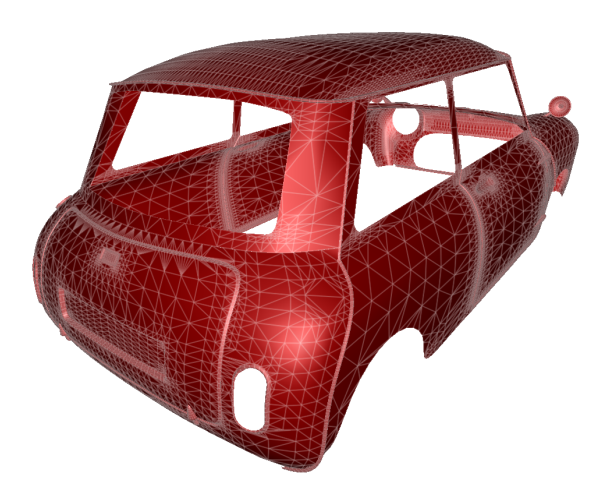
\includegraphics[width=0.35\linewidth]{obrazky-figures/wireframe1.png}
    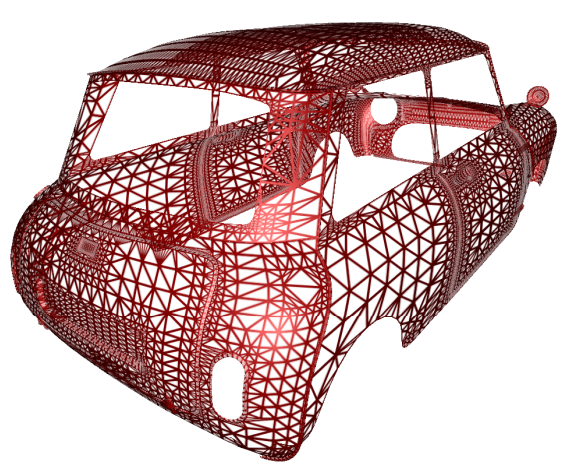
\includegraphics[width=0.35\linewidth]{obrazky-figures/wireframe2.png}
    \caption{Grafický objekt so zvýraznenými primitívmi \cite{wireframeObr}.}
\end{figure*}

\section{Postup vykresľovania objektov na GPU a Shadery}
\label{renderingOnGPU}
Rasterizácia \cite{GraphicsPipeline} je proces mapovania geometrie definovanej vo vektorovom formáte na dvoj-dimenzionálnu mriežku (obrazovku). Samotný postup tohto procesu je vcelku jednoduchý a je ho možné rozdeliť do sekvencie nasledovných krokov:
\begin{enumerate}
    \item Koordinačné vektory vstupných geometrických vrcholov sa vynásobia transformačnou maticou na určenie pozície vrcholu na obrazovke.
    \item Trojuholníky zložené z~týchto vrcholov, ktoré sa nachádzajú na obrazovke, sa zaplnia fragmentami (pixlami) obrazovky.
    \item Výsledné fragmenty sa zoradia podľa pozícii na obrazovke a hĺbky. Ak sa dva fragmenty nachádzajú na rovnakom mieste, tak sa zahodí fragment s~väčšou hĺbkou od~pohľadu kamery.
    \item Každému zvyšnému fragmentu je pridelená korešpondenčná farba.
\end{enumerate}

Softvérová aplikácia \cite{GraphicsPipeline} získava prístup ku grafickému hardvéru a teda k~tomuto procesu pomocou špecializovaných knižníc ako napríklad OpenGL. Pomocou takejto knižnice vieme identifikovať a inicializovať konkrétny grafický hardvér, vytvoriť dátové úložiská s~geometrickými informáciami a pripojiť tieto úložiská ako vstupné hodnoty pre rasterizačný proces.

Grafický hardvér spoločne s~aplikačnými knižnicami vytvárajú vykresľovací reťazec  \cite{GraphicsPipeline} (pipeline). Proces, ktorý je vykonávaný v~tomto reťazci sa volá renderovanie. Pozostáva z~rôznych fáz, z~ktorých každá vykonáva nejakú konkrétnu úlohu. Tieto fázy korešpondujú s~jednotlivými krokmi v~rasterizácii. Väčšina z~týchto krokov sú programovateľné a preto si ich vie užívateľ upraviť podľa seba:
\begin{itemize}
    \item Ovládač vstupu \,--\, Číta dáta z~užívateľských úložísk a skladá ich do primitívov,
    \item Vertex shader \,--\, Programovateľný krok na operácie nad vrcholmi,
    \item Surface shader \,--\, Programovateľný krok, v~ktorom sa pripravujú dáta pre tesalátor,
    \item Tesalátor \,--\, Počíta detailné geometrické povrchy,
    \item Domain shader \,--\, Programovateľný krok, v~ktorom sa počíta pozícia vrcholov na základe výsledkov teselátora,
    \item Geometry shader \,--\, Programovateľný krok, ktorý vie generovať dodatočné vrcholy,
    \item Rasterizátor \,--\, Prevádza vektorové informácie do rasterizovaného obrazu,
    \item Fragment shader \,--\, Programovateľný krok pre operácie nad fragmentami obrazu,
    \item Spájanie výstupu \,--\, Vygenerovanie finálnych farieb pre pixely na obrazovke.
\end{itemize}
Nie všetky kroky v~tomto procese sú povinné pri vytváraní grafickej aplikácie. Zvyšná časť sekcie sa venuje shaderom ktoré boli využité vo finálnej aplikácii.

\subsection*{Vertex shader}
Vertex shader \cite{RTRend} je prvý krok pri spracovaní trojuholníkov skladajúcich sa z~vrcholov objektu. Tieto vrcholy sa skladajú z~pozície v~objekte, prípadne jeho normálovej hodnoty, farby alebo pozícii na textúre. Avšak dáta o~konkrétnych trojuholníkoch, nemá shader k~dispozícii. Zaujímajú ho len prichádzajúce vrcholy.

Umožňuje upravovať, vytvárať alebo aj ignorovať hodnoty spojené s~vrcholom ako jeho pozíciu, farbu alebo normálovú hodnotu. Vždy však musí preniesť pozíciu vrcholu v~objekte do jednotného dvojrozmerného priestoru a túto hodnotu poslať ďalej do reťazca na~rasterizáciu. 

Na každom vrchole sa v~grafike pracuje samostatne a paralelne, preto vypočítané hodnoty na jednom vrchole neovplyvňujú ostatné. Každá vypočítaná hodnota sa však interpoluje vrámci celého trojuholníka a nemusíme teda napríklad počítať farbu každého fragmentu v~trojuholníku.

\subsection*{Fragment shader}
Vypočítané interpolované hodnoty z~vertex shaderu sa stávajú vstupné hodnoty pre fragment shader \cite{RTRend}. Kedže sa nachádza fragment shader za rasterizátorom, každý fragment pozná svoju pozíciu na obrazovke. Úlohou fragment shadera býva zafarbiť daný pixel konkrétnou farbou.

Limitácia fragment shaderu je, že dokáže ovplyvňovať len fragment na jednej pozícii. Nevie čítať ani upravovať vstupy svojich susedných fragmentov.

\section{Kamerová projekcia}
\label{KameraTeoria}
Kamerová projekcia \cite{transf&proj} slúži k~projekcii objektov v~scéne do dvojrozmernej roviny, podobne ako fotoaparát alebo kamera v~reálnom svete. Medzi najviac využívané typy projekcií v~počítačovej grafike sa radí ortogonálna a perspektívna projekcia.

\subsection*{Ortogonálna projekcia}

Ak sa použije ortogonálna projekcia \cite{RTRend}, tak si všetky objekty uchovávajú svoju veľkosť nezávisle od ich vzdialenosti od kamery. Matica \ref{MaticaOrt} ukazuje jednoduchú ortogonálnu maticu, ktorá necháva x- a y-hodnoty nezmenené zatiaľ čo nastavuje hodnotu z~na nulu. Premieta všetky body objektu na rovinu $z = 0$.
\begin{equation} \label{MaticaOrt}
    O = 
    \begin{pmatrix}
    1 & 0 & 0 & 0\\
    0 & 1 & 0 & 0\\
    0 & 0 & 0 & 0\\
    0 & 0 & 0 & 1\\
    \end{pmatrix}
\end{equation}

Obrázok \ref{ortogonal} ukazuje objekt vykreslený ortogonálnou projekciou z~každej roviny obkolesenej kocky.

\begin{figure*}[t]
    \centering
    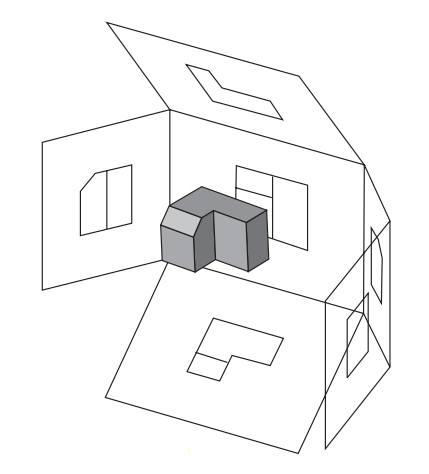
\includegraphics[width=0.4\linewidth]{obrazky-figures/ortogonal.png}
    \caption{Objekt vykresľovaný ortogonálnou projekciou \cite{transf&proj}}
    \label{ortogonal}
\end{figure*}

Projekcia týchto objektov \cite{RTRend} je rozdielna od projekcie v~reálnom svete, kedže v~skutočnosti sa nám objekty ktoré sú vzdialenejšie od kamery zdajú byť menšie. Pre projekciu podobnú skutočnému svetu je potrebné použiť perspektívnu projekciu.

 \subsection*{Perspektívna projekcia}

Komplexnejšia transformácia ako ortogonálna projekcia je perspektívna projekcia \cite{RTRend}, ktorá sa pravidelne používa pri väčšine aplikácií počítačovej grafiky. Paralelné čiary v~tejto projekcii nemusia zostať paralelné a môžu konvergovať do jedného bodu. V~obrázku \ref{perspective} je~vidno v~časti (a) plochú rovinu a v~časti (b) tú istú rovinu ale konvergujú k~jednému bodu, čo~vytvára ilúziu hĺbky. Následne je v~časti (c) udržaný efekt hĺbky aj bez konvergentného bodu a v~časti (d) je tento efekt použitý na vytvorenie kvázi miestnosti.

\begin{figure*}[b!]
    \centering
    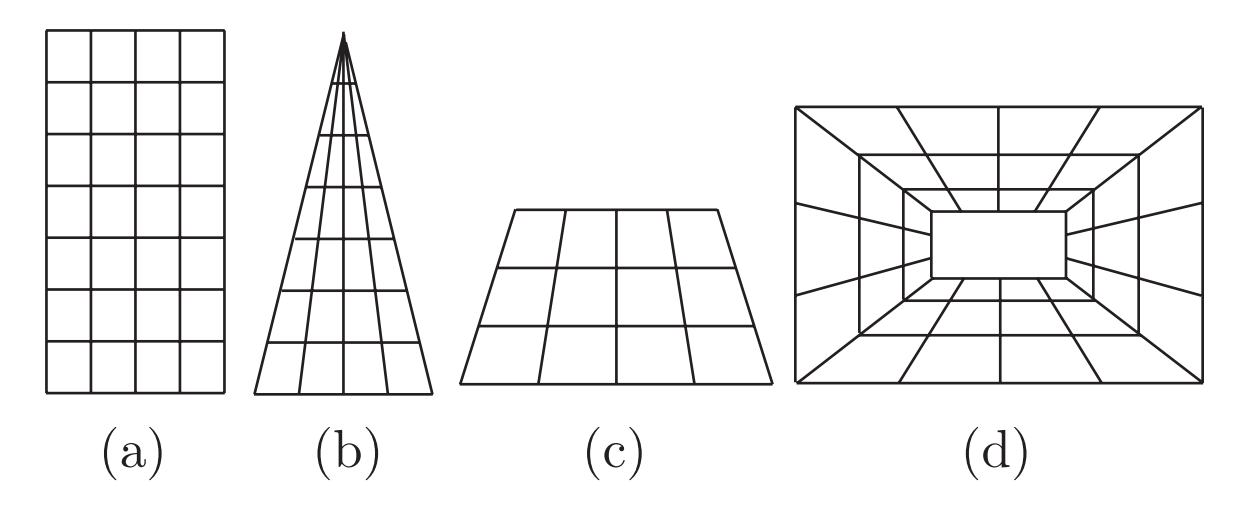
\includegraphics[width=0.7\linewidth]{obrazky-figures/perspective.png}
    \caption{Ukážka perspektívnej projekcie \cite{transf&proj}}
    \label{perspective}
\end{figure*}
\newpage

\noindent Perspektívna matica \cite{RTRend} na zobrazenie scény je zobrazená v~matici \ref{MaticaPer}. Skratky hodnôt znamenajú:

\begin{itemize}
    \item l  \,--\, Ľavá hodnota roviny obrazovky,
    \item r  \,--\, Pravá hodnota roviny obrazovky,
    \item b  \,--\, Spodná hodnota roviny obrazovky,
    \item t  \,--\, Vrchná hodnota roviny obrazovky,
    \item n  \,--\, Hodnota hĺbky najbližšie sa zobrazujúcich objektov,
    \item f  \,--\, Hodnota hĺbky najďalej sa zobrazujúcich objektov.
\end{itemize}

\begin{equation} \label{MaticaPer}
    P = 
    \begin{pmatrix}
    \frac{2n}{r - l} & 0 & -\frac{r + l}{r - l} & 0\\
    0 & \frac{2n}{t - b} & -\frac{t + b}{t - b} & 0\\
    0 & 0 & \frac{f + n}{f - n} & -\frac{2fn}{f - n}\\
    0 & 0 & 1 & 0\\
    \end{pmatrix}
\end{equation}

Po vynásobení maticou \ref{MaticaPer} \cite{RTRend} vznikne bod $q = (q_x, q_y, q_z, q_w)$, takže na zistenie reálnej hodnoty bodu je treba ešte spočítať nový bod $p = (q_x/q_w, q_y/q_w, q_z/q_w, 1)$. Tieto hodnoty už sú správne.

\section{Mračno bodov}
\label{MracnoBodov}
Mračno bodov je sada bodov \cite{pointClouds}, kde každý bod reprezentuje nejaké miesto v~trojdimenzionálnom priestore. Môže sa skladať z~miliónov jedinečných políčok, kde každé obsahuje minimálne polohu bodu. Na samotné vykreslenie bodov to stačí, ale body často obsahujú informácie naviac ako napríklad farba bodu alebo normálový vektor. Ak je týchto bodov v~mračne dostatok vieme ich využiť na vykresľovanie objektov v~scéne. Takto vykreslený objekt je viditeľný na obrázku \ref{PC}. Je to veľmi účinná metóda ako uchovať objekt z~reálneho sveta v~digitálnej podobe.

Na zaznamenanie sa môže použiť laserový skener, fotogrametria alebo sa dá vygenerovať softvérom nad grafickou scénou. Laserový skener býva kvalitnejšia metóda ako fotogrametria pretože laser dokáže presne identifikovať pozíciu bodu v~priestore a vie to spraviť s~extrémnou presnosťou. 
\begin{figure*}[b!]
    \centering
    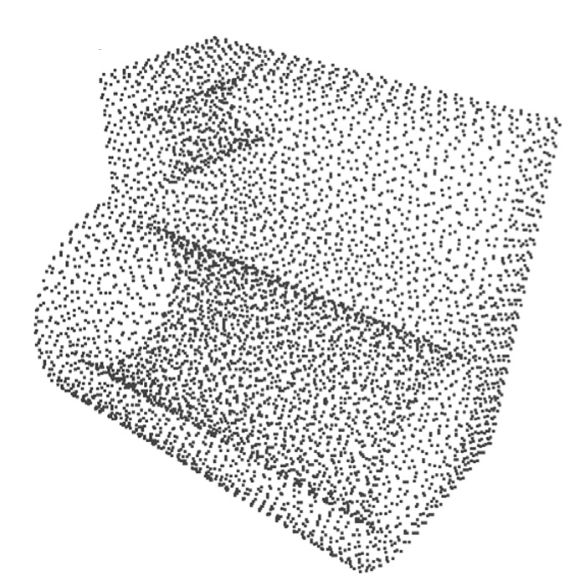
\includegraphics[width=0.275\linewidth]{obrazky-figures/PC.png}
    \caption{Objekt zobrazený ako mračno bodov \cite{PCImg}}
    \label{PC}
\end{figure*}

\section{Tepelná mapa a akceleračné štruktúry}
\label{HMlabel}
Tepelná mapa je dvojrozmerná grafická reprezentácia dát \cite{Heatmaps_intro}, kde sú hodnoty premenných zobrazované ako farby. Príklad tepelnej mapy sa nachádza v~obrázku \ref{HeatMap}. Tepelné mapy sú dôležité kvôli dvom dôvodom. Prvým dôvodom je to, že intuitívne farby použité vo~farebnej škále inšpirované teplotou, znižujú čas potrebný na pochopenie mapy. Je známe, že~žltá je~teplejšia ako zelená, oranžová je teplejšia ako žltá a červená je horúca. Následne~je jednoduché pochopiť že \uv{teplota} farby je priamo úmerná hodnote v~bode. Druhý dôvod je, že tepelné mapy zobrazujú hodnotu priamo nad meraným priestorom. 

Kvôli tomuto je tepelná mapa veľmi účinná pri vizualizácii meraných hodnôt pri porovnaní s~klasickým zobrazením numerických hodnôt. Tepelné mapy nám umožňujú si rýchlo všimnúť prípadné vzory alebo sklony v~dátach.
\begin{figure*}[t]
    \centering
    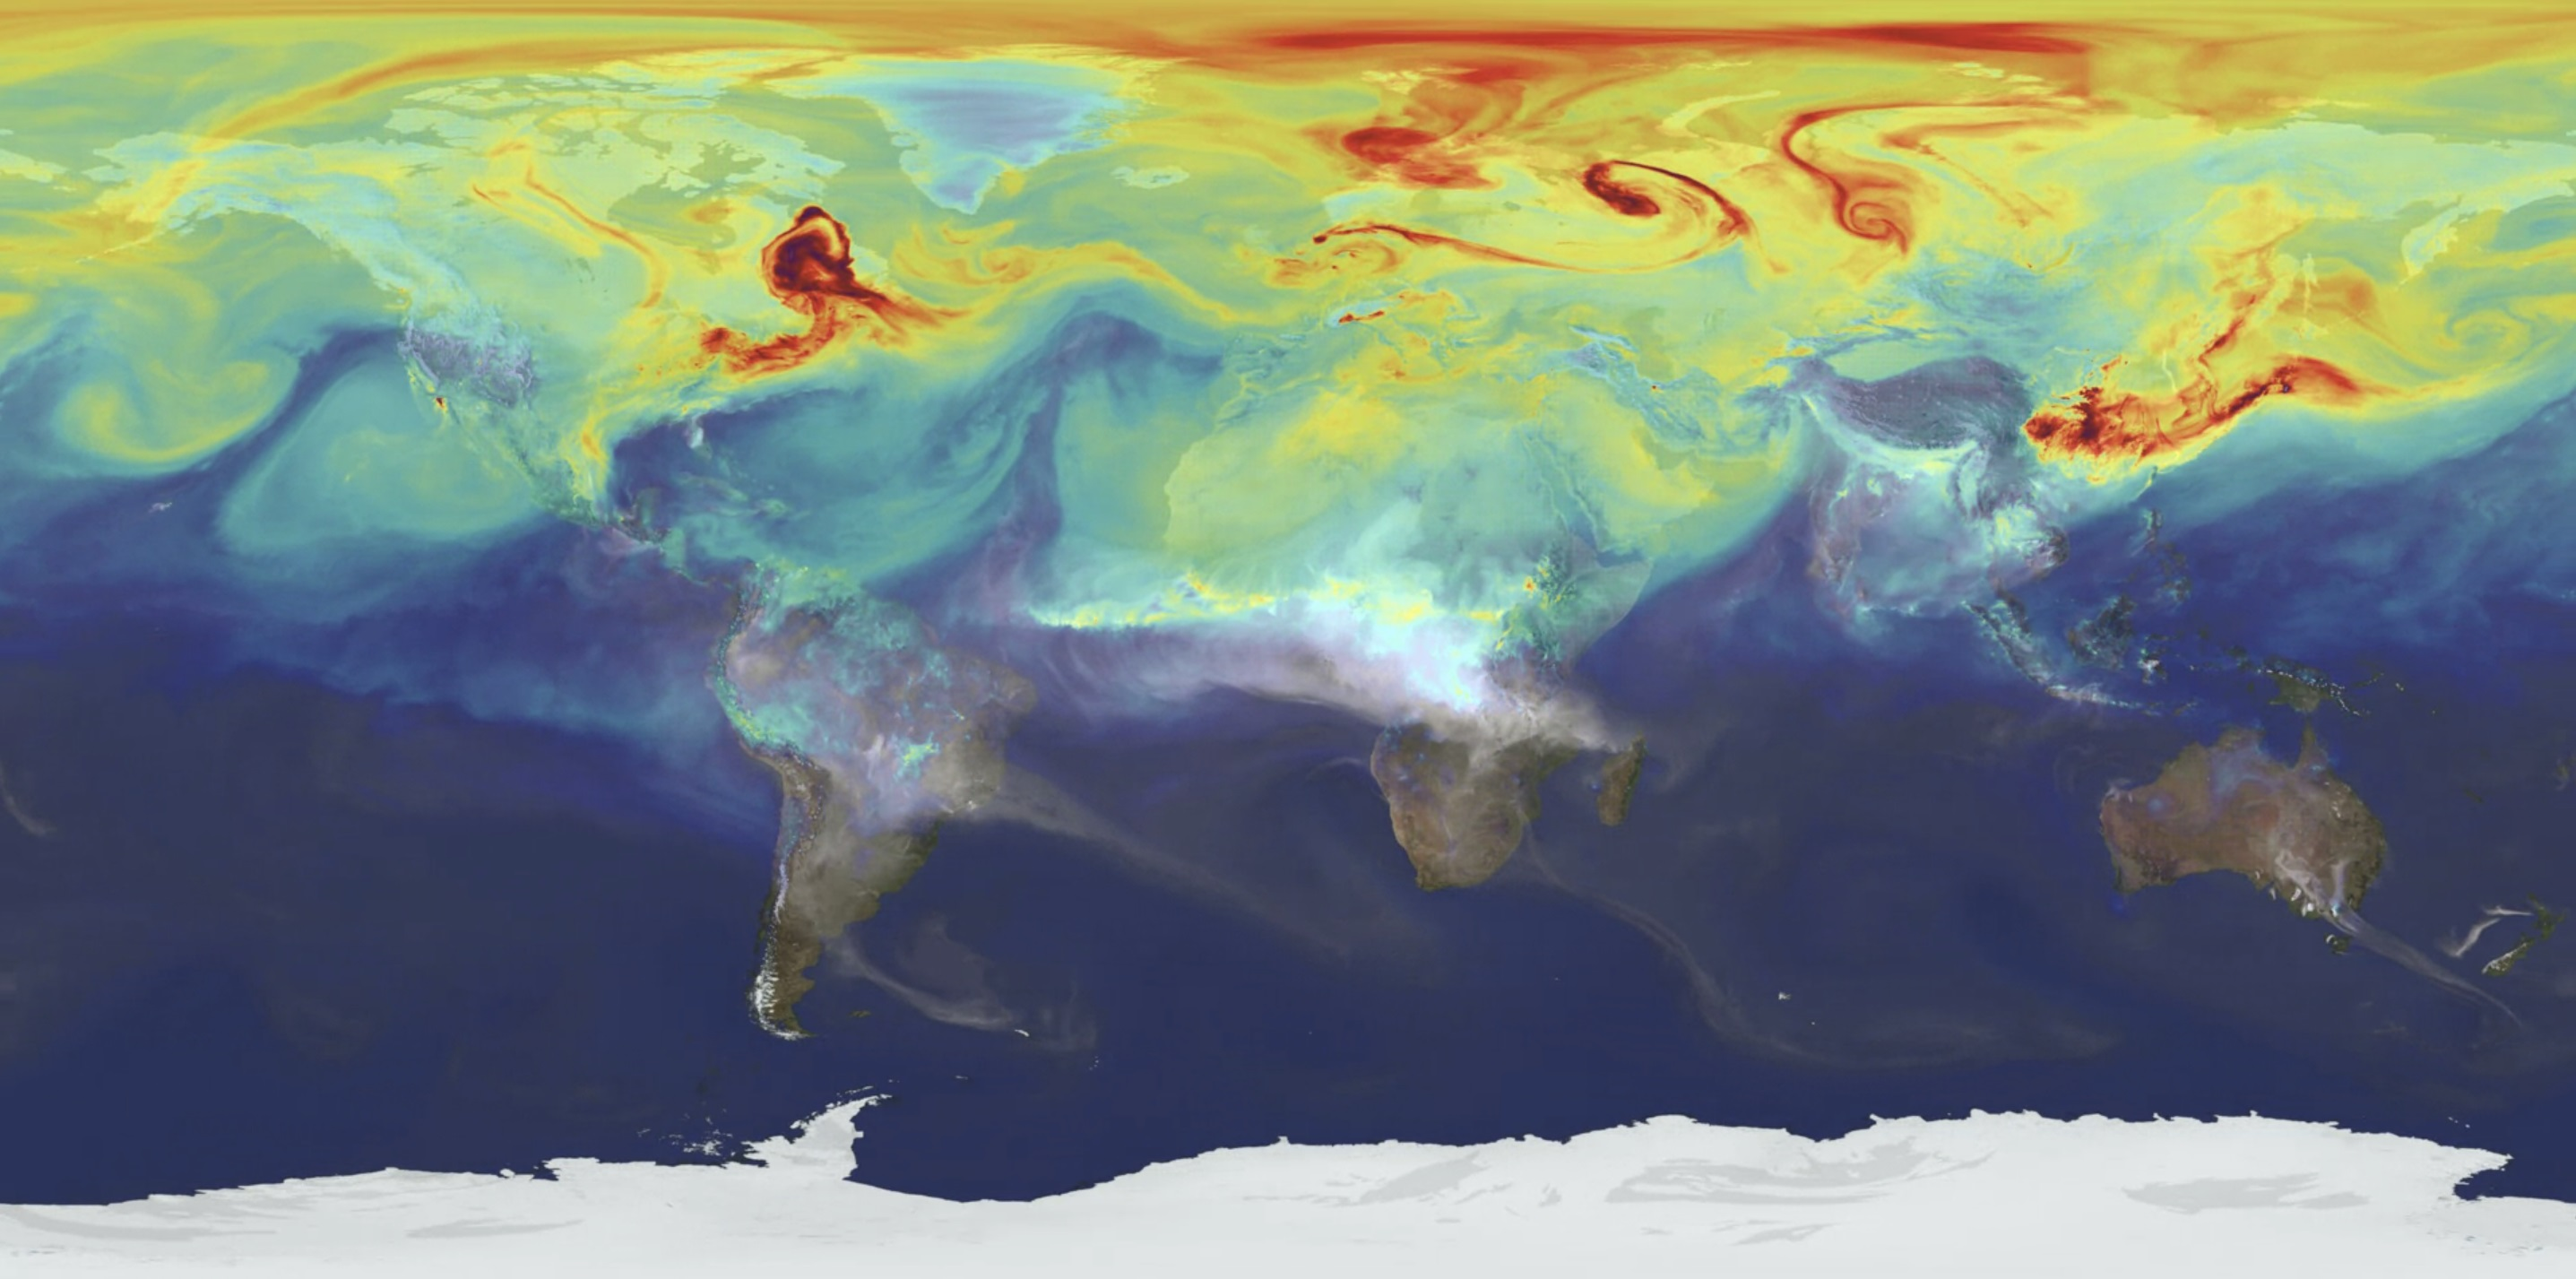
\includegraphics[width=0.75\linewidth]{obrazky-figures/World_heat_map.jpg}
    \caption{Hodnoty teploty namerané vo svete z~dňa 5. apríla 2019 \cite{heatmapwiki}}
    \label{HeatMap}
\end{figure*}

Pri práci s~obrovským obsahom dát, hlavne pri vykresľovaní v~reálnom čase, je potrebné zaručiť rýchly prístup k~dátam. Na tieto účely existujú akceleračné štruktúry.

\subsection*{k-D stromy}
k-D strom je binárny vyhľadávací strom\cite{KDTrees}, kde dáta v~každom uzle majú k-dimenzionálnu pozíciu v~priestore. Nelistový uzol v~k-D strome rozdeľuje priestor do dvoch častí, nazývané polo-priestory. Body naľavo od tohto priestoru sú reprezentované ľavým podstromom a~body napravo zase pravým podstromom.

Pre generalizáciu sa dá očíslovať rovina pre každú jednu dimenziu stromu. Roviny sú teda očíslované $0, 1, 2, ... (k-1)$. Bod v~hĺbke $d$ je orientovaný podľa roviny $A$ ktorá je vypočítaná $A = d \mod k$. Ak je koreňový uzol orientovaný podľa roviny $A$, tak ľavý podstrom obsahuje všetky body, ktorých hodnota polohy na rovine $A$ je menšia ako v~koreňovom uzli. Podobne v~pravom podstrome sú všetky body, ktorých hodnota je väčšia.

Pre ďalšiu akceleráciu sa dajú jednotlivé body ukladať do tried podľa klasifikačných algoritmov. Následne pri kalkuláciách stačí rátať len s~bodmi v~konkrétnych triedach.

\subsection*{kNN algoritmus}
kNN (k-Nearest Neighbor) je klasifikačný algoritmus \cite{KNNSearch} ktorý pracuje na princípe žiadnych predpokladov. Tento princíp znamená že algoritmus nerobí žiadne predpoklady ohľadom parametrov. Bod je klasifikovaný podľa najpočetnejšej triedy jeho susedov. Ak je $k = 1$ tak bod len zdedí triedu najbližšieho suseda. Ak je $k > 1$ tak sa zdedí trieda s~najväčším zastúpením medzi susedmi. Trieda $y$ sa dá predpovedať pomocou rovnice \ref{KNN}:

\begin{equation} \label{KNN}
    y = \arg \max_{(c)}\Big{[} \sum^{K}_{i=0} I_c(n_i) \Big{]},
\end{equation}

\noindent kde:
$$I_c(n) = 1, \text{ak } n \in \text{v triede c.}$$

\subsection*{kNN s~váhou}
kNN s~váhou je variant kNN algoritmu. Najjednoduchší spôsob je spočítať dominantnú triedu v~KNN. Problém môže nastať ak vzdialenosti najbližších susedov sú príliš rozdielne a~napríklad susedia ktorý sú vzdialenejší prehlasujú bližšieho suseda. Kvôli tomuto problému sa vymyslel vážený KNN algoritmus.

Ak $k > 1$ Každý sused má priradenú váhu, ktorá je využitá pri priraďovaní triedy. Táto váha $W_n$ môže značiť napríklad inverznú vzdialenosť suseda od bodu. Bod sa~priradí do~takej triedy, ktorej suma po zrátaní všetkých susedov bola najväčšia. Táto trieda $y$ sa dá predpovedať pomocou funkcie \ref{WKNN}.
\begin{equation} \label{WKNN}
    y = \arg \max_{(c)}\Big{[} \sum^{K}_{i=0} I_c(n_i) W_{n_i} \Big{]}
\end{equation}
\subsection*{kNN s~váhou a predpokladom triedy}
kNN s~váhou a predpokladom triedy \cite{KNNSearch} používa pravdepodobnosť že bod bude patriť do niektorej z~tried. Táto pravdepodobnosť sa používa pri klasifikovaní bodu. Ak je $k > 1$ pravdepodobnosť sa počíta na každom susedskom bode.

Ak $c_1$ je majoritná trieda a $c_2$ je minoritná, tak sa pravdepodobnosť týchto tried dá vypočítať pomocou rovníc \ref{CCW1} a \ref{CCW2}:

\begin{equation} \label{CCW1}
    L_1 = \sum^n_{i=1} p(x_i \mid y_i = c_1),
\end{equation}

\begin{equation} \label{CCW2}
    L_2 = \sum^n_{i=1} p(x_i \mid y_i = c_2),
\end{equation}

\noindent a trieda $y$ sa dá predpovedať pomocou rovnice \ref{CCW3}:

\begin{equation} \label{CCW3}
    y = \arg \max_{(c)}\Big{[} p(x_i \mid y_i) \sum^{K}_{i=0} I_c(n_i) \Big{]}.
\end{equation}

\section{Hemisférické harmonické funkcie}
\label{HSHlabel}
Sférické harmonické funkcie (SH) reprezentujú funkcie definované na guli \cite{HSH}. V~grafických aplikáciách sa používajú hlavne na reprezentáciu funkcií na odraz svetla od povrchu objektu (BRDF) alebo na environmentálne mapy. Pri použití oboch sa hodnota svetelného integrálu dá zapísať ako skalárny súčin vektorov. Naviac sa SH dajú využiť aj pre uloženie predom vypočítaných tieňov a dát vnútorných odrazov. Avšak tieto funkcie ako tieňovanie, vnútorné odrazy alebo BRDF sú definované na pologuli, zatiaľ čo základné SH funkcie sú definované na celej guli. Preto je potrebných viacero koeficientov SH pre presnejšiu reprezentáciu.

Pre vyriešenie tohto problému sa môžu použiť hemisférické harmonické funkcie (HSH). Tieto hemisferické funkcie sú adaptáciou na verziu SH, ktorá sa spolieha na združené Legendreove polynómy. V~HSH sa tieto polynómy posúvajú pre vytvorenie nového základu.

\subsection*{Ortogonálne polynómy}
Množina polynómov $\{p_1(x)\}$ sú ortogonálne \cite{HSH} v~intervale $[a,b]$ ak $p_1(x)$ je polynóm stupňa $l$, pre $n,m \geq 0$:
\begin{equation} \label{OP}
    \int^b_a w(x)p_n(x)p_m(x) \text{dx} = \delta_{nm}c_n,
\end{equation}

\noindent kde $\delta_{nm}$ je 0 alebo 1 ak $n \neq m$ alebo $n = m$ a $w(x)$ je pozitívna funkcia váhy. Ak $c_n = 1$ tak sú polynómy ortonormálne.

\subsection*{Posunuté polynómy}
Posúvanie je lineárna transformácia \cite{HSH} $x$ do $k_1x + k_2$, pričom $k1 \neq 0$. Ak sú polynómy $\{p_1(x)\}$ ortogonálne na intervale $[a,b]$ s~funkciou váhy $w(x)$, tak polynómy $\{p_1(k_1x+k_2\}$ sú ortogonálne na intervale $[\frac{a-k_2}{k_1}, \frac{b-k_2}{k_1}]$ s~funkciou váhy $w(k_1x + k_2)$. Ak $\{p_1(x)\}$ sú ortonormálne tak aj $\{(\pm k_1)^l \sqrt{| k_1 |}p_l(k_1x + k_2)\}$ sú ortonormálne. Polynómy $\{p_l(k_1x+k_2)\}$ sú posunuté verzie $\{p_l(x)\}$.

\subsection*{Asociované Legendreove polynómy}
Asociované Legendreove polynómy (ALP) \cite{HSH}, $\{P_l^m(x)\} \text{pričom } m \in \{0,\dots,l\}$, sú množiny ortogonálnych polynómov na intervale $[-1, +1]$ s~ohľadom na na $l$ s~funkciou váhy $w(x) = 1$:
\begin{equation} \label{ZLP}
    \int^1_{-1} P_l^m(x) P_{l'}^{m}(x) \text{dx} = \frac{2(m + l)!}{(2l + l)(l-m)!}\delta_{ll'}.
\end{equation}

Nahradením argumentu $x$ s~$\cos \theta$, sa získa množina funkcií $\{P_l^m(\cos\theta)\}$ definovaných cez uhlový interval $[0, \pi]$. Hodnoty SH funkcií, ortogonálne cez $[0,\pi] \times [0, 2\pi]$, sú zostavené z~$P^m_l(\cos\theta)$ ako:

\begin{equation} \label{ZLP2}
    Y^m_l(\theta, \phi) = 
    \begin{cases}
        \sqrt{2}K^m_l\cos(m\phi)P^m_l(\cos\theta) & \text{ak } m > 0 \\
        \sqrt{2}K^m_l\sin(-m\phi)P^{|m|}_l(\cos\theta) & \text{ak } m < 0 \\
        K^0_lP^0_l(\cos\theta) & \text{ak } m = 0,
    \end{cases}
\end{equation}
kde $K_l^m$ je normalizačná hodnota:
\begin{equation} \label{ZLP3}
    K_l^m = \sqrt{\frac{(2l+1)(l-| m |)!}{4\pi((l+|m|)!)}}.
\end{equation}
\subsection*{Posunuté ALP}
\label{ShiftedALP}
Použitím lineárnej transformácie $x \text{ do } 2x-1$ sa získajú posunuté ALP \cite{HSH} v~intervale $x \in [0,1]$:
\begin{equation} \label{PZLP}
    \Tilde{P}_l^m(x) = P^m_l(2x-1).
\end{equation}
Dôvod tohto posunu je, že po nahradení argumentu $x \text{ s } \cos\theta$, sa získa funkcia $\{\Tilde{P}^m_l(\cos\theta)\}$ ktorá je definovaná na intervale $\theta \in [0, \frac{\pi}{2}]$, čo je rozsah polárneho uhla hemisféry:
\begin{equation} \label{PZLP2}
    \Tilde{P}_l^m(\cos\theta) = P^m_l(2\cos\theta-1) \text{ pričom } \theta \in [0, \frac{\pi}{2}].
\end{equation}

Posunuté ALP zostávajú ortogonálne, ale zmení sa normalizácia podľa definície v~rovnici \ref{PZLP2}. Funkcia \ref{PZLP3} ukazuje ortogonálny vzťah s~ohľadom na $l$, pričom hodnota funkcie váhy je $1$:

\begin{equation} \label{PZLP3}
    \begin{array}{ccc}
     \int_0^1\Tilde{P}_l^m(x)\Tilde{P}_{l'}^m(x) \text{dx} & = & \int_0^1 P_l^m(2x-1)P_{l'}^m(2x-1)\text{dx} \\
         & = & \frac{(m+l)!}{(2l+1)(l-m)!}\delta_{ll'}.
    \end{array}
\end{equation}

\begin{figure*}[!t]
    \centering
    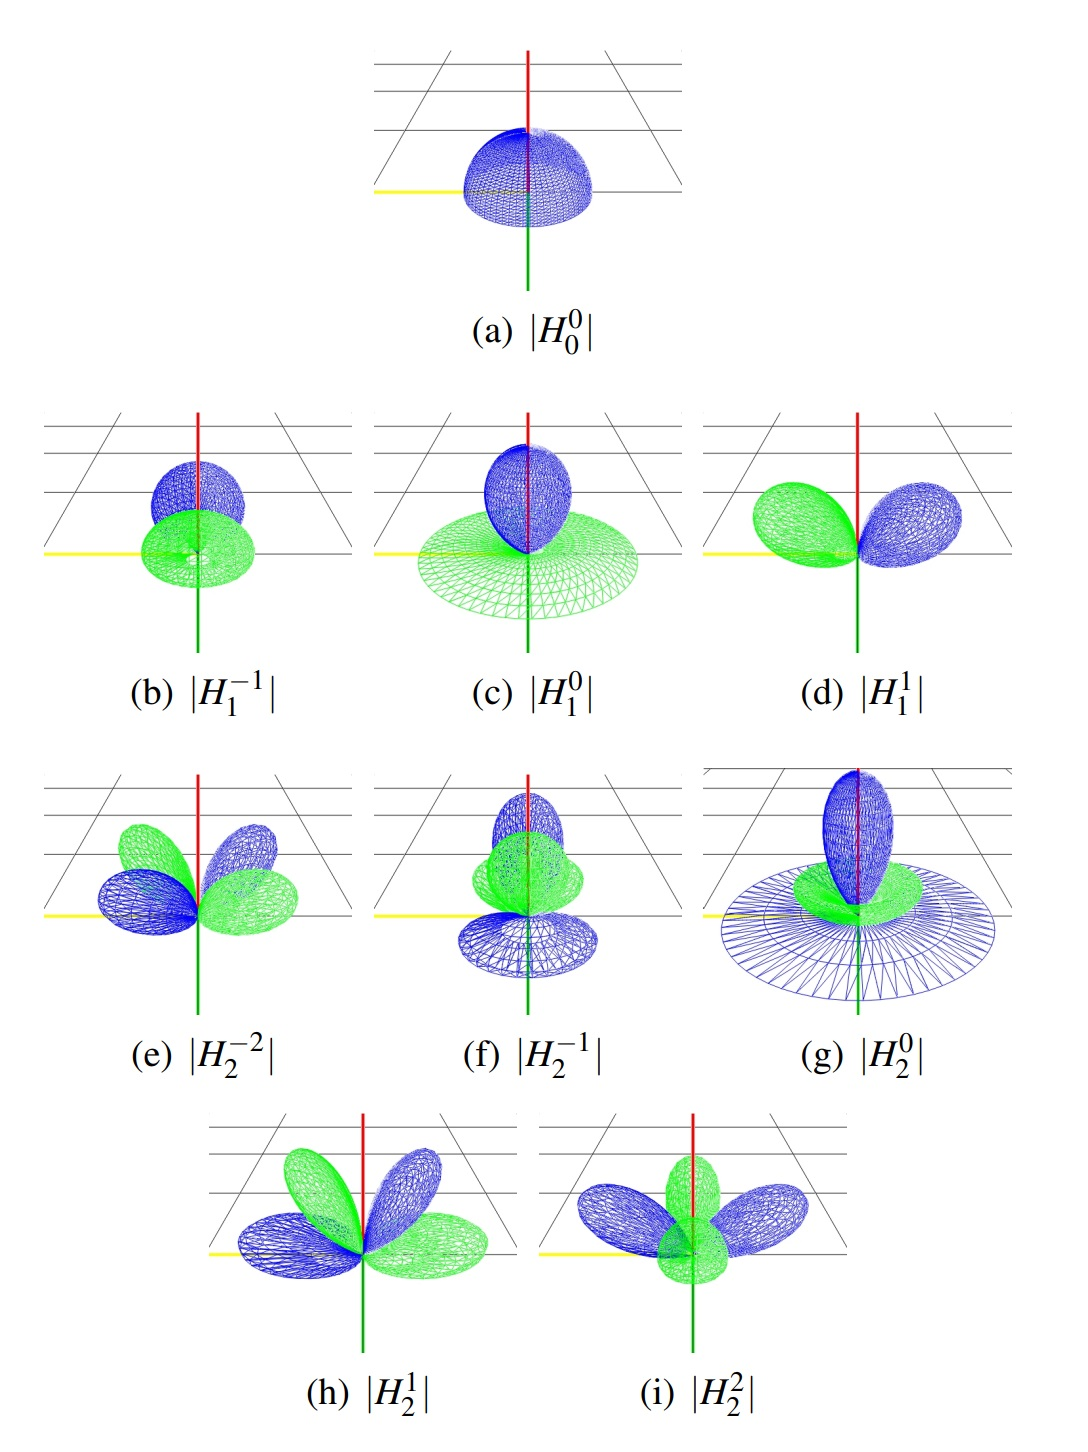
\includegraphics[width=0.35\linewidth]{obrazky-figures/HSH.jpg}
    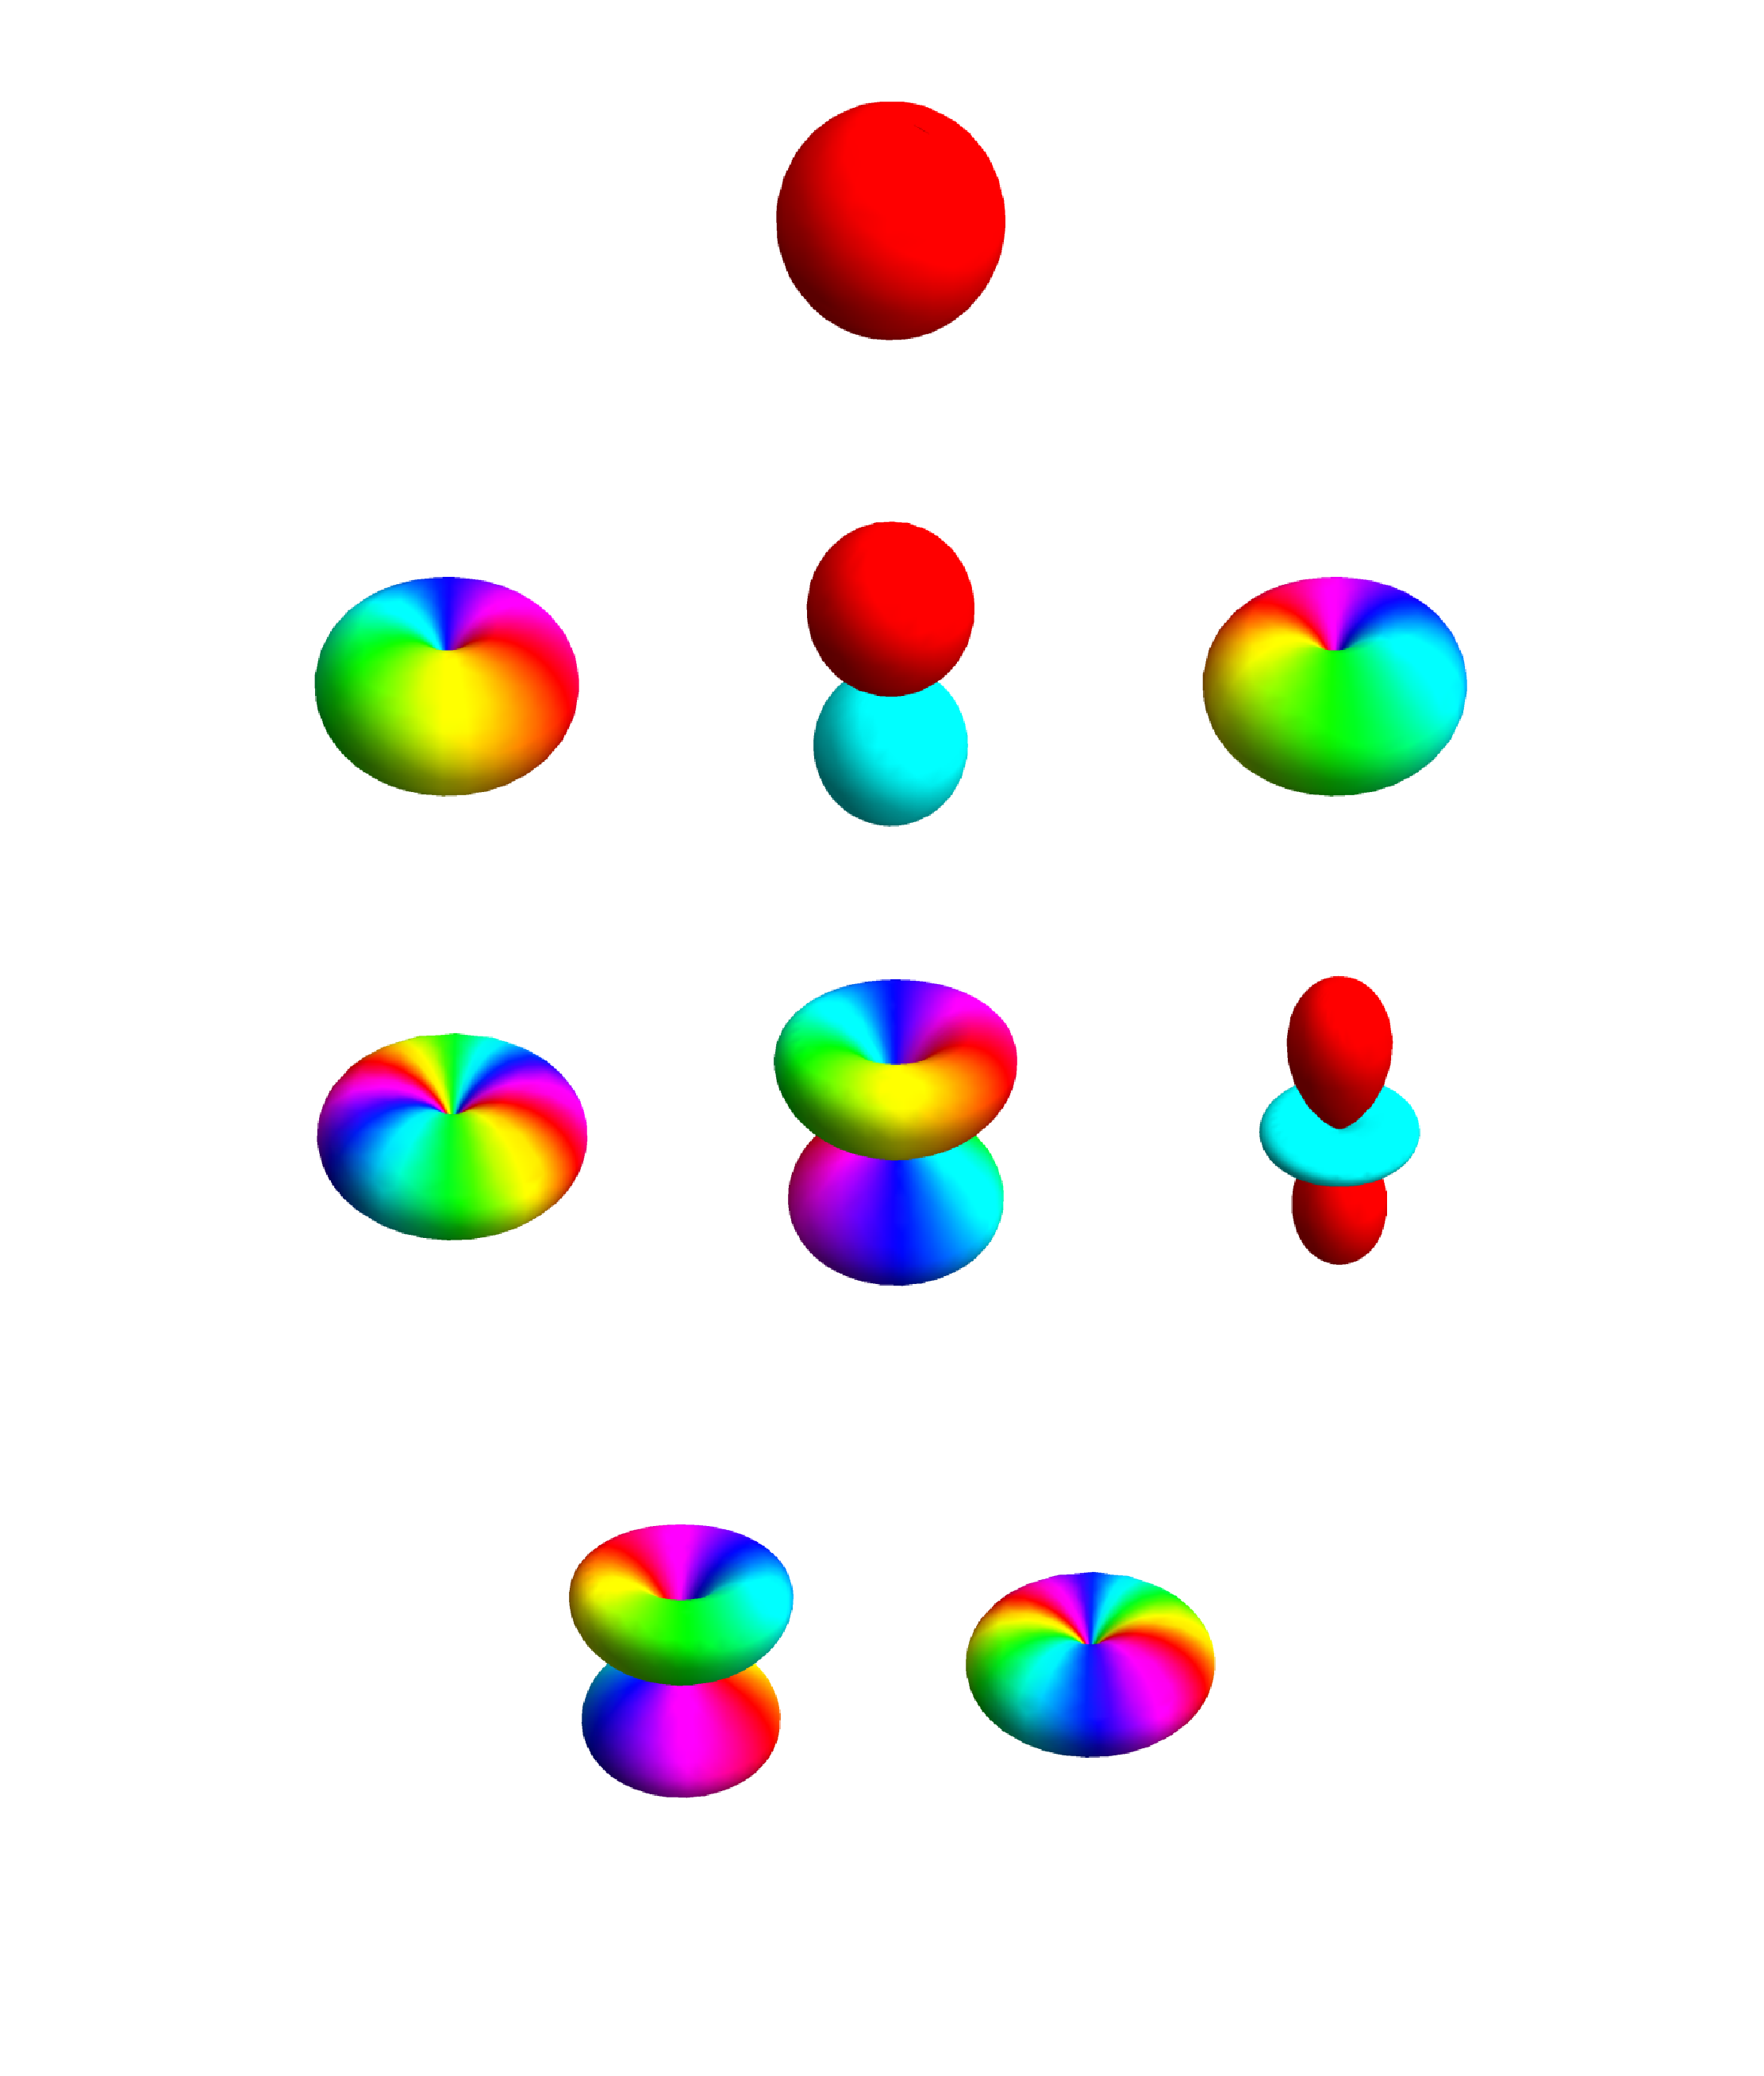
\includegraphics[width=0.35\linewidth]{obrazky-figures/SH2.png}
    \caption{Grafy funkcie $H_l^m \text{ a } Y_l^m$ pre $l \text{ od } 0 \text{ do } 2$\cite{HSH}\cite{SHimg}}
    \label{HSH}
\end{figure*}

\subsection*{Hemisférické funkcie z~posunutých ALP}
Rovnakým spôsobom ako sú SH funkcie zostavené z~ALP, sa zostaví základ aj pre HSH \cite{HSH} $\{H^m_l(\theta, \pi)\}$ z~posunutých ALP:

\begin{equation} \label{HSHA}
        H^m_l(\theta, \phi) = 
    \begin{cases}
        \sqrt{2}\Tilde{K}^m_l\cos(m\phi)\Tilde{P}^m_l(\cos\theta) & \text{ak } m > 0 \\
        \sqrt{2}\Tilde{K}^m_l\sin(-m\phi)\Tilde{P}^{|m|}_l(\cos\theta) & \text{ak } m < 0 \\
        \Tilde{K}^0_l\Tilde{P}^0_l(\cos\theta) & \text{ak } m = 0,
    \end{cases}
\end{equation}

\noindent s~následnou normalizačnou hodnotou:

\begin{equation} \label{HSHA2}
    \Tilde{K}_l^m = \sqrt{\frac{(2l+1)(l-| m |)!}{2\pi((l+|m|)!)}}.
\end{equation}

HSH sú ortogonálne v~rozsahu $[0,\frac{\pi}{2}] \times [0,2\pi)$ s~ohľadom na $l \text{ a aj } m$. Troj-dimenzionálne grafy prvých pár HSH funkcií sú v~obrázku \ref{HSH}.

\section{XML, Mitsuba renderer a Wavefront .obj}
\label{Vstup}
Informácie o~grafickej scéne môžu byť uložené v~rôznych formátoch. Jedným zo spôsobov, ktorý využíva aj Mitsuba renderer, je uchovávať si informácie o~scéne v~súboroch typu XML a informácie o~objektoch v~scéne v~súboroch typu .obj.

\subsection*{XML}
XML (Extensive Markup Language) \cite{XML} je značkovací jazyk umožňujúci anotovanie textových dát pomocou tagov. Základ tohto formátu vychádza zo správne štrukturovaných (well-formed) dokumentov a zameraný je na čitateľnosť a univerzálnu používateľnosť.

Well-formed dokumenty obsahujú značkové elementy, ktoré majú začínajúci a koncový tag, ako v~príklade nižšie:

\begin{verbatim}
    <tag> textové dáta </tag>.
\end{verbatim}

Elementy sa môžu aj vkladať do ostatných elementov a elementové tagy môžu obsahovať aj asociované atribúty. Tieto atribúty poskytujú informácie o~tagu, bez toho aby zasahovali do vložených dát:

\begin{verbatim}
<tag1 atribút1 = "hodnota" atribút2 = "42">
    <tag2> textové dáta </tag2>
</tag1>.
\end{verbatim}

Dokument môže obsahovať pokyny spracovania pre modul XML, ktorý bude čítať dokument a rovnako aj komentáre. Riadia sa však rozdielnou syntaktickou formou ako elementové tagy a môžu sa objaviť na ľubovolnom mieste v~dokumente:

\begin{verbatim}
<?xml-stylesheet type="aplication/xslt + xml" href="#style1"?>
<!- Toto je koment -->.
\end{verbatim}

Dokument musí obsahovať presne jeden element najvyššej úrovne. Poradie elementov je~dôležité, keďže značia tok informácií v~dokumente.

\subsection*{Mitsuba renderer}
\label{TeoriaMitsuba}
Mitsuba renderer \cite{GHMitsuba} je renderovací systém orientovaný na výskum pre obojsmernú simuláciu presunu svetla vyvinutý v~inštitúte EPFL vo Švajčiarsku. Pozostáva z~z~knižníc a~pluginov, ktoré implementujú funkcionalitu pre rôzne materiály a zdroje svetla pre skompletizovanie renderovacích algoritmov. Je postavený na Dr.Jit, špecializovanom just-in-time prekladači zostavenom špeciálne pre Mitsuba renderer. Inštaluje sa pomocou PyPI a funguje ako knižnica pre programovací jazyk Python.

Mitsuba používa na reprezentáciu scén \cite{DocsMitsuba} zjednodušený formát založený na XML. Jednotlivé časti scény sú zapísané ako elementy s~atribútmi obsahujúcimi informácie. Jednoduchá scéna s~jedným objektom bez nasvietenia by vyzerala takto:
\begin{verbatim}
<scene version="3.0.0">
    <shape type="obj">
        <string name="filename" value="mesh.obj"/>
    </shape>
</scene>.
\end{verbatim}

Ostatné časti scény \cite{DocsMitsuba} sa ukladajú podobným spôsobom, ale s~použitím rozdielnych tagov. Priamo v~XML sa dá nastaviť nasvietenie v~scéne, upraviť pozíciu a nastavenia kamery alebo upraviť materiály a transformačné matice objektov. Následne sa dá v~Python kóde ešte upraviť scéna pred samotným renderom. Príklad scény vykreslenej Mitsuba rendererom je na obrázku \ref{MitsubaRender}.

\subsection*{Wavefront .obj}
\label{OBJFormat}
Wavefront .obj \cite{OBJ} je jedným z~najviac používaných formátov pre textové uloženie troj-dimenzionálnych objektov. Geometrické informácie o~objekte ukladá priamo do textového súboru. Niekedy sa k~.obj súboru prikladá .mtl súbor, ktorý označuje materiál z~ktorého sa~objekt skladá.

Formát používa tagy pre špecifikovanie geometrických elementov objektu. Každý tag sa~píše v~samostatnom riadku. Poradie písania elementov je dôležité, pretože pri spájaní plôch sa používa poradie vertexu. Jednotlivé tagy a príklady použitia sú ukázané v~tabuľke~\ref{ObjTable}.

\begin{table}[hb] \label{ObjTable}
\begin{tabular}{lc}
    Komentár: & \# Komentár  \\
    Pozícia vertexu: & v~$x$ $y$ $z$ \\
    Hodnota normálu: & vn $x_n$ $y_n$ $z_n$  \\
    Pozícia na textúre: & vt $x_t$ $y_t$ \\
    Zostavovanie plochy: &  f $v_1/t_1/n_1$ $v_2/t_2/n_2$ $v_3/t_3/n_3$\\
    Zostavovanie plochy len s~vertexom: &  f $v_1$ $v_2$ $v_3$\\
    Zostavovanie plochy s~vertexom a normálom: & f $v_1//n_1$ $v_2//n_2$ $v_3//n_3$\\
    Zostavovanie plochy s~vertexom a textúrov: & f $v_1/t_1$ $v_2/t_2$ $v_3/t_3$
\end{tabular}
\caption{Syntax písania tagov v~.obj formáte \cite{OBJ}.}
\end{table}

\begin{figure*}[hb!] \label{MitsubaRender}
    \centering
    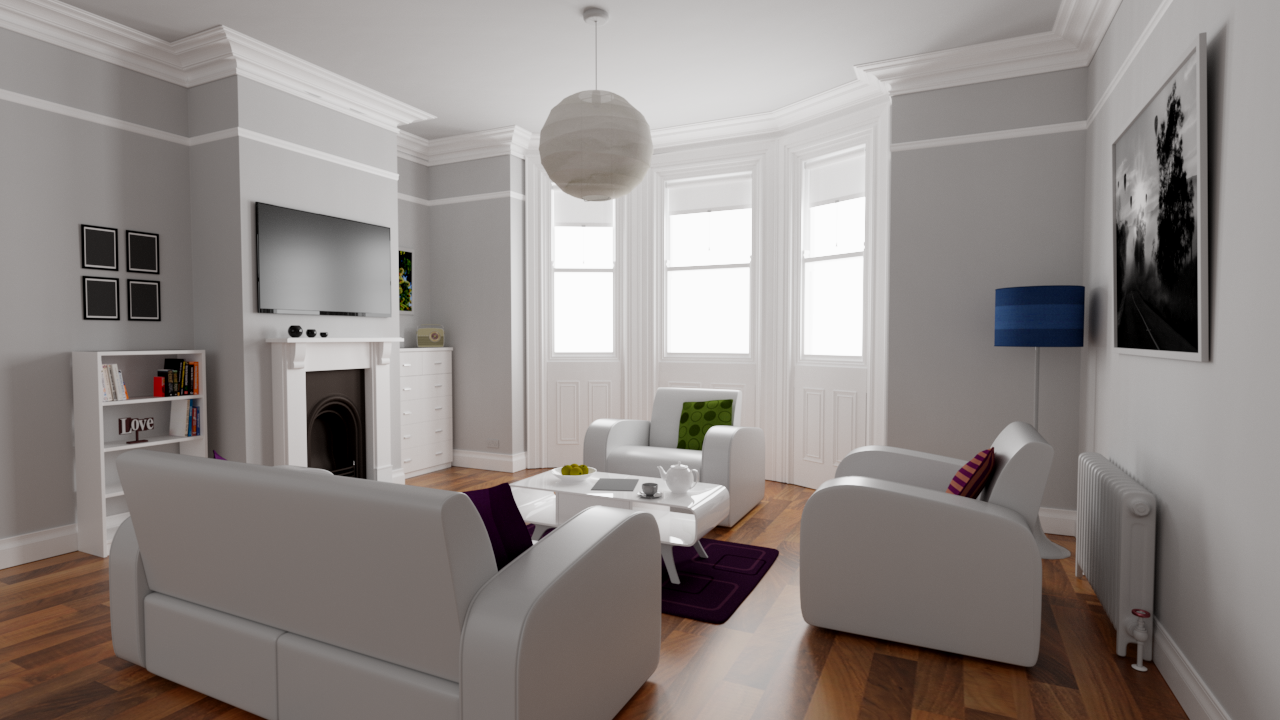
\includegraphics[width=0.90\linewidth]{obrazky-figures/mitsuba_render.png}
    \caption{Scéna vykreslená v~Mitsuba renderer \cite{DocsMitsuba}.}
\end{figure*}

\chapter{Návrh}
\label{Navrh}
Táto kapitola obsahuje návrhy riešení jednotlivých problémov, ktoré bolo treba vyriešiť pri tvorbe aplikácie. Hlavne sa sústredí na parsovanie vstupných dát, návrhom na vykreslenie tepelných máp a hemisférických funkcií a návrhom užívateľského rozhrania. 

V~tejto kapitole sa nachádzajú pojmy, ktoré nemusia byť verejne známe a preto je odporúčané si prečítať kapitolu \ref{Teoria} pre čitateľov, ktorí nie sú oboznámení s~problematikou.
\section{Dáta na vykreslenie}
\label{DataVykreslenie}
\label{DataNavrh}
Pred samotným vykreslením je potrebné si správne prečítať a uložiť vstupné súbory. Okrem súboru s~mračnom bodov, ktorý nemá definovaný presný formát, sú všetky typy súborov bližšie opísané v~sekcii \ref{Vstup}. Diagram návrhu spracovania vstupných dát je na obrázku \ref{diaVstup}. Jednotlivé úseky diagramu sú bližšie vysvetlené v~tejto sekcii.

\begin{figure*}[b!] \label{diaVstup}
    \centering
    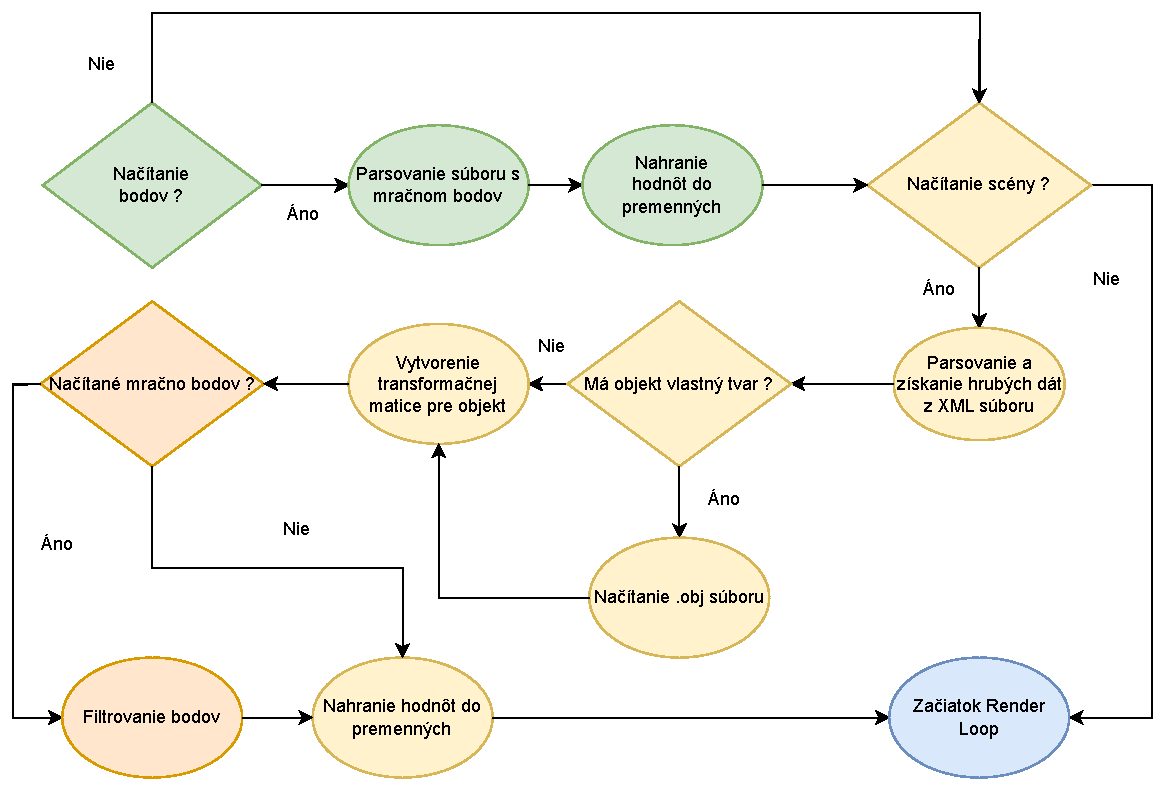
\includegraphics[width=0.80\linewidth]{obrazky-figures/dataLoad.pdf}
    \caption{Návrh načítania vstupných dát}
\end{figure*}
\newpage

\subsection*{Parsovanie súboru s~mračnom bodov}
\label{PointCloudParse}
Súbor s~mračnom bodov \ref{MracnoBodov} má jedinečnú štruktúru a nie je to klasický formát ukladania mračien. Skladá sa z~hodnôt zapísaných v~riadkoch. Každý riadok reprezentuje jeden bod v~mračne. Formát riadku vyzerá takto: $$\Vec{p}, \Vec{s}, \Vec{t}, \Vec{n}, \text{HSH.}$$ 

Hodnoty sú zapísané ako čísla s~desatinou čiarkou. Prvé tri hodnoty zodpovedajú x-,y- a z-koordináciám bodu v~priestore. Nasledujú tangenta, bitangenta a normála bodu. Každá zodpovedá trom hodnotám. 

Koeficienty HSH funkcií \ref{HSHlabel} sa nachádzajú za nimi a môzu mať ľubovolný počet hodnôt. Avšak je potrebné aby každý bod v~mračne mal rovnaký počet koeficientov a aby sa počet koeficientov rovnal $x^2$, pričom $x$ je celé číslo väčšie ako $0$ a označuje rád koeficientov HSH. 

Po úspešnom parsovaní súboru je potrebné uložiť získané hodnoty bodov do pamäte grafickej karty, alebo do premenných pre filtrovanie bodov, ktoré sa vykonáva neskôr v~programe.

\subsection*{Parsovanie XML súboru}
\label{XMLParse}
Vstupný XML súbor je rovnaký ako vstupný súbor v~Mitsuba renderer. Viac o~tomto rendereri je spomenuté v~sekcii \ref{Vstup}. Avšak pre jednoduché zobrazenie scény bez nasvietenia nie je potrebné čítať všetky informácie zo súboru. Zaujímavé sú jedine elementy s~tagom \verb|shape|.

V~týchto elementoch sa nachádzajú informácie o~objektoch v~scéne. Každý \verb|shape| má informáciu o~svojom tvare, prípadne o~transformáciách objektu. Všetky tieto hodnoty je~potrebné uložiť pre následné korektné zobrazenie objektu.

Základný postup pri získavaní hrubých dát z~XML je teda najskôr odfiltrovať len informácie, ktoré sú zaujímavé pre program. Potom uloženie týchto hodnôt do premenných pre ich následné použitie v~programe.

\subsection*{Načítanie .obj súboru a tvorba transformačnej matice}
\label{OBJNavrh}
Element \verb|shape| má tri podporované možnosti tvaru predmetu. Sú to \verb|sphere|, \verb|rectangle| a \verb|obj|. Pri \verb|sphere| a \verb|rectangle| sa načítajú predom určené objekty. V~prípade \verb|obj| je tvar objektu určený .obj súborom. Viac o~.obj súboroch je spomenuté v~sekcii \ref{Vstup}.

Prvý krok pri načítaní .obj súboru je získať k~nemu cestu. Tá je vždy zapísaná v~pod-elementoch typu \verb|obj|, ktoré sú uložené v~premenných. K~tejto ceste je však dôležité pridať aj cestu k~samotnému XML súboru od umiestnenia aplikácie. Pri čítaní .obj súboru je potrebné si uložiť a zoradiť všetky vrcholy a normály. Význam tagov a informácií uložených v~.obj súbore je bližšie popísaný v~sekcii \ref{Vstup}. Pri skladaní primitívov v~tagoch \verb|f| sa~používa práve postupnosť vrcholov a normálov na zostavenie trojuholníkov z~ktorých sa objekt skladá. Toto poradie sa nahradzuje konkrétnymi hodnotami vrcholov a normálov, ktoré sa ukladajú do bufferov (ukladací priestor, vyrovnávacia pamäť). V~bufferoch sú zoradené body a~normály tak, ako budu vykresľované v~primitívoch. Napríklad trojuholník tvoria vždy tri body v~bufferi za sebou. Takto zoradené informácie zo súboru .obj sa nahrávajú do grafickej pamäte.

Transformačná matica pre objekt slúži k~umiestneniu vrcholov objektu do priestoru scény. Vykresľovaniu dát na grafickej karte sa venuje sekcia \ref{renderingOnGPU}. Informácie o~transformáciách sú uložené v~elemente \verb|transform|, ktorý je pod-elementom \verb|shape|. Môžu sa tam rovno nachádzať už zostavené matice, alebo len postupy škálovania, rotácií a posunov objektu. Je potrebné zostaviť transformačné matice pre každý jeden typ transformácie a tie vynásobiť medzi sebou. Keďže násobenie matíc nie je komutatívne, tak je dôležité udržať poradie násobenia. Teda najprv vynásobiť škálovanie s~rotáciou a potom výslednú maticu z~predchádzajúceho výpočtu s~maticou posunu. Finálne transformačné matice sa uložia do~premenných a posielajú sa do pamäte grafiky pri renderovaní objektu s~ktorým súvisia. 

\subsection*{Filtrovanie bodov}
\label{FiltrBodovNavrh}
Filtrovanie bodov slúži na akceleráciu procesu vykreslenia tepelnej mapy. Namiesto toho aby sa pri určovaní zafarbenia v~bode objektu používala vzdialenosť každého bodu v~mračne, tak sa body prefiltrujú aby sa počítalo len s~bodmi, ktoré sa nachádzajú v~blízkosti objektu. Pre každý objekt sa zistí kváder v~ktorý ho ohraničuje. Predtým je však potrebné vrcholy objektu upraviť transformačnou maticou, aby sa nachádzali na správnom mieste z~hľadiska scény.

Pozícia každého bodu z~mračna bodov sa porovná s~kvádrom v~ktorom sa objekt nachádza. Ak sa bod nachádza vnútri kvádru, zaznačí sa. Následne pri renderovaní tepelných máp sa použijú pre každý objekt len body ktoré sú v~jeho blízkosti a tým sa zabráni zbytočnej kalkulácii s~nerelevantnými bodmi.
\section{Operácie na vykreslenie}
\label{OperationsNavrh}
Táto sekcia sa zaoberá návrhmi operácií pri vykresľovaní tepelných máp a hemisférických funkcií. Tieto typy zobrazovania sú bližšie opísané v~sekciách \ref{HMlabel} a \ref{HSHlabel}. 
\subsection*{Tepelné mapy}
\label{HMNavrh}
Diagram návrhu vykreslovania tepelných máp je na obrázku \ref{diaHM}. Vyvinutá aplikácia vie vykresľovať tepelné mapy na vrcholoch objektov a aj na fragmentoch. Pri oboch módoch sa výrazne využíva interpolovanie hodnôt vrcholov v~fragment shaderi. Pri vykresľovaní tepelnej mapy na vrchole sa vypočítaná farba interpoluje medzi fragmentami. Pri vykresľovaní na fragmentoch sa získava pozícia fragmentu v~scéne interpoláciou pozície vrcholov trojuholníkov. Vykresľovanie na fragmentoch je presnejšie ako na vrcholoch, ale zároveň aj~náročnejšie na grafickú kartu.

\begin{figure*}[b!] \label{diaHM}
    \centering
    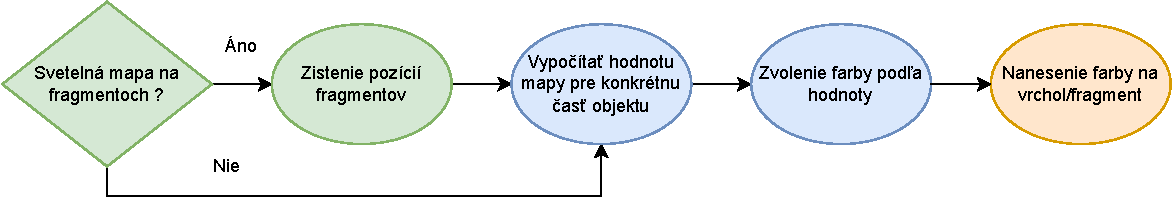
\includegraphics[width=0.80\linewidth]{obrazky-figures/heatmap.pdf}
    \caption{Návrh vykreslenia tepelnej mapy}
\end{figure*}

Pri samotnom počítaní farby je však jedno aký mód sa používa. Pre každý bod z~mračna bodov, ktorý je v~blízkosti objektu, sa vypočíta vzdialenosť od pozície vrcholu/fragmentu. Ak je vzdialenosť dostatočne nízka, začína mať tento bod efekt na zafarbenie. Veľkosť efektu je nepriamo úmerná od vzdialenosti. Efekt každého bodu sa sčítava dokopy. Ak je teda v~blízkosti vrcholu/fragmentu veľa bodov, zvyšuje sa aj hodnota mapy pre konkrétnu časť objektu. Farba sa určí vypočítanou hodnotou, teda ak je hodnota nízka, farba v~bode má odtiene modrej. Ak sa zvyšuje tak začína nadobúdať ostatné farby ako zelenú, žltú alebo červenú. Po zvolení farby sa táto farba nanesie do výstupnej farby vrcholu/fragmentu.

\subsection*{Hemisférické funkcie}
\label{HSHNavrh}

\begin{figure*}[b!] \label{diaHSH}
    \centering
    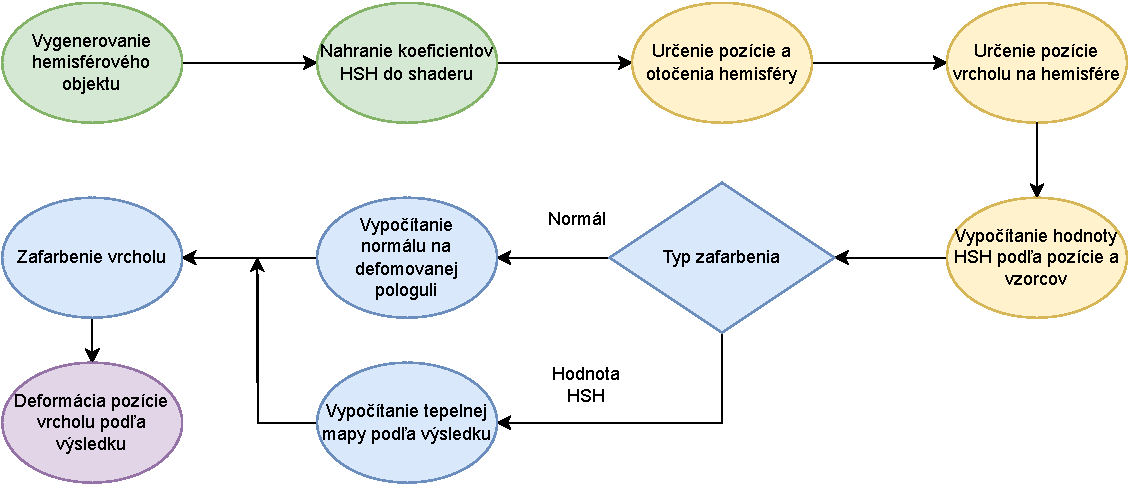
\includegraphics[width=0.70\linewidth]{obrazky-figures/HSHdia.pdf}
    \caption{Návrh vykreslenia hemisférických funkcií}
\end{figure*}

\begin{figure*}[b!] \label{Deform}
    \centering
    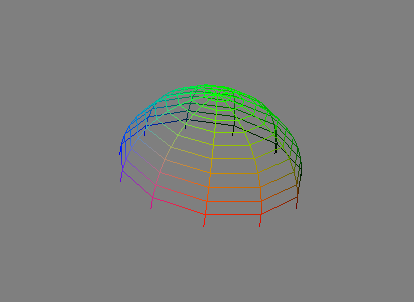
\includegraphics[width=0.35\linewidth]{obrazky-figures/HSHbefore.png}
    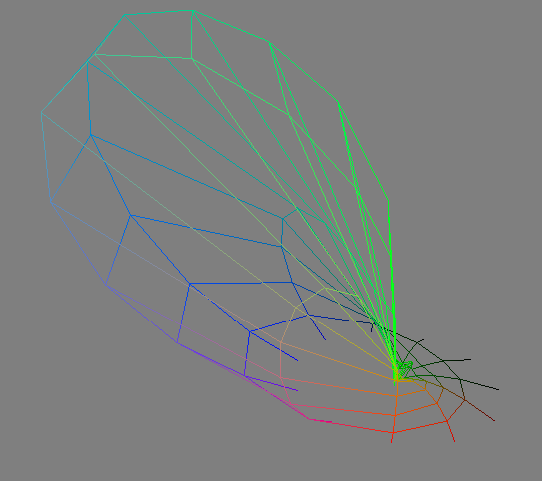
\includegraphics[width=0.3\linewidth]{obrazky-figures/HSHafter.png}
    \caption{Ukážka deformácie pologule}
\end{figure*}

Diagram návrhu vykreslovania hemisférických funkcií je na obrázku \ref{diaHSH}. Konkrétne vzorce na výpočet hodnoty hemisférických funkcií sú v~sekcii \ref{HSHlabel}.

Na začiatku sa vygeneruje hemisférový objekt. Generácia tohto objektu je užitočná pretože sa tým vie kontrolovať kvalita zobrazenia hemisférických funkcií, alebo v~prípade veľkého zaťaženia grafickej karty, znížiť počet vrcholov pre počítanie. Hemisféra má vždy určený počet riadkov a stĺpcov, a skladá sa z~buniek v~tvare štvorcu ktoré vzniknú medzi riadkami a stĺpcami. Ešte pred počítaním je však dôležité nahrať koeficienty HSH do pamäte grafickej karty, aby mohli byť použité vo výpočtoch.

Aby sa hemisféra zobrazovala na správnom mieste a aby bola otočená správnym smerom, je potrebné vypočítať transformačnú maticu na ktorú sa použijú hodnoty pozície, normálu, tangenty a bitangenty bodu. Ďalej je potrebné vypočítať pozíciu samotného vrcholu na~hemisfére. Využíva sa k~tomu vedomosť o~počte riadkov a stĺpcov na hemisfére a~to, že vrcholy boli zoradené od spodu na vrch pri generovaní. Keď je známa pozícia vrcholu na~hemisfére vrámci buniek, je možné zistiť hodnoty y- a z-uhlov, ktoré určujú presnú polohu vrcholu. Tieto hodnoty uhlov spoločne s~Legendreovými polynómami a koeficientami HSH sa využijú na výpočet hodnoty funkcie na vrchole.

Podľa zvoleného typu farbenia týchto funkcií je potrebné vypočítať normály deformovanej pologule alebo využiť výsledok funkcie na vytvorenie jednoduchej tepelnej mapy. Normála sa počíta podľa transformačnej matice a pozícii vrcholu na hemisfére. Tepelná mapa sa počíta ako gradient medzi zelenou a červenou farbou. Pozícia na gradiente sa~určí hodnotou HSH na vrchole. Vypočítaná farba sa~priradí k~vrcholu. Pozícia vrcholu sa nakoniec posunie o~hodnotu výsledku HSH smerom určeným pozíciou vrcholu na hemisfére a~tým sa deformuje pologuľa viď. obrázok \ref{Deform}.

\section{Užívateľské rozhranie}
\label{UINavrh}
Užívateľské rozhranie slúži na interakciu užívateľa s~aplikáciou. V~prípade tejto aplikácie ho reprezentuje okno s~nastaveniami. Tieto nastavenia sa delia do troch častí, kde každá časť sa sústredí na inú oblasť aplikácie. Táto sekcia se venuje priblíženiu funkcií aplikačných nastavení a vysvetleniu navigácie medzi nimi.

\subsection*{Načítanie vstupných súborov a základné nastavenia zobrazovania scény}
V~prvej časti sa nachádzajú nastavenia, ktoré sa zobrazia pri zapnutí aplikácie. Sú zobrazené na obrázku \ref{BSettings}. Políčka \verb|Scene xml file| a \verb|Point Cloud file| obsahujú cesty k~vstupný súborom. Tieto cesty sa dajú zapísať ručne a uložiť tlačítkami \verb|Save scene| a~\verb|Save Point Cloud|. Alternatívne sa môžu použiť tlačítka \verb|Select XML| a \verb|Select Cloud| na~výber súborov pomocou vyskakovacieho okna so súborovým systémom. Pri použití týchto tlačítok sa automaticky vyfiltrujú len typy súborov, ktoré sú podporované aplikáciou.

Nasleduje políčko na úpravu hodnoty, o~ktorú sa zväčši kváder, ktorý pri filtrovaní bodov obkolesuje objekty. Pri renderovaní tepelnej mapy je niekedy užitočné počítať aj s~bodmi, ktoré neležia priamo na objekte. Ak však scéna zaberá väčší priestor je potrebné zväčšiť kváder o~potrebnú hodnotu. Rovnako ak sa scéna odohráva na menšom priestore alebo je renderovanie tepelnej mapy náročné na grafickú kartu, je možné týmto znížiť záťaž alebo spresniť vykresľovanie. Ďalšie tlačítka slúžia na načítanie hodnôt zo vstupných súborov, prípadne na ich uvoľnenie ak už nie sú potrebné.

\verb|Movement Speed| upravuje rýchlosť pohybu kamery v~scéne. \verb|Scene scale| zas škálovanie všetkých objektov v~scéne. Políčko \verb|Vsync| je účinné pri jednoduchých scénach, kedy nieje potrebné grafickú kartu využívať naplno a tak ušetriť grafické zdroje. Pri zaškrtnutí \verb|Wireframe| sa budú vykresľovať len čiary medzi vrcholmi trojuholníkov.
\begin{figure*}[b!] \label{BSettings}
    \centering
    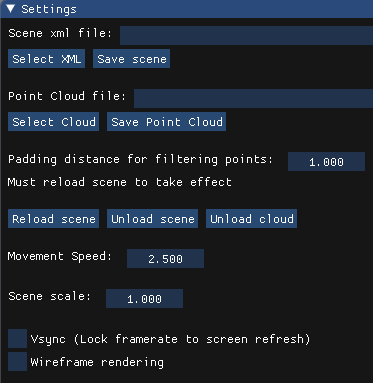
\includegraphics[width=0.40\linewidth]{obrazky-figures/UI_Start.png}
    \caption{Základné nastavenia aplikácie}
\end{figure*}

\subsection*{Nastavenia nad objektami v~scéne}

\begin{figure*}[t!] \label{ObjSettings}
    \centering
    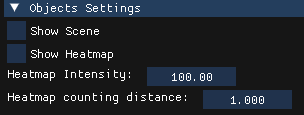
\includegraphics[width=0.45\linewidth]{obrazky-figures/UI_scene.png}
    \caption{Nastavenia objektov v~scéne}
\end{figure*}
V~druhej časti sa nachádzajú nastavenia nad objektami a sú zobrazené na obrázku \ref{ObjSettings}. Táto časť sa zobrazuje len ak je načítaná scéna s~objektmi a položky, ktoré upravujú tepelné mapy sa zobrazia len, keď je k~objektom načítané aj mračno bodov.

Políčka \verb|Show Scene| a \verb|Show Heatmap| nastavujú spôsob zobrazovania objektov. Ak sa~nezobrazuje tepelná mapy tak sú objekty zafarbené náhodným odtieňom modrej. V~rámci tepelnej mapy je možné upraviť jej intenzitu, teda upraviť váhu blízkeho bodu z~mračna na zafarbenie objektu. Posuvníkom \verb|Heatmap counting distance| je možné upraviť vzdialenosť, podľa ktorej sa určuje, či je bod z~mračna dostatočne blízko ku bodu na objekte.

\subsection*{Nastavenia mračien bodov a hemisférických funkcií}
V~tretej časti sa nachádzajú nastavenia nad mračnami bodov a sú zobrazené na obrázku \ref{PointSettings}. Zobrazujú sa len ak je načítaný súbor s~mračnom bodov. 

Body z~mračna sa zobrazia po zaškrtnutí políčka \verb|Show Points|. Vložením hodnoty do~\verb|Size of Points| a \verb|Color of Points| je možné určiť veľkosť a farbu zobrazených bodov. Pri farbe sa dajú jednotlivé hodnoty RGB zapísať ručne, alebo využiť vyskakovacie okno na výber farby.

Pri hemisférických funkciách sa dá pomocou posuvníka \verb|m_bands| zvoliť počet koeficientov používaných pri výpočte funkcií. Čím väčšie číslo, tým sú výpočty náročnejšie. V~\verb|HSHColor| sa určuje spôsob farbenia funkcií a teda či budú zafarbené na základe ich smeru alebo podľa hodnoty HSH funkcie. Ako posledné sa dá nastaviť počet stĺpcov a riadkov v~hemisférovom objekte, na ktorom sa vykonávajú HSH funkcie. Čím je menší počet stĺpcov a riadkov, tak sa~zmenšuje aj počet vrcholov na ktorých sa počíta HSH funkcie. Teda čím menej vrcholov, tým rýchlejšie prebieha renderovanie, za cenu zníženej kvality zobrazenia HSH.
\begin{figure*}[b!] \label{PointSettings}
    \centering
    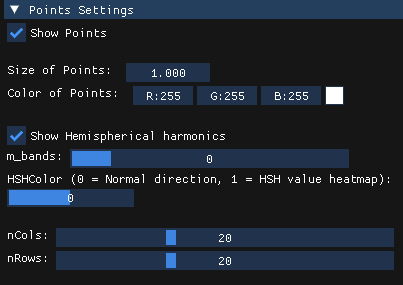
\includegraphics[width=0.475\linewidth]{obrazky-figures/UI_points.png}
    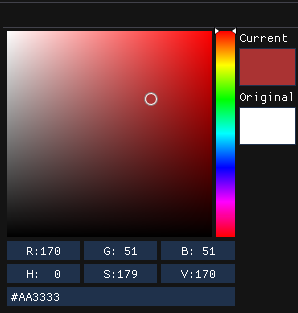
\includegraphics[width=0.32\linewidth]{obrazky-figures/UI_colorpicker.png}
    \caption{Nastavenia nad mračnami bodov a zobrazenie výberu farby}
\end{figure*}

\chapter{Implementácia}
\label{Implementacia}
Táto kapitola do hĺbky vysvetľuje jednotlivé procesy potrebné pre fungovanie programu a~algoritmy navrhnuté v~predchádzajúcej kapitole. Obsah kapitoly sa teda často odkazuje na~sekcie v~kapitolách \ref{Teoria} a \ref{Navrh}, v~ktorých sú prípadné detaily vysvetlené podrobnejšie. 
\section{Načítanie dát}
Sekcia načítanie dát sa venuje bližšiemu vysvetleniu a priblíženiu algoritmov, ktoré boli použité pri parsovaní vstupných súborov. Návrhy týchto algoritmov sú zobrazené v~sekcii \ref{DataVykreslenie}.
\subsection*{Parsovanie súboru s~mračnom bodov}
Pri parsovaní súboru s~mračnom sa najprv otvorí súbor pomocou jeho cesty a načíta sa~prvý riadok zo súboru do premennej \verb|line|. Parsovanie prebieha po jednotlivých riadkoch. Používa sa pritom metóda cyklovania \verb|while|, ktorá kontroluje hodnotu v~premennej \verb|line|. Po~prečítaní všetkých riadkov posledné volanie \verb|readline| vracia prázdny string a cyklus končí.

Hodnoty v~riadku sú oddelené medzerou alebo čiarkou. Pre zabezpečenie oboch možností sa najprv nahradia v~stringu všetky čiarky za medzery a potom sa string rozdelí podľa medzier na menšie stringy, kde každý obsahuje práve jednu hodnotu v~riadku.Hodnoty sa~ukladajú do premenných v~poradí, ako sú opísané v~návrhu v~sekcii \ref{PointCloudParse}. Pri koeficientoch HSH je parsovanie zložitejšie, keďže ich počet môže byť rozdielny podľa konkrétneho mračna bodov. Preto sa koeficienty ukladajú do generovaného zoznamu, kam sa vloží každá zvyšná hodnota v~riadku.

Po uložení všetkých hodnôt v~riadku do vektorov sa tieto vektory pripoja na poslednú pozíciu polí so všetkými hodnotami ostatných bodov v~mračne. Teda pozícia vektora v~tomto poli je rovnaká, ako pozícia riadku v~súbore. S~týmito polami sa následne pracuje ďalej v~programe. Ako posledné sa vypočíta maximálna úroveň zanorenia HSH funkcií, ktorá sa~rovná druhej odmocnine počtu koeficientov HSH v~riadku a zatvorí sa súbor.

\subsection*{Parsovanie XML}
Parsovanie XML je navrhnuté v~sekcii \ref{XMLParse}. XML súbor má formát scény v~Mitsuba renderer, ktorý je opísaný v~sekcii \ref{TeoriaMitsuba}. Pri parsovaní sa používa Python knižnica \verb|ElementTree|. Táto knižnica rozdelí XML dokument do dátových štruktúr, kde každá štruktúra znázorňuje element stromu. Tieto štruktúry sú medzi sebou prepojené rovnako ako v~elementy v~dokumente. Ako prvá vec pri parsovaní sa uloží koreňový element XML stromu do premennej.

Parsovanie prebieha prechádzaním pod-elementov koreňa stromu. Dôležité sú elementy s~tagom \verb|shape|, ktorého príklady sú ukázané v~obrázku \ref{XMLShape}. Ak sa pri kontrole tagu pod-elementu zhoduje tag s~názvom \verb|shape|, tak sa vytvorí prázdny slovník pre ukladanie informácií vnútri tohto elementu.

Atribúty elementu v~strome sú už rovno uložené v~štruktúre ako slovník, kde názov atribútu je kľúč k~hodnote atribútu. Podobne sa atribúty uložia aj do slovníka \verb|shape|. Pod-elementy, ktoré sú~dôležité, sú \verb|string| a \verb|transform|. Prvý obsahuje cestu k~.obj súboru a~druhý zase transformácie objektu.

Atribúty sa pridávajú do slovníka pod-elementu rovnako ako do \verb|shape| slovníka. V~týchto atribútoch sa napríklad nachádza cesta k~.obj súboru. Transformácie sú pod-elementy elementu \verb|transform| a sú zoradené v~poradí akom majú byť vykonané. Preto sa ukladajú do~klasického zoznamu, kde ich pozícia značí poradie operácie nad objektom.

Pod-elementy sa ku slovníkom svojich rodičovských elementov pripoja s~kľúčom, ktorý je ich tag. Finálny slovník \verb|shape| sa pripojí na koniec zoznamu \verb|Objects| s~ktorým sa pracuje ďalej v~programe.

\begin{figure*}[t!] \label{XMLShape}
    \centering
    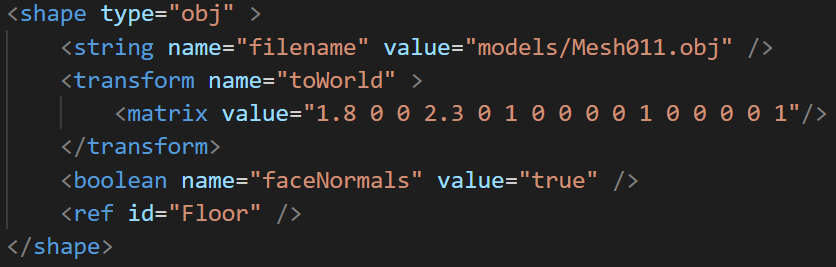
\includegraphics[width=0.58\linewidth]{obrazky-figures/XMLShape.png}
    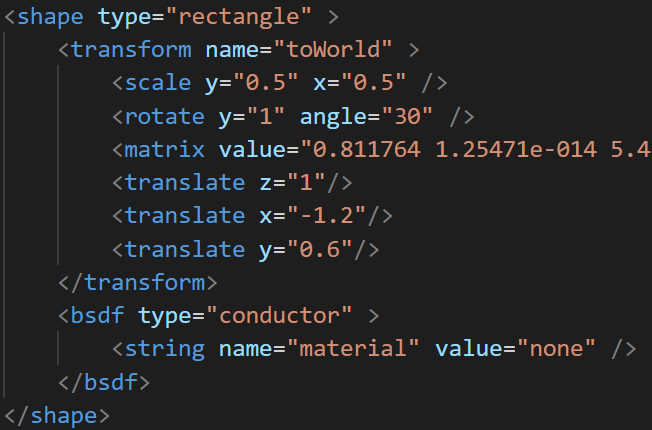
\includegraphics[width=0.40\linewidth]{obrazky-figures/XMLShape2.png}
    \caption{Príklady \texttt{shape} elementu v~XML súbore}
\end{figure*}

\subsection*{Čítanie slovníkov s~objektami v~scéne}
Objekt v~scéne môže byť typu \verb|obj|, \verb|sphere| alebo \verb|rectangle|. Pre posledné dve možnosti je cesta k~.obj súboru konštantná. Pre typ \verb|obj| je cesta jedinečná pre každý objekt a nachádza sa v~slovníku pod kľúčmi \verb|string| a \verb|value|. V~tomto prípade je dôležité pred samotnú cestu k~objektu pridať aj cestu k~XML súboru.

Ak je v~slovníku transformácia, musí sa vypočítať transformačná matica, inak je táto matica jednotková. Do funkcie na vytvorenie transformačnej matice sa posiela len zoznam s~transformáciami.

\subsection*{Tvorba transformačnej matice}
Transformačná matica začína ako jednotková matica, ktorá sa postupne násobí s~každou transformáciou. Diagram tvorby transformačnej matice je na obrázku \ref{TransMatrixDia}. Typy transformácií sú \verb|scale|, \verb|rotate|, \verb|translate| alebo už predom pripravená matica. Predpokladá sa z~formátu XML súboru, že transformácie sú zoradené v~správnom poradí a nieje treba toto poradie kontrolovať. Na tvorenie matíc pre každú operáciu a ich násobenie sa využíva knižnica \verb|pyrr|, ktorá obsahuje funkcie na prácu s~maticami pre~OpenGL.

Hodnoty, ako koordinácie $x,y,z$ alebo uhol rotácie, sú uložené v~slovníku transformácie pod ich menami. Rovnako aj typ transformácie, ktorý je uložený pod kľúčom \verb|type|. Hodnoty $x,y,z$ môžu byť aj pod kľučom \verb|value|, kde sú písané v~stringu vedľa seba oddelené čiarkami. Normálne tam bývajú všetky tri hodnoty, ale pri škálovaní môže byť len jedna hodnota. Ak~je tam len jedna hodnota, znamená to že do každej dimenzie sa objekt zväčší alebo zmenší rovnako. Pri výbere hodnôt z~\verb|value| sa rozdelí tento string podľa čiarok na tri menšie stringy, kde každý obsahuje jednu koordinačnú hodnotu. Následne sa už len tieto hodnoty vytiahnu zo stringov do pred-pripravených premenných.

Konkrétne matice transformácie sa posielajú v~stringu a parsujú sa podobne ako \verb|value|. Môžu byť vo formáte $3 \times 3$ alebo $4 \times 4$. V~prípade kratšej matice sa musí pred použitím rozšíriť o~štvrtý riadok a stĺpec. Hodnoty matice sú od seba oddelené medzerami a~je ich potrebné transponovať pred použitím v~OpenGL.

Po vynásobení jednotkovej matice všetkými operáciami sa táto matica vracia ako transformačná matica objektu.

\begin{figure*}[t!] \label{TransMatrixDia}
    \centering
    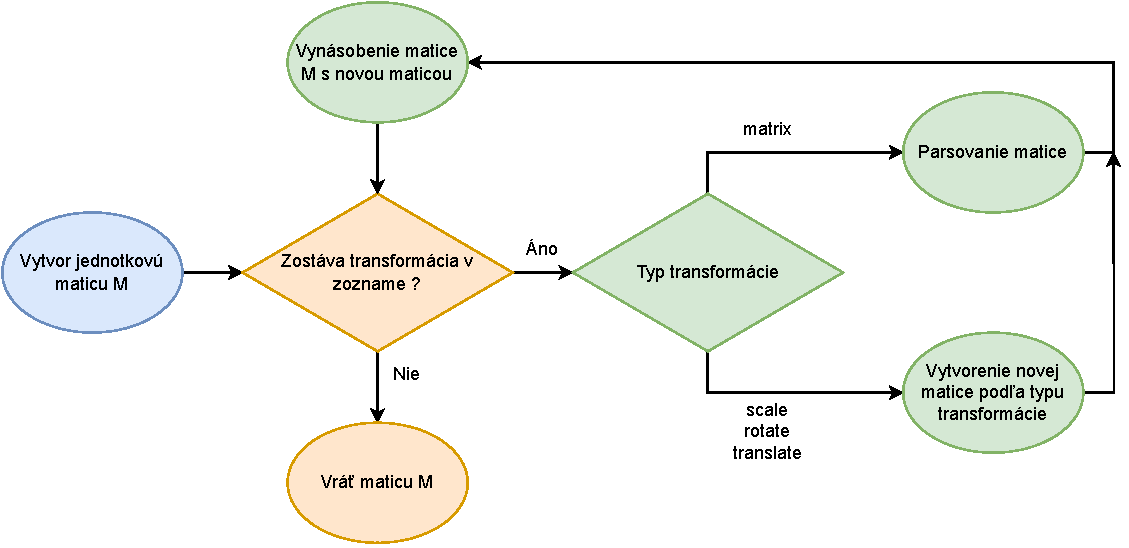
\includegraphics[width=0.90\linewidth]{obrazky-figures/TransformationMatrix.drawio.pdf}
    \caption{Diagram tvorby transformačnej matice}
\end{figure*}

\subsection*{Parsovanie .obj súboru}
Parsovanie .obj súboru prebieha podobne ako pri mračne bodov. Každý riadok sa číta samostatne a hodnoty sa ukladajú do bufferov, z~ktorých sa na konci zostaví finálny buffer so zoradenými hodnotami. Formát .obj súboru je bližšie popísaný v~sekcii \ref{OBJFormat}. Pri načítaní riadku sa skontroluje typ dát. Relevantné typy dát sú vrcholy ($v$) a zostavené primitívy~($f$). Ak~je typ dát $v$ tak sa pomocou funkcie nahrajú koordinácie vrcholu do~zoznamu \verb|coords|. Ak je typ $f$ tak sa zapíšu pozície vrcholov do~zoznamu pozícií \verb|indices|. Pseudokód parsovania .obj súboru je zobrazený v~algoritme \ref{ObjFilePseu}.

Ak sa primitív skladá z~troch vrcholov, jednoducho stačí len poradia vrcholov zapísať za sebou do \verb|indices|. Ak sa však skladá zo štyroch, treba ho rozdeliť na dva trojuholníky, ktorých vrcholy sa postupne zapíšu do zoznamu. Tieto trojuholníky za skladajú z~vrcholov 1, 2, 3 a 1, 3, 4.

Pred uložením vrcholu do bufferu sa koordinácie zmenia na float. Výsledná hodnota sa~ešte pred nahratím škáluje. Hodí sa to napríklad pri načítaní objektu pre body, ktorý je jednotková guľa. Rovno pri načítaní sa vie naškálovať na veľkosť menšieho bodu.

Pri zostavovaní finálneho zoradeného bufferu sa prechádza cez hodnoty v~zozname \verb|indices| podľa ktorých sa zistí pozícia vrcholu v~zozname \verb|coords| a vloží sa do~finálneho bufferu. Zoradený buffer a dĺžka zoznamu \verb|indices| sú vratné hodnoty, ktoré sa používajú ďalej v~programe.

\begin{algorithm}[t!]
\caption{Parsovanie .obj súboru}\label{ObjFilePseu}
\While{line = readline()}{
    \If{line.empty()}{
        $continue$    \\
    }
    $line = line.split()$ \\
    \If{line[0] == 'v'}{
        $coords.addVertex(line[1], line[2], line[3])$
    }
    \If{line[0] == 'f'}{
        \uIf{len(line[1:]) == $3$}{
        $indices.addIndices(line[1], line[2], line[3])$
        }
        \ElseIf{len(line[1:]) == $4$}{
        $indices.addIndices(line[1], line[2], line[3])$ \\
        $indices.addIndices(line[1], line[3], line[4])$
        }
    }
}
\end{algorithm}

\subsection*{Filtrovanie bodov}
\label{PointFiltering}
Návrh filtrovania bodov je v~sekcii \ref{FiltrBodovNavrh}. Na začiatku filtrovania bodov sa upraví a skopíruje buffer objektu, aby sa s~ním mohlo voľne pracovať. Potom sa pridá k~pozíciám bodov štvrtý stĺpec pre umožnenie skalárneho súčinu so $4 \times 4$ transformačnou maticou. Týmto súčinom sa vrcholy objektu transformujú na rovnaké miesto ako budú vykreslené v~scéne.

Ak sú už vrcholy na správnych miestach, je možné začať s~filtráciou. Kváder sa vytvára nájdením najväčších a najmenších hodnôt medzi vrcholmi objektu. Preto je potrebné otočiť osi v~dvojrozmernom poli. S~takto otočenými osami sú všetky hodnoty jedného typu koordinácie v~jednom poli a tak sa dá lahšie identifikovať najmenšia a najväčia hodnota. K~týmto hodnotám sa ešte pripočítava výplň, pre počítanie bodov aj v~blízkom okolí objektu.

Ako posledné sa prejde cez všetky body v~mračne a zhodnotí sa, či sa ich pozícia nachádza vnútri kvádra. Indexy bodov, ktoré sa nachádzajú dnu sa ukladajú do zoznamu, ktorý sa~využíva ďalej v~programe.

\section{Nastavenie kamery a pohyb v~priestore}
Pri vykresľovaní scény v~reálnom čase je dôležité mať možnosť pohybu kamery po scéne. Inak nieje potrebné scénu vykresľovať v~reálnom čase. Pre pohyb a zobrazenie objektov v~kamere sa používajú matice, ktoré presúvajú a deformujú objekty v~scéne pre navodenie ilúzie pohybu v~troj-dimenzionálnom priestore. Tieto matice sú matica projekcie a matica pohľadu. V~shaderi sa nimi násobia vrcholy objektov po ich umiestnení v~scéne.

\subsection*{Matica perspektívnej projekcie}
Bližšie informácie o~projekčných maticiach sú v~sekcii \ref{KameraTeoria}. Pri začatí programu sa vypočíta matica perspektívnej projekcie pre veľkosť základného okna. Používa sa pritom znova knižnica \verb|pyrr|. Funkcia \verb|create_perspective_projection| vytvára matice perspektívnej projekcie priamo použiteľné v~OpenGL. Berie štyri parametre a to uhol pohľadu v~stupňoch, pomer dĺžky a výšky obrazu a hodnoty blízkeho a vzdialenejšieho fokálneho bodu. Dĺžka a výška obrazu sa určuje v~počte pixelov okna v~ktorom sa aplikácia zobrazuje a~fokálne body určujú oblasť v~ktorej sa objekty budú zobrazovať.

Táto matica sa mení iba pri zmene rozlíšenia vykresľovacieho okna. Cez \verb|callback| funkciu, ktorá sa zavolá vždy pri zmene rozlíšenia, sa pomocou nových hodnôt vypočíta nová matica. Ak by sa nevypočítala, objekty by v~scéne vyzerali deformovane.

\subsection*{Matica pohľadu}
\label{viewmat}
Matica pohľadu slúži na určenie polohy a smeru pohľadu kamery v~scéne. Jej úloha je posúvať objekty a tým navodiť ilúziu pohybu kamery. Na jej vytvorenie slúži funkcia \verb|create_look_at| z~knižnice \verb|pyrr|. Vstupné parametre funkcie sú tri vektory. Prvý vektor je pozícia kamery v~scéne. Druhý vektor je cieľ v~scéne na ktorý sa kamera pozerá. Cieľ môže byť súčet pozície kamery a vektoru smeru otočenia kamery. Tretí vektor smeruje od~kamery nahor.

Táto matica sa generuje pri každom novom snímku, pretože ovplyvňuje pohyb po scéne. Na~začiatku render loopu sa vždy prepočítajú kamerové vektory, podľa ktorých sa vypočíta nová matica pohľadu. Táto matica sa následne nahrá do vertex shaderu ako \verb|uniform| premenná.

\begin{figure*}[b!] \label{MoveDia}
    \centering
    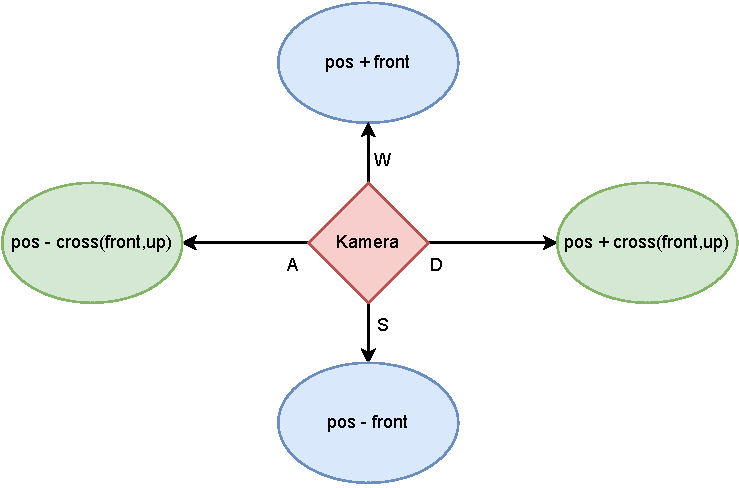
\includegraphics[width=0.60\linewidth]{obrazky-figures/CamMovement.drawio.pdf}
    \caption{Diagram pohybu kamery}
\end{figure*}

\subsection*{Pohyb po scéne}
\label{Movement}
Pohyb po scéne sa realizuje stlačením tlačítok W, A, S, D na klávesnici. Diagram pohybu kamery je na obrázku \ref{MoveDia}. Na začiatku render loopu sa volá funkcia, ktorá spracúva vstup klávesnice a myši nad vykresľovacím oknom. Pre~zachovanie konzistentnej rýchlosti pohybu kamery pri rôznych časoch vykreslenia snímky sa násobí konštanta rýchlosti s~časom medzi poslednými dvoma vykreslenými snímkami. Pri stlačení tlačítka W sa k~pozícii kamery pripočíta vektor smeru kamery vynásobený rýchlosťou pohybu. Pri stlačení S~sa zase tento výsledok odpočíta.

Pri~pohybe do strán sa vypočíta skalárny súčin vektorov smerujúcich pred a nad kameru. Vypočítaný vektor je kolmý k~obom vektorom a smeruje doprava od smeru kamery. Pri stlačení D sa teda k~pozícii kamery tento vektor pripočítava a zase pri stlačení A~odpočítava.

\begin{algorithm}[b!]
\caption{Počítanie nových vektorov kamery}\label{CameraVectorsPseu}
$jaw$ += \textit{xoffset} $* sensitivity$    \\
$pitch$ += \textit{yoffset} $* sensitivity$  \\
\If{pitch > $89.9$}{
    $pitch = 89.9$ 
}
\If{pitch < $-89.9$}{
    $pitch = -89.9$ 
}
\texttt{\\}
$camFront.x = \cos(rad(jaw)) * \cos(rad(pitch))$ \\
$camFront.y = \sin(rad(pitch))$                  \\
$camFront.z = \sin(rad(jaw)) * \cos(rad(pitch))$ \\
\texttt{\\}
$camFront = norm(camFront)$\\
$camRight = norm(camFront \times [0.0, 1.0, 0.0])$\\
$camUp = norm(camFront \times camRight)$
\end{algorithm}

\subsection*{Pohľad kamery}
Pri pohľade kamery sa upravujú vektory \verb|camera_front| a \verb|camera_up|. Pre uchovanie rozdielu polohy myšky medzi snímkami sa používa \verb|callback| funkcia, ktorá tento rozdiel počíta. Posúvanie pohľadu funguje len pri stlačení pravého tlačítka myši. Preto je potrebné kontrolovať stav tohto tlačítka pomocou boolean premennej. Ak tlačítko na myši nieje stlačené, premenná má hodnotu \verb|True| a nezaznamenáva sa rozdiel pohybu myši. Ak je stlačené tak sa správne počíta rozdiel medzi momentálnou pozíciou myši a pozíciou myši na minulom snímku. Rozdiel osi $y$ sa počíta opačne ako osi $x$ pretože rasterizácia obrazu prebieha zľava doprava, odhora dolu. Čiže veci nižšie na obrazovke majú vyššiu hodnotu $y$ ako veci vyššie. Rozdiely pozície podla osi sa uložia do premenných \verb|xoffset| a \verb|yoffset|.

Nové hodnoty vektorov sa počítajú v~metódach objektu \verb|cam|. Pseudokód výpočtu je v~algoritme \ref{CameraVectorsPseu}. Najskôr sa upravia hodnoty \verb|xoffset| a \verb|yoffset| pomocou prednastavenej senzitivity a pripočítajú sa k~\verb|jaw| a \verb|pitch|. \verb|Jaw| predstavuje pohyb sprava doľava a \verb|pitch| zhora dole. Pred výpočtom nových vektorov sa ešte skontroluje hodnota \verb|pitch| či nepresahuje priamy uhol. Ak by presahovala tak by sa kamera otočila a nefungovala by~správne.

Najprv sa vypočíta podľa vzorca vektor smeru kamery. Vektor \verb|camera_right| sa vypočíta skalárnym súčinom novo-vytvoreného \verb|camera_front| vektora a vektora smerujúceho nahor. Vektor \verb|camera_up| sa vypočíta skalárnym súčinom vektorov \verb|camera_front| a~\verb|camera_right|. Pre násobenie vektorov sa používa knižnica \verb|pyrr|. 

Tieto vektory sa ukladajú do premenných používaných v~programe vo funkcii na spracovanie vstupov, ak je stlačené pravé tlačítko myši.

\section{Reprezentácia dát na GPU}
Po načítaní dát zo vstupných súborov je dôležité tieto dáta uložiť do pamäte na grafickej karte, aby sa s~nimi dalo pracovať v~shaderoch. Táto sekcia sa venuje spôsobu uloženia dát na GPU a následnému prístupu k~nim.

\subsection*{Reprezentácia objektov}
Pre každý objekt v~scéne sa vytvorí samostatný Vertex Array Object (VAO) a Vertex Buffer Object (VBO). VAO slúži na identifikáciu VBO v~ktorom sú uložené pozície vrcholov objektu na grafickej karte. Po prepojení VBO na VAO a nastavení typu bufferu sa musí pripraviť miesto na grafickej karte a špecifikovať adresa skadiaľ sa bude do bufferu zapisovať pomocou funkcie \verb|glBufferData|. Na určenie spôsobu uloženia dát v~bufferi slúži funk-cia \verb|glVertexAttribPointer|. Parametrom tejto funkcie je aj lokácia vstupnej premennej v~shaderi s~ktorou sa bude pracovať na grafickej karte. Táto lokácia je prvým parametrom funkcie. Nasleduje počet hodnôt, ktoré patria k~sebe a typ hodnoty. Nasledujúce parametre slúžia na voľbu normalizácie hodnôt a k~prípadným skokom v~bufferi. Keďže vrcholy sú~v~zoradenom bufferi uložené tesne vedľa seba nieje potrebné tieto parametre nastavovať.

\subsection*{Reprezentácia mračna bodov}
Pre mračno bodov sa vytvoria dve VAO. Jedno slúži na objekt bodu, ktorý sa bude vykresľovať na pozíciach bodov v~mračne a druhý slúži na hemisférický objekt, ktorý sa bude deformovať pomocou HSH funkcií. Vrcholy oboch objektov sa nahrávajú rovnako ako vrcholy objektov v~scéne. Avšak je potrebné nahrať do grafickej pamäte aj posuvné matice pre zmenu pozície bodu. Tieto matice sa počítajú podobne ako posuvné matice pri skladaní transformačných matíc pre objekty. Na posun sa používa pozícia bodu v~scéne. Každá hodnota z~matice sa~následne nahrá samostatne za sebou do zoznamu.

Pri nahrávaní matice do klasického bufferu však nastáva problém a to, že parameter funkcie \verb|glVertexAttribPointer| s~množstvom hodnôt vedľa seba môže mať hodnotu maximálne štyri a matica ich má šestnásť. Samotná vstupná premenná v~shaderi však môže byť typu $4 \times 4$ matice, ale zaberá 4 lokácie. Pre každú z~týchto lokácií je potrebné zavolať funkciu \verb|glVertexAttribPointer| a pri týchto volaniach sa už naplno využije preskakovanie v~rámci bufferu. Možnosť normalizácie stále ostáva nevyužitá, ale hodnoty v~bufferi už nie sú tesne vedľa seba. Vzdialenosť od jednotlivých matíc v~bajtoch je veľkosť jednej hodnoty v~zozname krát šestnásť a začiatok čítania sa pre každý riadok matice bude posúvať o~veľkosť predchádzajúcich riadkov rovnako v~bajtoch. Keďže sa body v~mračne renderujú inštančne, pomocou funkcie \verb|glVertexAttribDivisor| sa nastaví, že matice sa budú striedať každú inštanciu.

Tieto matice sa nahrajú rovnako do oboch VAO bodov v~mračne. K~hemisférickému objektu je potrebné ešte nahrať normály, tangenty a bitangenty bodov v~mračne. Avšak keďže sú~to~znova len vektory s~troma hodnotami, nahrávajú sa podobne ako vrcholy objektu s~rozdielom nastavenia \verb|Divisor| znova na jednu inštanciu.

\subsection*{Shader Storage Buffer Object}
Do Shader Storage Buffer Object (SSBO) je možné uložiť veľké množstvo dát, ktoré sú v~rámci shader kódu vždy prístupné. Je teda vhodným miestom na uloženie pozícií a vyfiltrovaných indexov bodov pre renderovanie tepelných máp, alebo na uloženie koeficientov HSH funkcií. Ukladanie do SSBO je podobné ako do klasického bufferu. Do parametra funkcie \verb|glBindBufferBase| je potrebné zapísať binding point SSBO, ktorý symbolizuje jeho lokáciu v~shaderi.

\subsection*{Prístup k~hodnotám v~shaderi}
Nahrávané hodnoty z~bufferov sú v~shaderi uložené vo vstupných premenných. Pri deklaráciách týchto premenných sa nastavuje lokácia, ktorá sa využíva pri nahrávaní hodnôt z~bufferov. Hodnoty vo vstupných premenných sa aktualizujú vždy podľa aktuálneho vrcholu, ktorý sa vykresľuje.

SSBO vnútri shaderu vyzerá ako štruktúra v~programovacom jazyku C a k~hodnotám vnútri sa pristupuje rovnako ako ku hodnotám vnútri štruktúry. Rovnako ako pri vstupných premenných sa pri deklarácii píše aj binding point.

Transformačné matice sa ukladajú do shaderov ako \verb|uniform| hodnoty a tiež sú dostupné vždy v~rámci shader kódu.

\section{Render Loop}
Pri renderovaní v~reálnom čase sa musí pre každý snímok vykresliť scéna samostatne. Ak je týchto snímkov dostatočne veľa za sekundu, navádza to ilúziu pohybu. Snímky sa vykresľujú v~nekonečnom cykle do okna programu. Tento cyklus sa volá render loop a jeho diagram je v~obrázku \ref{RLDia}.

\subsection*{Inicializácia pred render loopom}
Pred samotným render loopom je potrebné inicializovať okno, do ktorého sa bude scéna renderovať. Okno sa inicializuje pomocou knižnice \verb|glfw|, ktorá je priamo určená na použitie pri renderovaní pomocou OpenGL. Po vytvorení a určení pozície na obrazovke sa pre okno určí kontext. Znamená to, že príkazy grafickej knižnice sa budú vykonávať nad týmto oknom.

Užívatelské rozhranie je riešené cez knižnicu \verb|ImGUI|, ktorú treba rovnako inicializovať a~vytvoriť objekt \verb|Renderer|, ktorý vykreslí okno užívateľského rozhrania do \verb|glfw| okna.

\begin{figure*}[b!] \label{RLDia}
    \centering
    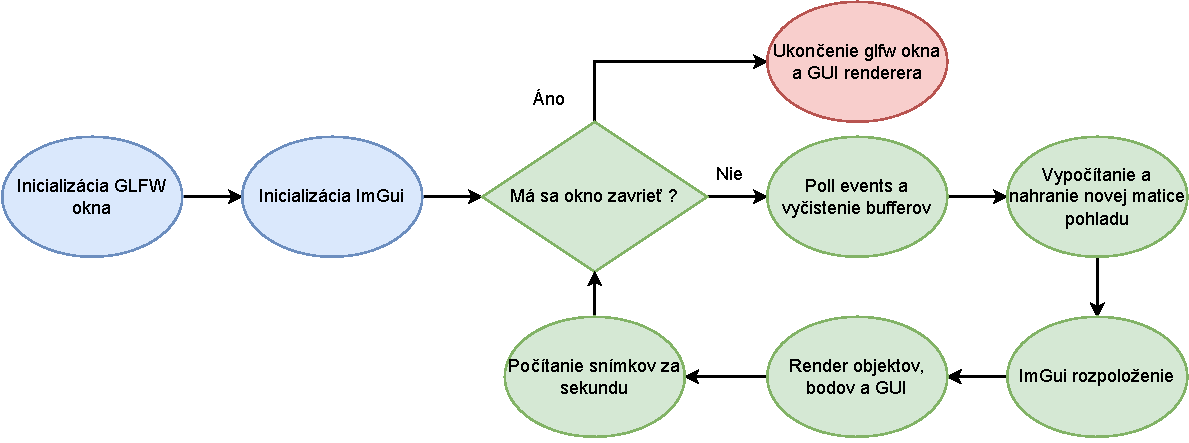
\includegraphics[width=0.95\linewidth]{obrazky-figures/RenderLoop.drawio.pdf}
    \caption{Diagram pohybu kamery}
\end{figure*}

\subsection*{Vnútri render loopu}
Pre render loop je ideálne použiť cyklus typu \verb|while|. Aj keď je to nekonečný cyklus, keď sa užívateľ rozhodne zatvoriť program, mal by prestať prebiehať aj render scény. V~\verb|glfw| knižnici preto existuje funkcia \verb|window_should_close|, ktorá vracia \verb|True| ak sa užívateľ rozhodol zavrieť okno. Na začiatku render loopu sa zhromaždia všetky udalosti pomocou funkcie \verb|poll_events|. V~tejto funkcii sa zaznamenajú všetky interakcie s~klávesnicou a~myšou a zavolajú sa \verb|callback| funkcie. Potom sa vyčistia bufferi a upravia sa vektory kamery podľa postupu v~sekcii \ref{viewmat}.

Po vypočítaní a nahratí novej matice pohľadu do shaderu sa určuje podoba užívatelského rozhrania a renderujú sa objekty, body v~scéne a užívatelské prostredie. Po renderi sa~vypočíta trvanie vykreslenia snímky a podľa tohto času sa vypočíta počet snímkov za~sekundu. Po skončení \verb|while| cyklu treba korektne ukončiť \verb|Renderer| užívateľského rozhrania a zavrieť okno.

\section{Inštančné renderovanie bodov a HSH funkcií}
\label{HSHImpl}
Táto sekcia opisuje implementáciu renderovania bodov z~mračna a HSH funkcií. Návrh implementácie HSH funkcií je v~sekcii \ref{HSHNavrh} a teória k~týmto funkciám je v~sekcii \ref{HSHlabel}.

\subsection*{Renderovanie bodov v~mračne}
Renderovanie bodov v~mračne je v~tomto bode, kedy sú už všetky hodnoty nahrané v~grafickej pamäti, celkom jednoduché. V~kóde programu sa nastaví prepínač v~shaderi na~renderovanie mračna bodov pomocou zmeny jeho hodnoty v~\verb|uniform| premennej. Následne sa naviaže VAO objektu bodu na renderovanie. Inštančné renderovanie sa spúšťa funkciou \verb|glDrawArraysInstanced|. Táto funkcia má 4 parametre, a to spôsob renderovania, začiatočný index vrcholu, počet vrcholov a počet inštancií. Spôsob renderovania je uložený v~premennej \verb|RenderType|, pretože je volený užívateľom. Typy používané v~aplikácii sú \verb|GL_LINES| a \verb|GL_TRIANGLES|, ktoré vykresľujú len čiary medzi vrcholmi alebo aj vnútra trojuholníkov.

Kód vnútri shaderov je tiež jednoduchý a pozostáva len z~vypočítania pozície vrcholu na~obrazovke a uloženia farby bodu. Vo fragment shaderi sa len táto farba vrcholu vloží do~fragmentu.

\subsection*{Generovanie hemisférického objektu}
Pseudokód generovania hemisférického objektu je vložený v~algoritme \ref{HemGenPseu}. Najprv sa musia pre hemisférický objekt vygenerovať vrcholy. Vrcholy sa generujú pomocou dvoch uhlov. Uhol $\theta$ znázorňuje vektor smeru a jeho hodnota v~radiánoch je v~rozsahu $[0, 2\pi]$. Uhol $\phi$ znázorňuje výšku a jeho hodnota v~radiánoch je v~rozsahu $[0, \frac{\pi}{2}]$. Podľa vzorca sa pomocou týchto uhlov vypočíta pozícia vrcholu, ktorá sa pridá do zoznamu s~ostatnými vrcholmi. Riadkov sa počíta o~jeden viac pretože je potrebné vygenerovať vrcholy aj pre úplne vrchný riadok.

Podobne ako pri načítaní .obj súboru, je potrebné vytvoriť buffer v~ktorom sú zoradené vrcholy do trojuholníkov. Tu je však potrebné si poradie vrcholov vkladaných do bufferu vypočítať. Keď sa pri počítaní príde na koniec riadku, poradie vrcholu vedľa je rovné prvému vrcholu v~tom riadku. Preto je potrebné tieto hodnoty upraviť aby sa nepresiahol objem pola pri ukladaní do bufferu.

Po vytvorení bufferu sa tento buffer nahrá do VAO hemisférického objektu a môže sa s~ním ďalej pracovať.

\begin{algorithm}[t!]
\caption{Generovanie hemisférického objektu}\label{HemGenPseu}
$vertices = []$ \\
\For{(i = 0; i < nRows + 1; i++)}{
    $\theta = \frac{i}{nRows} * \frac{\pi}{2}$ \\
    \For{(j = 0; i < nCols; j++)}{
        $\phi = \frac{j}{nCols} * 2\pi$ \\
        $x = \cos(\phi) * \sin(\theta)$ \\
        $y = \cos(\theta)$              \\
        $z = \sin(\phi) * \sin(\theta)$ \\
        $vertices.addVertex(x, y, z)$
    }
}
\texttt{\\}
$buffer = []$\\
\For{(i = 0; i < nRows; i++)}{
    \For{(j = 0; i < nCols; j++)}{
        $v0 = i * nCols + j$        \\
        $v1 = v0 + 1$               \\
        $v2 = (i + 1) * nCols + j$  \\
        $v3 = v2 + 1$               \\
        \If{$v1\mod nCols == 0$}{
            $v1$ = $v1 - nCols$ \\
            $v3$ = $v3 - nCols$ \\
        }
        \texttt{\\}        
        $buffer.addTriangle(v0, v1, v2)$ \\
        $buffer.addTriangle(v2, v1, v3)$
    }
}
\end{algorithm}

\subsection*{Vytvorenie matice modelu pre bod}
Matica modelu slúži na orientáciu pologule v~smere normálu bodu. Vytvára sa vynásobením matice s~pozíciou bodu s~maticou obsahujúcou tangentu, bitangentu a normál bodu. Rovnica \ref{ModelMatrixforHSH} zobrazuje tento výpočet.

\begin{equation} \label{ModelMatrixforHSH}
    M = 
    \begin{pmatrix}
    1 & 0 & 0 & 0\\
    0 & 1 & 0 & 0\\
    0 & 0 & 1 & 0\\
    pos.x & pos.y & pos.z & 1
    \end{pmatrix}
    \cdot
    \begin{pmatrix}
    t.x & t.y & t.z & 0\\
    b.x & b.y & b.z & 0\\
    n.x & n.y & n.z & 0\\
    0 & 0 & 0 & 1
    \end{pmatrix}
\end{equation}

\subsection*{Určenie pozície vrcholu na pologuli}
Pred určením presnej polohy je potrebné identifikovať obdĺžnik na pologuli kde sa vrchol nachádza. Keďže je pologuľa generovaná, je známy počet vrcholov podľa počtu stĺpcov a~riadkov. S~týmito informáciami sa dá presne určiť poloha obdĺžnika. Obrázok \ref{Polgul} ukazuje pologuľu rozloženú na obdĺžniky pre lepšiu predstavu.

\begin{figure*}[t!]\label{Polgul}
    \centering
    
\includegraphics[width=0.90\linewidth]{obrazky-figures/polgul.png}
    \caption{Pologuľa rozdelená na obdĺžniky}
\end{figure*}

Poloha vrcholu sa počíta rovnako ako pri generovaní hemisférického objektu a znázorňujú ju 2 uhly $\theta$ a $\phi$. Podľa stĺpca a riadka vrcholu sa vypočíta normalizovaná hodnota týchto uhlov, ktorá sa prevedie do radiánov. Hodnota HSH funkcie sa počíta s~použitím týchto uhľov a indexom vykresľovanej inštancie \verb|shID|.

\subsection*{Výpočet hodnoty HSH na vrchole}
Hodnota HSH sa počíta podľa vzorcov v~sekcii \ref{ShiftedALP} a pseudokód jej výpočtu je v~algoritme \ref{VypocetHSHpseu}. Pri výpočtoch sa používajú posunuté asociované Legendreove polynómy. V~premennej \verb|m_bands| je maximálna úroveň zanorenia do koeficientov HSH a je ovládaná užívateľom. Čím je táto hodnota vyššia, tým je náročnejší výpočet na grafiku. Koeficienty z~SSBO sa získavajú vo funkcii \verb|coef|, kde sa vyberajú podľa poradia inštancie a pozícií zanorenia koeficientu \verb|l| a \verb|m|.

\begin{algorithm}[b!]
\caption{Výpočet HSH funkcie}\label{VypocetHSHpseu}
$result = 0$\\
\For{(l = 0; l < m\_bands; l++)}{
    \For{(m = 1; m $\leq$ l; m++)}{
       $L = \Tilde{P}^m_l(\cos\theta) * \Tilde{K}^m_l(\cos(m\phi))$ \\
       $result $ += $ coef(shID, l, -m) * \sqrt{2} * \sin(m\phi) * L$ \\
       $result $ += $ coef(shID, l, +m) * \sqrt{2} * \cos(m\phi) * L$ \\
    }
    $result $ += $ coef(shID, l, 0) * \Tilde{P}^0_l(\cos\theta) * \Tilde{K}^0_l(\cos(m\phi))$ \\
}
\end{algorithm}

\subsection*{Deformácia a zafarbenie vrcholu}
Poloha vrcholu sa znova vypočíta s~použitím uhlov $\theta$ a $\phi$ pre zaistenie, že vypočítaná hodnota HSH sa nanesie na správnu pozíciu na hemisfére. Táto poloha sa vynásobí výsledkom z~HSH funkcie a upraví sa škálovaním hemisférového objektu čím sa deformuje do žiadanej pozície.

Vrchol môže byť zafarbený dvoma spôsobmi. Prvý spôsob je farba podľa normálu vrcholu a druhý spôsob je tepelná mapa podľa hodnoty HSH funkcie. Normál vrcholu sa nenahráva do shaderu a preto je ho potrebné vypočítať pomocou sčítania inverznej a transponovanej matice modelu s~pozíciou vrcholu. Rovnica \ref{NormalHSHColor} zobrazuje tento výpočet. Hodnotu farby je potrebné pred použitím normalizovať.

\begin{equation} \label{NormalHSHColor}
Color = (M^{-1})^T \cdot (verPos, 1)
\end{equation}

Jednoduchá tepelná mapa podľa HSH hodnoty prechádza zo zelenej farby v~bode, ktorý je deformovaný negatívne, ku červenej farbe v~bode, ktorý bol deformovaný pozitívne. Aby sa~zmenila farba zo zelenej na červenú, musí sa odčítať hodnota \verb|g| a pripočítať hodnota \verb|r| v~rgb vektore. Ak sa budú tieto hodnoty upravovať výsledkom HSH funkcie vznikne tepelná mapa medzi zelenou a červenou na základe HSH hodnoty. Rovnica \ref{HMHSHColor} zobrazuje tento výpočet. Farbu je potrebné pred použitím normalizovať.

\begin{equation} \label{HMHSHColor}
Color = (|HSH|, 1.0 - |HSH|, 0.0)
\end{equation}

\begin{figure*}[t!]\label{HSHshading}
    \centering
    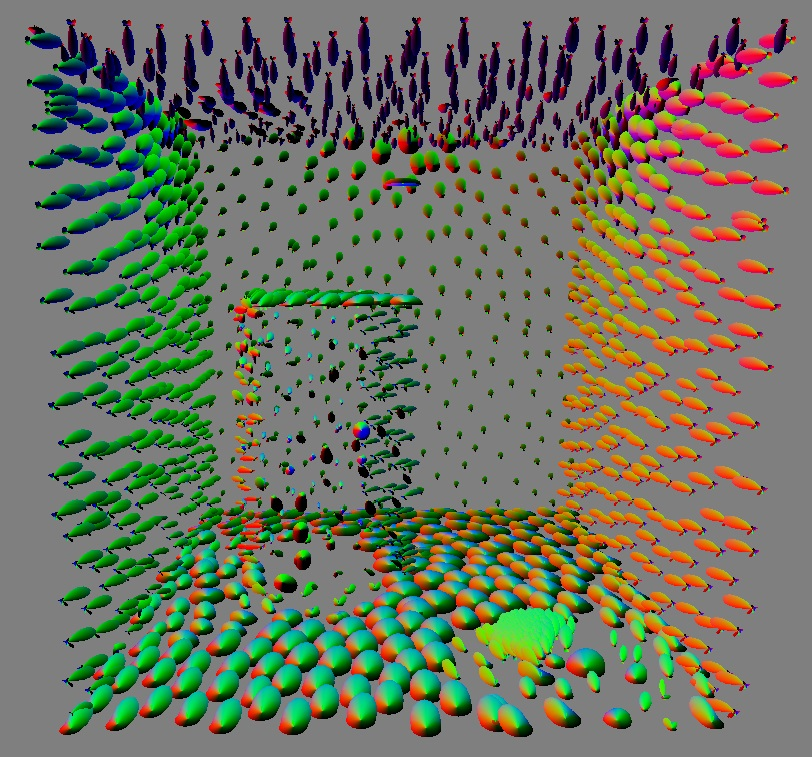
\includegraphics[width=0.45\linewidth]{obrazky-figures/normalshading.jpg}
    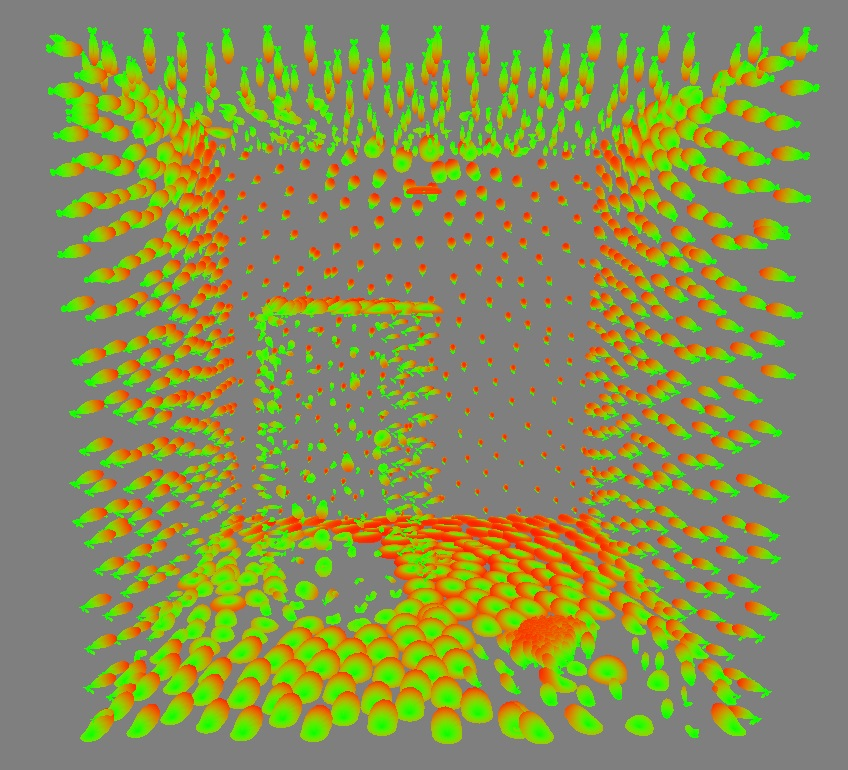
\includegraphics[width=0.46\linewidth]{obrazky-figures/HSHshading.jpg}
    \caption{Ukážky farbenia HSH funkcií}
\end{figure*}

\noindent Oba spôsoby zafarbenia sú zobrazené na obrázku \ref{HSHshading}.

\section{Renderovanie objektov a tepelnej mapy}
Táto sekcia sa zaoberá spôsobom implementácie renderovania objektov v~scéne a zafarbenia týchto objektov tepelnou mapou. Návrh renderovania tepelných máp je opísaný v~sekcii \ref{HMNavrh} a teória o~tepelných mapách sa nachádza v~sekcii \ref{HMlabel}.

\subsection*{Renderovanie objektov bez tepelnej mapy}
\label{SceneImpl}
Aby bolo možné rozlíšiť objekty v~scéne od seba, musia byť rozdielne zafarbené. Preto sa~pre každý objekt sa vytvorí náhodný odtieň farby od bielej po modrú. Tieto farby boli vybrané, pretože nie sú príliš nápadné a zároveň sú lahko rozlíšiteľné.

Po parsovaní .obj súboru sa pre každý objekt vygeneruje pseudonáhodné číslo od $0$~do~$1$. Toto číslo sa následne odčíta od \verb|r| a \verb|g| hodnôt jednotkového vektoru, ktorý sa potom nahrá do zoznamu vektorov na pozíciu totožnú s~pozíciou objektu. Toto znamená, že ak je pseudonáhodné číslo nízke, farba objektu je bližšie k~bielej. Čím je číslo väčšie, tým je farba objektu modrejšia.

Vnútri render loopu sa v~cykle pre každý objekt naviaže VAO, kde sú uložené zoradené vrcholy objektu. Pred renderom je potrebné nahrať maticu modelu a farbu modelu do~\verb|uniform| premenných v~shaderi. Vykreslenie objektu sa spúšťa funkciou \verb|glDrawArrays|, ktorá má tri vstupné parametre. Prvým je spôsob renderovania, čiže či sa budú vyfarbovať len čiary medzi vrcholmi alebo celé trojuholníky. Ďalšie dva sú prvý index vrcholu a počet vrcholov v~zoradenom bufferi.

Vnútri shader kódu sa pomocou matíc vypočíta pozícia vrcholu na obrazovke a nastaví sa~farba vrcholu na farbu objektu. Scéna vykreslená bez tepelnej mapy je na obrázku \ref{scenaBlue}.

\begin{figure*}[t!]\label{scenaBlue}
    \centering
    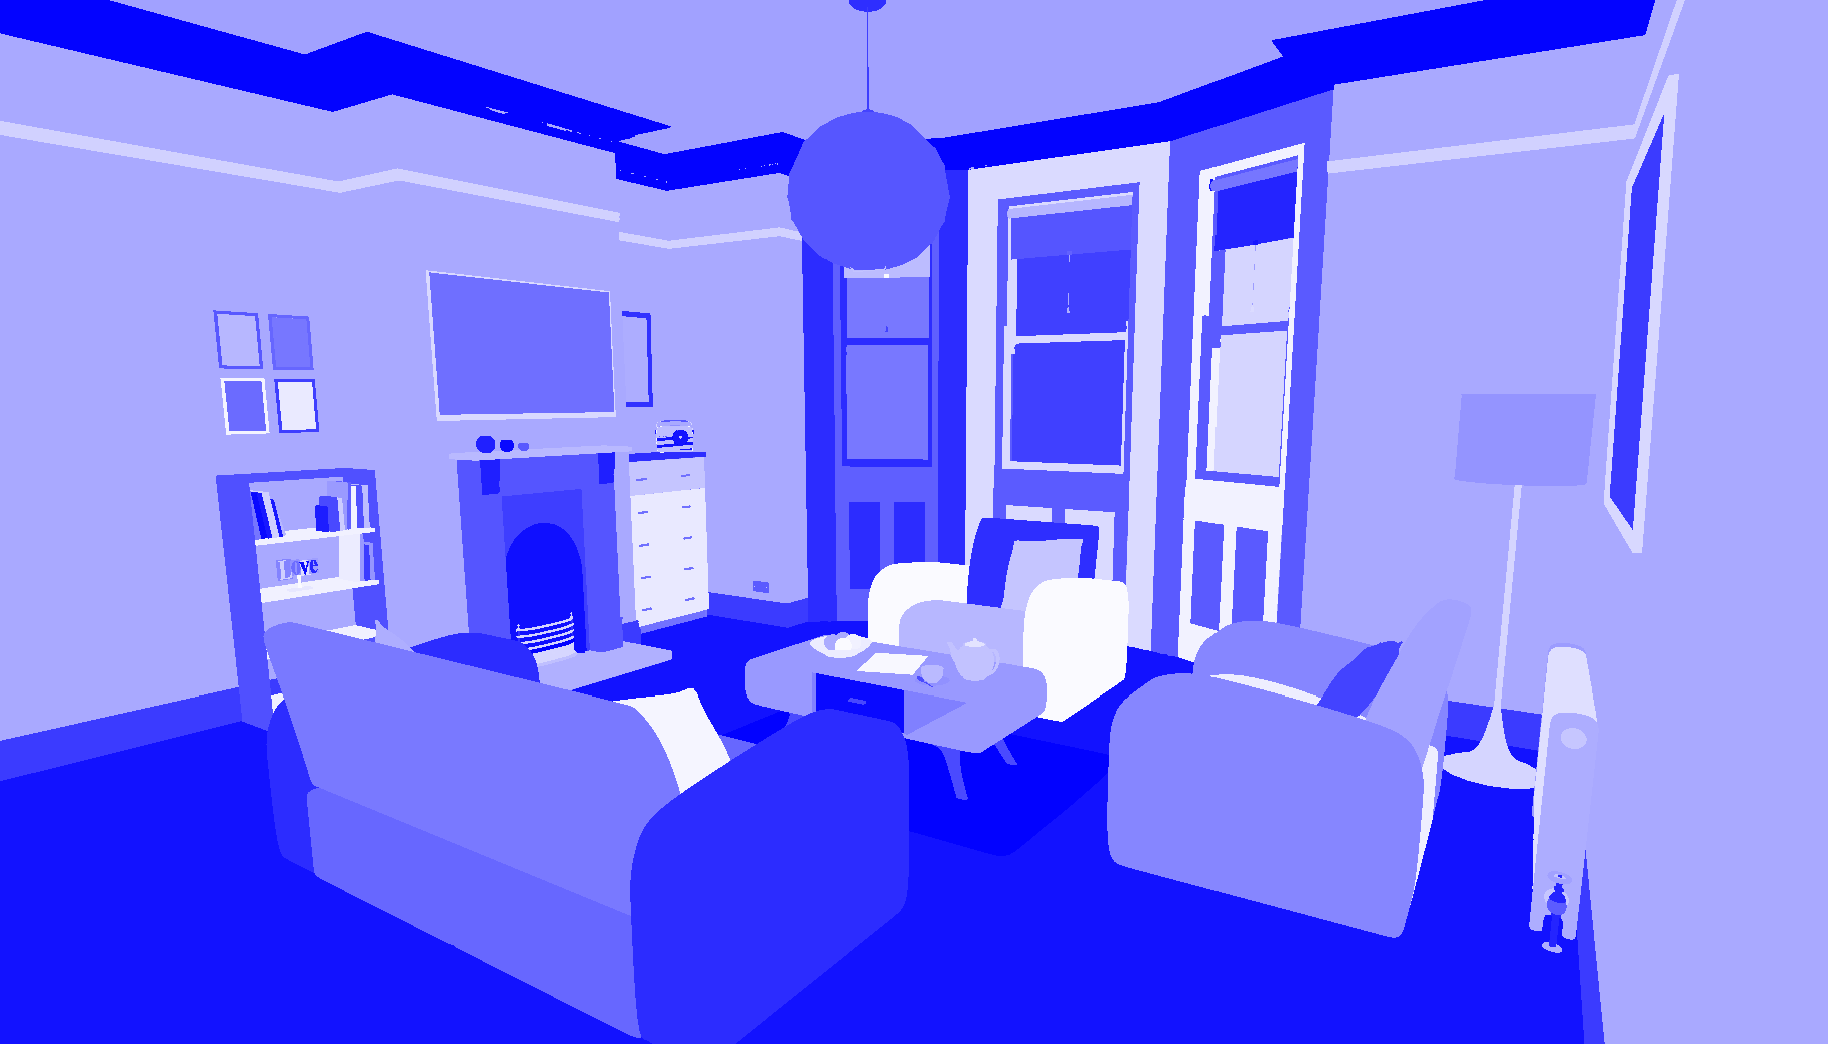
\includegraphics[width=0.80\linewidth]{obrazky-figures/scenaBlue.png}
    \caption{Scéna vykreslená v~aplikácii bez tepelnej mapy}
\end{figure*}

\subsection*{Dáta ukladané do SSBO}
Pri počítaní tepelných mapách sa používajú dve SSBO. V~prvom sú pozície všetkých bodov v~mračne zoradené za sebou a v~druhom sú prefiltrované indexy bodov, ktoré sa nachádzajú vnútri objektov. Každý objekt v~scéne má vlastnú zbierku týchto indexov a preto sú tieto zbierky zoradené za sebou v~jednom bufferi podľa poradia vykresľovaných objektov. Pomocou týchto indexov sa pri počítaní tepelnej mapy vyberajú koordinácie bodov z~prvého SSBO.

\subsection*{Renderovanie tepelnej mapy}
\label{HMImpl}
V~render loope je postup podobný ako pri renderovaniu bez tepelnej mapy. Je však potrebné nahrať do \verb|uniform| premenných v~shaderi dve hodnoty naviac. Prvá hodnota je počet bodov vnútri objektu v~zozname \verb|NobjectPoints|. Druhá hodnota je \verb|offset| a znázorňuje počet bodov vnútri objektov, ktoré boli vykreslené skorej.

Vnútri shader kódu sa najprv vypočíta hodnota tepelnej mapy v~konkrétnej pozícii na~objekte. Pomocou filtrovaných indexov bodov v~mračne sa~prejde cez každý bod, ktorý sa~nachádza v~blízkosti objektu. Vzdialenosť bodu v~mračne s~pozíciou na objekte sa vydelí maximálnou povolenou vzdialenosťou aby sa normalizovala pre následné porovnávanie. Efekt bodu na zafarbenie sa počíta pomocou vzorca $\frac{1-dis}{intensity}$. V~princípe ak je bod vzdialený má minimálny efekt a ak je blízko má efekt 1. Tento efekt sa ešte delí intenzitou tepelnej mapy určenou užívateľom.

Farba sa určuje gradientom medzi farbami podľa vypočítanej hodnoty tepelnej mapy. Ak je hodnota v~rozsahu $[0,1]$ gradient je~od bielej k~modrej, aj je v~rozsahu $[1,2]$ gradient je~od~modrej k~zelenej a ak v~rozsahu $[2,\infty]$ gradient je medzi zelenou a červenou. Hodnoty nad tri sa zobrazujú tiež ako červená farba. Pseudokód výpočtu tepelnej mapy je v~algoritme \ref{VypocetHMpseu}. Scéna vykreslená s~tepelnou mapou je na~obrázku~\ref{tepelnamapaScena}.

\begin{figure*}[t!]\label{tepelnamapaScena}
    \centering
    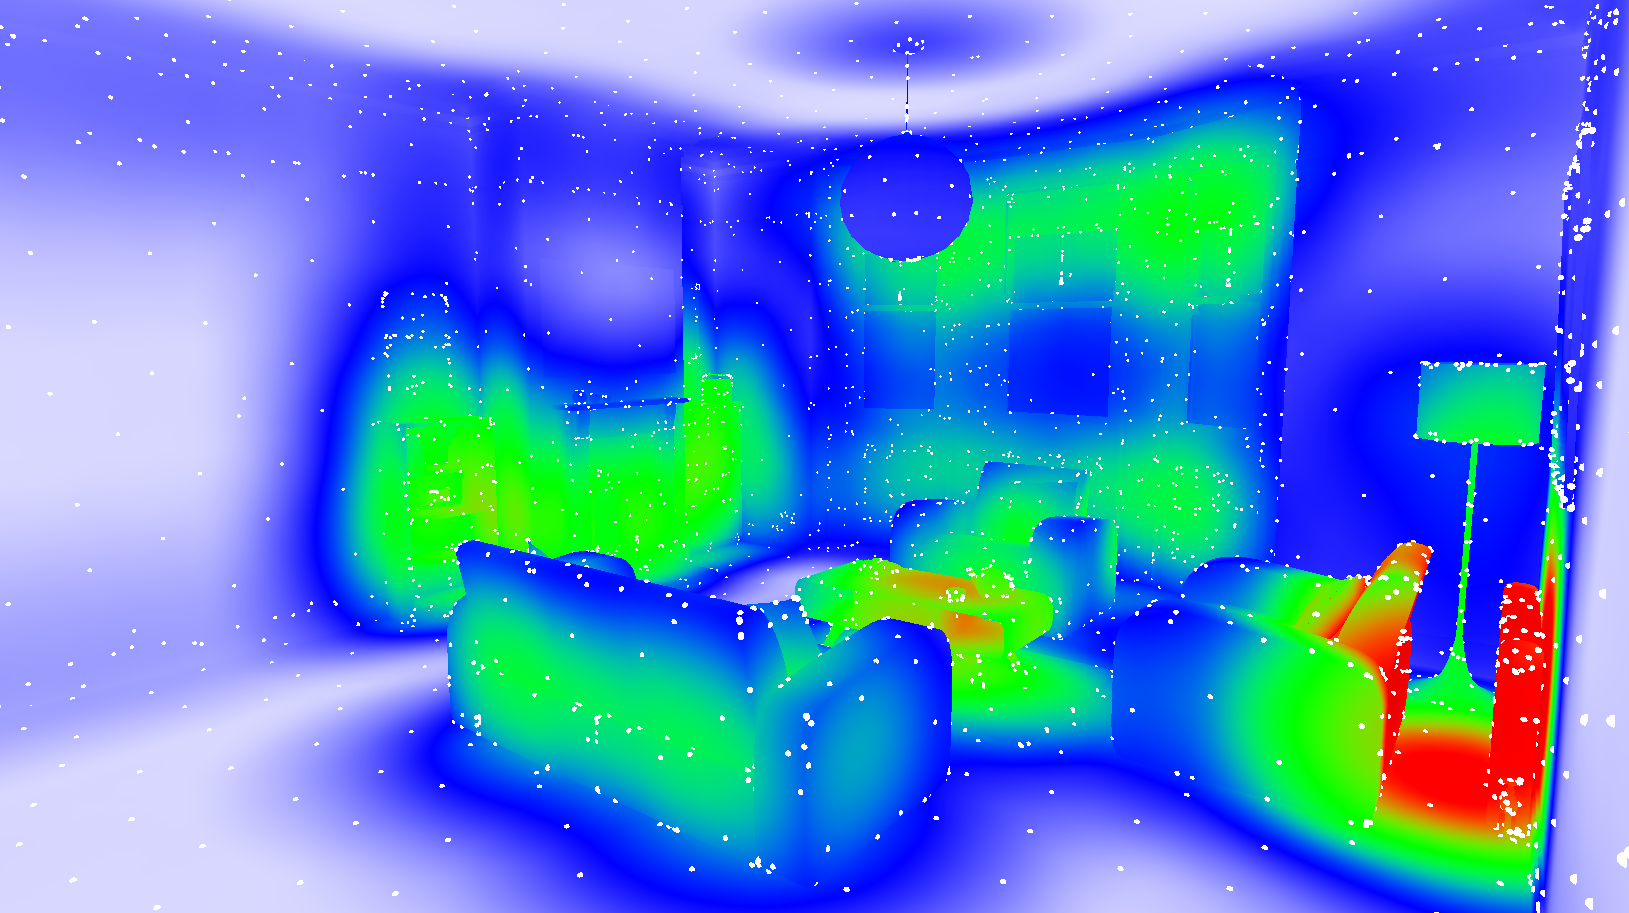
\includegraphics[width=0.90\linewidth]{obrazky-figures/tepelnamapa.png}
    \caption{Scéna vykreslená v~aplikácii s~tepelnou mapou}
\end{figure*}

\begin{algorithm}[b!]
\caption{Výpočet tepelnej mapy}\label{VypocetHMpseu}
\For{(i = offset; i < offset + NPointsIn; i++)}{
    $point = pointPos[objectPoints[i]]$ \\
    $dis = distance(verPos, point) / MaxDistance$     \\
    \texttt{\\}
    \If{dis $\leq$ 1.0}{
        $color\_cor$ += $\frac{1-dis}{intensity}$\\
    }
}
\uIf{$color\_cor < 1.0$}{
    $color = vec3(1.0 - color\_cor, 1.0 - color\_cor, 1)$ \\
}
\uElseIf{$color\_cor < 2.0$}{
    $color\_cor = color\_cor - 1$ \\
    $color = vec3(0.0, color\_cor, 1.0 - color\_cor)$ \\
}
\Else{
    $color\_cor = color\_cor - 2$ \\
    $color = vec3(color\_cor, 1.0 - color\_cor, 0.0)$ \\
}
\end{algorithm}

\section{Ovládanie / GUI}
Táto sekcia sa venuje implementácii ovládania aplikácie a grafického užívateľského rozhrania. Návrh užívateľského rozhrania je v~sekcii \ref{UINavrh}. Implementuje sa pomocou knižnice \verb|ImGui|, ktorá umožňuje vkladať hodnoty upravené užívateľom do premenných programu. 

Knižnica obsahuje funkcie, ktoré vykresľujú elementy ako posuvníky, input políčka, zaškrtávacie políčka (checkbox) alebo tlačítka. Vratné hodnoty z~týchto funkcií sú konkrétne hodnoty, ktoré boli zapísané užívateľom a boolean hodnota, ktorá značí zmenu zapísanú užívateľom. Celé GUI je na obrázku \ref{GUI}.

\subsection*{Načítanie ciest vstupných súborov}
Po zvolení cesty ku vstupnému súboru sa pred začatím parsovania skontroluje formát súboru. Pri XML sa kontroluje, či knižnica na čítanie XML dokáže prečítať súbor. Ak ho nedokáže prečítať, tak súbor nieje well-formed a teda sa nemôže použiť pri parsovaní. Pri súbori s~mračnom bodov sa kontroluje prvý riadok súboru. Ak sa úspešne prečíta tak~sa~predpokladá že celý súbor je v~poriadku.

Po skontrolovaní súborov sa nastavia boolean premenné \verb|validPC| a \verb|validXML| na hodnotu podľa toho či súbor prešiel kontrolou alebo nie. Načítavanie dát zo súborov sa vykoná len v~prípade, že hodnoty v~týchto premenných sú \verb|True|. Aplikácia vie načítať aj len objekty alebo len mračno bodov. Niektoré funkcie však budú nedostupné. \verb|Padding distance| sa vkladá priamo do premennej pre výplň vo funkcii na filtrovanie bodov v~sekcii \ref{PointFiltering}. Po načítaní vstupných súborov sa nastavia boolean premenné \verb|SceneLoaded| a \verb|CloudLoaded|. Bez toho aby tieto premenné boli v~hodnote \verb|True| sa nezobrazia objekty v~scéne. Pri uvoľňovaní dát sa tiež uvoľnia len dáta, ktoré sú načítané pomocou týchto premenných.

\subsection*{Základné nastavenia scény}
\begin{figure*}[t!]\label{GUI}
    \centering
    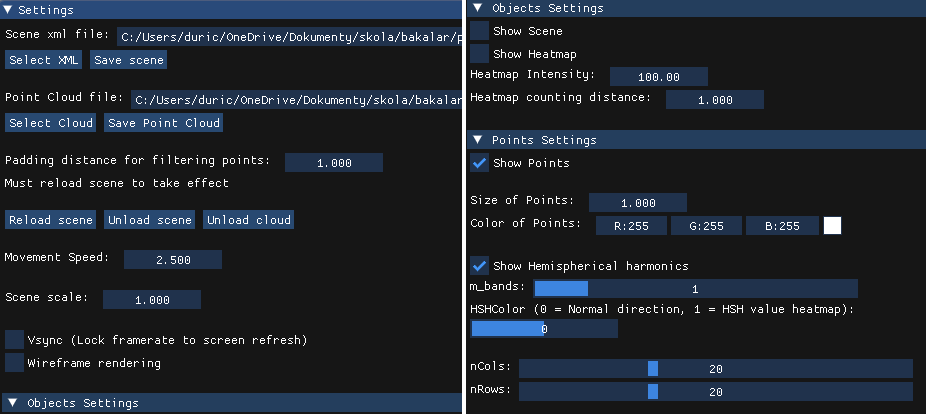
\includegraphics[width=0.95\linewidth]{obrazky-figures/GUI2.png}
    \caption{GUI aplikácie}
\end{figure*}

Základné nastavenia scény sú nastavenia, ktoré sa vzťahujú na všetky objekty na scéne, alebo na scénu samotnú. Hodnota \verb|Movement Speed| sa priamo posiela do funkcie na počítanie pozície a pohľadu kamery v~sekcii \ref{Movement}. Hodnota škálovania sa posiela do shadera pomocou \verb|uniform| premennej. Z~tejto hodnoty sa zostaví matica škálovania, ktorá je pred maticou modelu pri počítaní pozície vrcholu na obrazovke. 

Ak je checkbox \verb|Vsync| zaškrtnutý spustí sa funkcia  \verb|glfw.swap_interval(1)|. Parameter funkcie značí koľko refreshov displeja má čakať \verb|glfw| na zmenu snímku. Ak je to 0, snímka sa~po~renderovaní hneď vykreslí. Ak je to 1, ako v~tomto prípade, čaká sa na refresh monitora na vykreslenie snímky. Checkbox \verb|Wireframe| mení hodnotu v~premennej \verb|RenderType| viditeľnej v~sekciách \ref{HSHImpl} a \ref{SceneImpl}. V~tejto premennej sa nachádza typ vykreslovania primitívov v~OpenGL a teda makrá \verb|GL_LINES| a \verb|GL_TRIANGLES|. Ak je použité makro \verb|GL_LINES| tak~sa~vykresľujú len čiary medzi vrcholmi viditelné v~obrázku \ref{WireframeScene}.

\begin{figure*}[t!]\label{WireframeScene}
    \centering
    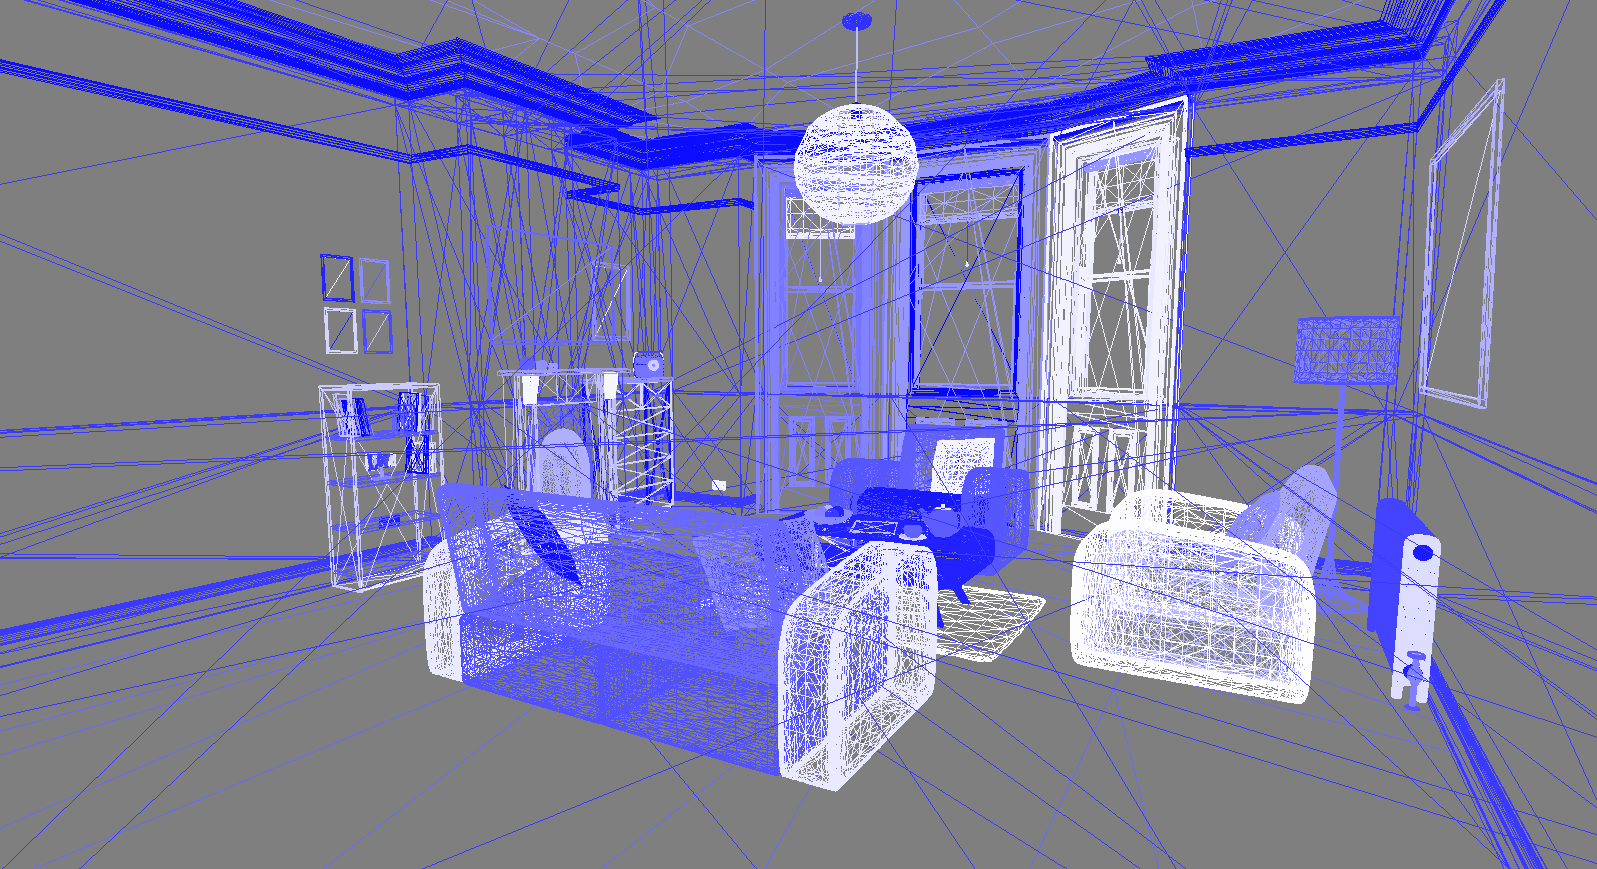
\includegraphics[width=0.90\linewidth]{obrazky-figures/wireframeScene.png}
    \caption{Wireframe render scény}
\end{figure*}

\begin{figure*}[b!]\label{Intenzita}
    \centering
    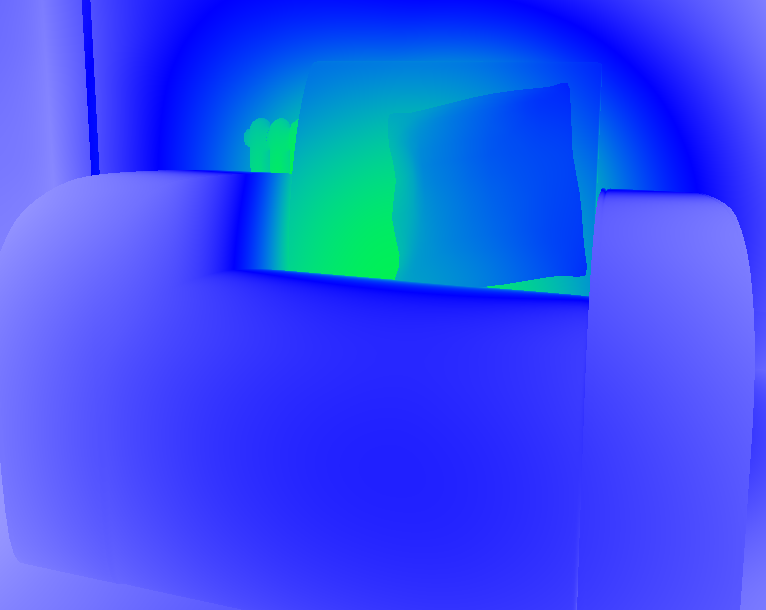
\includegraphics[width=0.45\linewidth]{obrazky-figures/int100.png}
    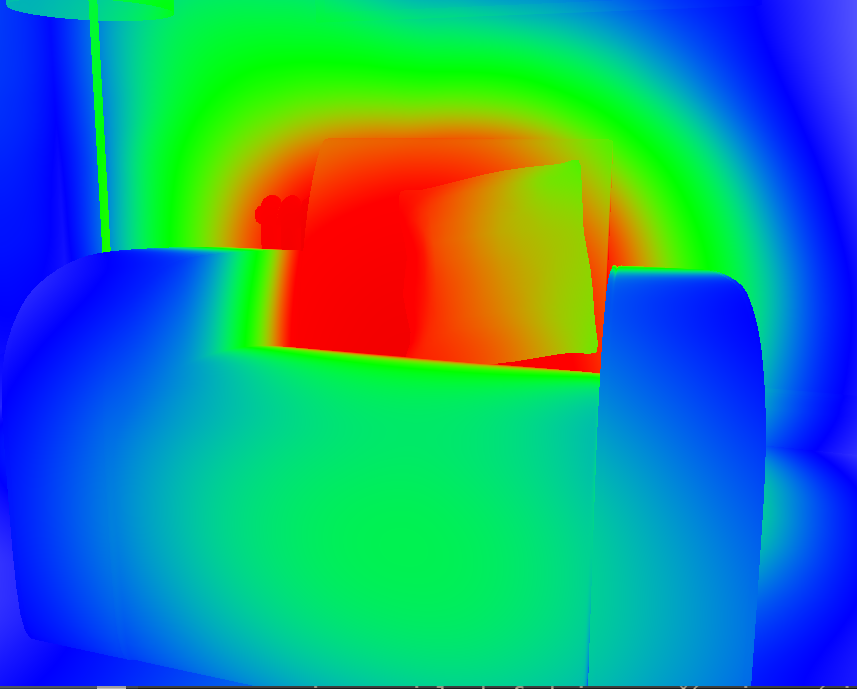
\includegraphics[width=0.45\linewidth]{obrazky-figures/int50.png}
    \caption{Rozdiel medzi intenzitou tepelnej mapy 100 a 50}
\end{figure*}

\subsection*{Nastavenia objektov tepelných máp} 
Objekty sa zobrazujú len v~prípade ak checkbox \verb|Show Scene| je zaškrtnutý. Bez zaškrtnutia \verb|Show Heatmap| sa zobrazuje scéna zafarbená odtieňmi modrej. Ak sa zaškrtne zobrazuje sa nad objektami tepelná mapa. Intenzita a vzdialenosť počítania sa posiela do \verb|uniform| premenných v~shaderi a používajú sa v~kóde v~sekcii \ref{HMImpl}. Čím je hodnota intenzity menšia, tým je efekt bodu na zafarbenie väčší. Je to kvôli tomu že sa týmto číslom delí základná hodnota efektu bodu. Rozdiel medzi intenzitami tepelnej mapy je na obrázku \ref{Intenzita}.


\subsection*{Nastavenia mračna bodov}
Zobrazovanie bodov funguje rovnako ako zobrazovanie bodov. Mračno sa zobrazí ak~sa~zaškrtne \verb|Show points|. Ak chce užívateľ zobraziť hemisférické funkcie, musia byť zaškrtnuté oba checkboxy. Veľkosť bodu sa posiela do \verb|uniform| premennej v~shaderi s~ktorou sa násobí poloha vrcholu pri počítaní jeho pozícia na obrazovke alebo polomer HSH funkcie. Rovnako aj farba bodu sa posiela do shadera ako \verb|uniform| a používa sa na zafarbenie vrcholu objektu bodu. Kód pri ktorom sa tieto \verb|uniform| premenné používajú je v~sekcii \ref{HSHImpl}.

\subsection*{Nastavenia hemisférických funkcií}
Posuvník \verb|m_bands| posiela hodnotu do \verb|uniform| premennej, ktorá určuje počet cyklov vo~\verb|for| cykle pri počítaní hodnoty HSH. Čím je hodnota vačšia, tým sa pre každý vrchol hemisféry počíta s~väčším zanorením koeficientov a zobrazenie funkcie je tým pádom presnejšie. Kód kde sa táto premenná používa je v~sekcii \ref{HSHImpl}. Rozdiel medzi úrovňami \verb|m_bands| je na~obrázku~\ref{mBands}. Typ zafarbenia HSH funkcií je v~posuvníku \verb|HSHColor| kde na 0 zafarbuje podľa smeru normálu a na 1 podľa hodnoty HSH funkcie na vrchole. Tiež sa to posiela do shaderu ako \verb|uniform| premenná. Obrázok, ktorý zobrazuje rozdiel medzi týmito zafarbeniami je obrázok~\ref{HSHshading} v~sekcii \ref{HSHImpl}.

Keď sa zmení počet stĺpcov a riadkov v~posuvníkoch \verb|nCols| a \verb|nRows|, vygeneruje sa nový hemisférový objekt s~týmto počtom stĺpcov a riadkov. Generovanie hemisférového objektu je opísané v~sekcii \ref{HSHImpl}. 

\begin{figure*}[b!]\label{mBands}
    \centering
    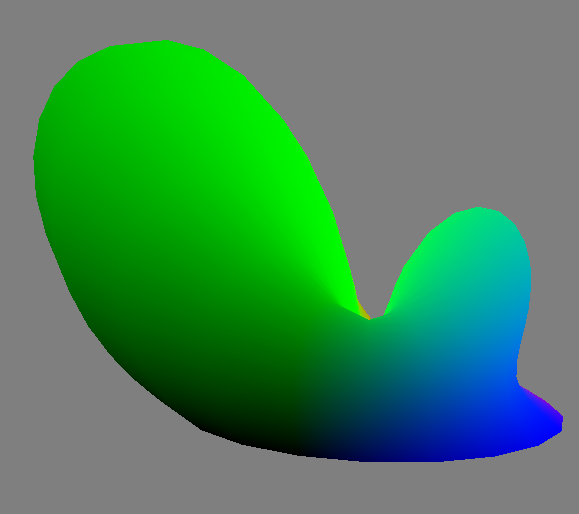
\includegraphics[width=0.48\linewidth]{obrazky-figures/mBands3.png}
    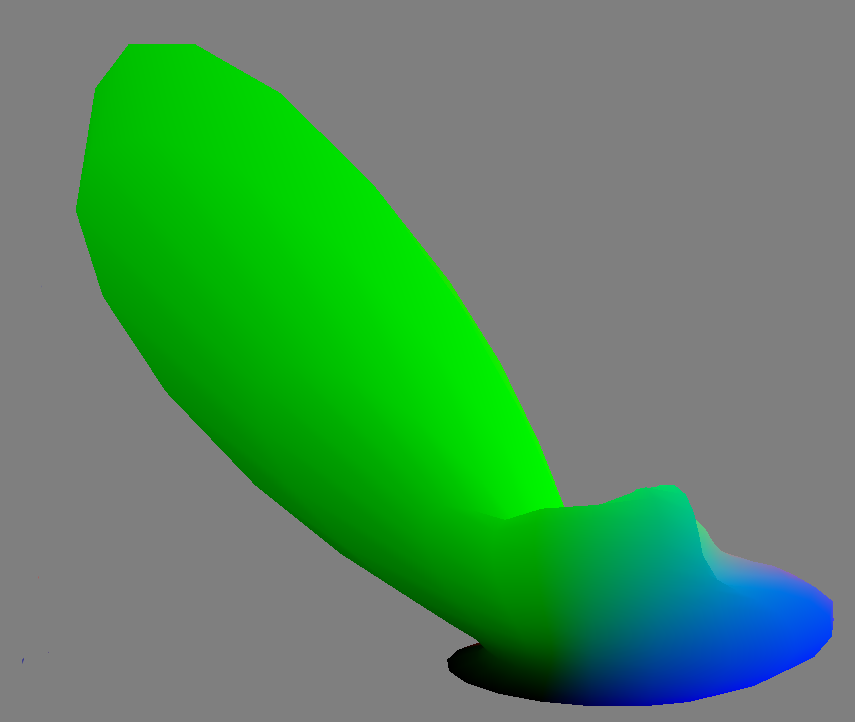
\includegraphics[width=0.50\linewidth]{obrazky-figures/mband_6.png}
    \caption{Rozdiel medzi \texttt{m\_bands} 3 a 6 pri HSH}
\end{figure*}

\section{Testovanie}
Táto sekcia sa venuje testovaniu implementácie funkcií aplikácie. Testovanie bolo vykonané na počítači s~procesorom AMD Ryzen 5 5600H a s~grafickou kartou NVIDIA RTX 3060 mobile. Informácie o~testovaných scénach sú v~tabuľke \ref{SceneDetail}.

\begin{table}[h!] \label{SceneDetail}
\centering
\begin{tabular}{|l|c|c|}
\hline
\textbf{Scéna} & \textbf{Počet objektov} & \textbf{Počet bodov v~mračne}   \\ \hline
\textit{kitchen} & 292 & 8123 \\ \hline
\textit{cornel box} & 8 & 1792 \\ \hline
\textit{living room} & 185 & 5246 \\ \hline
\textit{spaceship} & 92 & 15934 \\ \hline
\textit{staircase} & 27 & 1421 \\ \hline
\textit{veach-ajar} & 22 & 4771 \\ \hline
\textit{veach-bidir} & 14 & 1998 \\ \hline
\end{tabular}
\caption{Detaily testovaných scén}
\end{table}

\subsection*{Načítanie dát}
Tabuľka \ref{LoadingTimes} obsahuje časy načítania jednotlivých častí scén. Časy, ktoré sú v~tabuľke, sú~aritmetickým priemerom piatich meraní pre zaručenie presnosti a zamedzenie anomálií. Každý načítaný objekt v~scéne má rozdielny počet vrcholov a teda aj rozdielny čas načítania. Toto môže byť jeden z~faktorov, prečo sa niektoré scény s~menším počtom objektov načítavajú dlhšie. Ďalší zaujímavý údaj je čas načítania mračna bodov v~scéne \verb|spaceship|. Keďže každý bod má rovnaký počet hodnôt v~riadku, predpokladá sa že rozdiel v~časoch bude lineárne stúpať podľa počtu bodov v~mračne. V~tomto prípade je to však až príliš veľký rozdiel. Je možné, že vzniká spomalenie pri kopírovaní polí interpretom jazyka \mbox{Python} počas vkladania nových hodnôt. Časy filtrovania bodov celkom zodpovedajú časom načítania objektov a počtom bodov v~mračne.
\begin{table}[h!] \label{LoadingTimes}
\centering
\begin{tabular}{|l|c|c|c|c|}
\hline
\textbf{Scéna} & \textbf{Body} & \textbf{Objekty} & \textbf{Filtrovanie} & \textbf{Spolu}   \\ \hline
\textit{kitchen} & 0,652 & 3,977 & 2,436 & \textbf{7,065}\\ \hline
\textit{cornel box} & 0,079 & 0,096 & 0,029 & \textbf{0,204} \\ \hline
\textit{living room} & 0,292 & 1,774 & 0,916 & \textbf{2,982} \\ \hline
\textit{spaceship} & 3,236 & 1,559 & 1,339 & \textbf{6,134} \\ \hline
\textit{staircase} & 0,070 & 0,102 & 0,040 & \textbf{0,212} \\ \hline
\textit{veach-ajar} & 0,350 & 1,043 & 0,182 & \textbf{1,575} \\ \hline
\textit{veach-bidir} & 0,094 & 0,039 & 0,033 & \textbf{0,166} \\ \hline
\end{tabular}
\caption{Trvanie načítania scén v~sekundách}
\end{table}
\subsection*{Testovanie tepelných máp}
Tabuľka \ref{HMFPS} znázorňuje počet snímkov za sekundu pri vykresľovaní scén pri žiadnej tepelnej mape ($\varnothing$), pri tepelnej vykreslenej na vrcholoch (V) a pri tepelnej mape vykreslenej na fragmentoch (F) na rôznych rozlíšeniach. Snímky za sekundu boli vypočítané počítaním vykreslených snímkov behom piatich sekúnd a následným vydelením počtu snímkov s~prejdeným časom. Všetky hodnoty boli počítané na rovnakom mieste v~scéne a s~rovnakými nastaveniami tepelnej mapy. Tepelná mapa vykreslená na fragmentoch má viac políčok v~tabuľke pretože väčšie rozlíšenie znamená viac fragmentov pre ktorých je potrebné tepelnú mapu vypočítať. Čím viac fragmentov je teda na obrazovke, tým je výpočet mapy náročnejší. Pri vykreslení na vrcholoch sa počet vrcholov v~scéne nemení a preto nieje potrebné mať viac políčok v~tabuľke. Výkon tohto typu tepelnej mapy sa takmer nemení pri zmene rozlíšenia.

\begin{figure*}[b!]\label{PorovnanieMap}
    \centering
    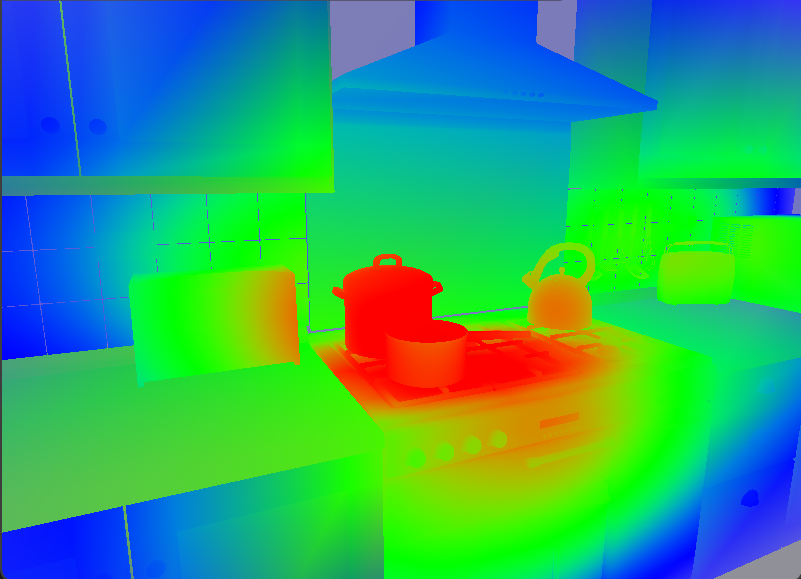
\includegraphics[width=0.48\linewidth]{obrazky-figures/VertexHM.png}
    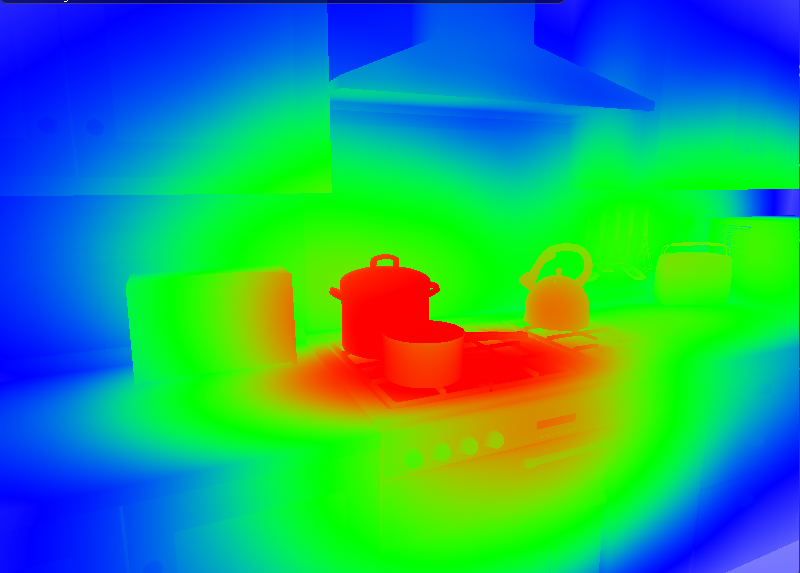
\includegraphics[width=0.485\linewidth]{obrazky-figures/FragmentHM.png}
    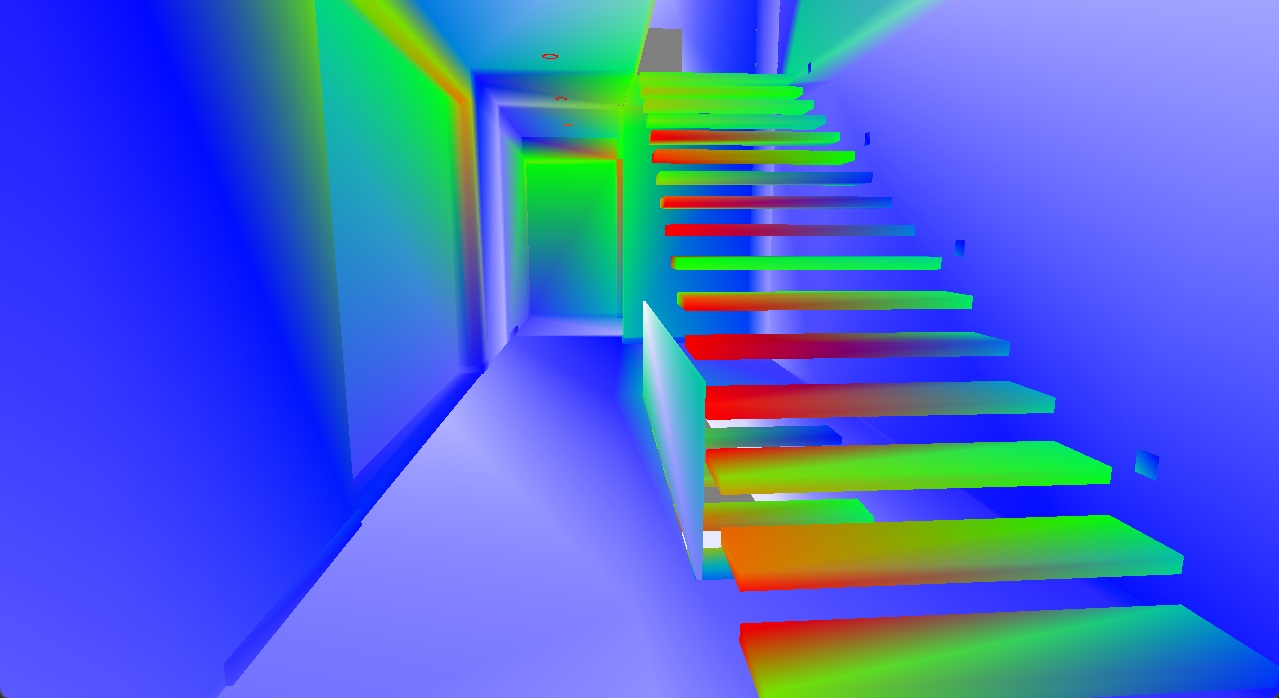
\includegraphics[width=0.48\linewidth]{obrazky-figures/VertexHM2.jpg}
    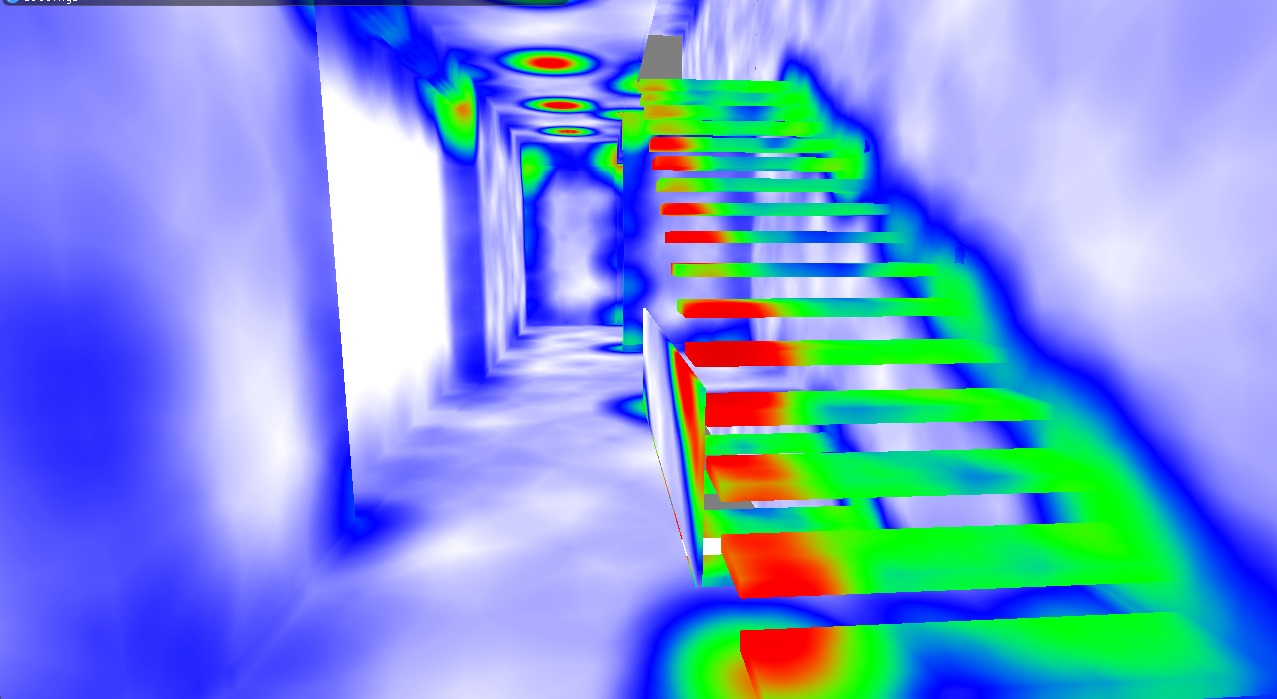
\includegraphics[width=0.48\linewidth]{obrazky-figures/FragmentHM2.jpg}
    \caption{Rozdiel medzi farbením tepelnej mapy na vrchol (vľavo) a na fragment (vpravo)}
\end{figure*}

\begin{table}[t!] \label{HMFPS}
\centering
\begin{tabular}{|l|c|c|c|c|c|}
\hline
\textbf{Scéna} & $\varnothing$ & \textbf{V} & \textbf{F(1920x1080)} & \textbf{F(1280x720)} & \textbf{F(800x600)}   \\ \hline
\textit{kitchen} & 183,338 & 18,767 & 10,441 & 14,616 & 27,869 \\ \hline
\textit{cornel box} & 788,406 & 821,493 & 169,259 & 353,969 & 499,285 \\ \hline
\textit{living room} & 249,655 & 89,472 & 9,739 & 19,91 & 39,224 \\ \hline
\textit{spaceship} & 393,77 & 17,18 & 6,995 & 13,668 & 21,642 \\ \hline
\textit{staircase} & 650,74 & 715,719 & 42,779 & 90,189 & 174,087 \\ \hline
\textit{veach-ajar} & 679,519 & 198,158 & 12,776 & 27,654 & 50,598 \\ \hline
\textit{veach-bidir} & 760,449 & 768,991 & 25,927 & 58,198 & 105,662 \\ \hline
\end{tabular}
\caption{Snímky za sekundu pri rôznych módoch tepelnej mapy}
\end{table}

\noindent Tepelná mapa farbená na fragmentoch je presnejšia ako tepelná mapa farbená na vrcholoch. Zároveň je však náročnejšia na grafiku pri vyšších rozlíšeniach. Výkon sa pri tepelnej mape na~vrcholoch sa rozlíšením nemení a preto je vhodnejšia pri vyšších rozlíšeniach. Na~obrázkoch \ref{PorovnanieMap} sú znázornené rozdiely medzi módmi vykreslenia tepelnej mapy. Čím je počet vrcholov na objektoch vyšší. tým je presnejšia aj tepelná mapa vykreslená na vrcholoch avšak tepelná mapa na fragmentoch bude vždy presnejšia. Ak sa objekt skladá z~mála trojuholníkov tepelná mapa na vrcholoch nieje presná vôbec, keďže sa farby interpolujú medzi fragmentami na celom objekte. Takisto z~týchto interpolovaných farieb môžu vznikať ostatné farby ako fialová alebo žltá, ktorá by sa nemala vykresľovať. 
\subsection*{Testovanie hemisférických funkcií}
V~tabuľke \ref{HSHFPS} sú znázornené počty snímkov za sekundu pri vykreslovaní HSH funkcií na~rôznych scénach a na rôznych úrovniach zanorenia HSH funkcií. Počítanie snímkov za sekundu prebiehalo podobne ako pri tepelných mapách. Úroveň zanorenia znázorňuje počet koeficientov použitých pri počítaní HSH funkcie. Čím viac koeficientov HSH funkcie je použitých pri počítaní, tým je render funkcie presnejší. HSH funkcie boli vykreslované na~pologuli s~15~stĺpcami a 15 riadkami. Obrázok \ref{HSHPorovnane} ukazuje rozdiely medzi jednotlivými úrovňami zanorenia funkcie. Hodnoty sú zľava doprava od 1 do 6.

\begin{table}[h!] \label{HSHFPS}
\centering
\begin{tabular}{|l|c|c|c|c|c|c|}
\hline
\textbf{Scéna} &$l \leq 1$ & $l \leq 2$ & $l \leq 3$ & $l \leq 4$ & $l \leq 5$ & $l \leq 6$   \\ \hline
\textit{kitchen} & 180,671 & 176,672 & 146,179 & 56,643 & 27,051 & 15,113 \\ \hline
\textit{cornel box} & 790,585 & 790,165 & 654,988 & 257,625 & 123,251 & 68,038 \\ \hline
\textit{living room} & 249,673 & 248,603 & 219,576 & 85,372 & 41,187 & 23,091 \\ \hline
\textit{spaceship} & 247,067 & 182,011 & 79,332 & 29,844 & 14,257 & 7,879 \\ \hline
\textit{staircase} & 657,413 & 649,275 & 645,888 & 311,391 & 149,704 & 81,638 \\ \hline
\textit{veach-ajar} & 702,713 & 573,983 & 250,216 & 94,586 & 46,221 & 25,38 \\ \hline
\textit{veach-bidir} & 759,331 & 727,195 & 604,242 & 222,989 & 106,85 & 58,195 \\ \hline
\end{tabular}
\caption{Snímky za sekundu pri úrovniach zanorenia hemisférických funkcií}
\end{table}

V~ďalšej tabuľke \ref{HSGFPS} sú zobrazené snímky za sekundu pri rôznych počtoch stĺpcov a~riadkov hemisféry na ktorej sa zobrazuje HSH funkcia. Počet riadkov a stĺpcov určuje počet vrcholov objektu s~ktorými sa bude počítať HSH funkcia. Čím väčší počet vrcholov, tým je výpočet na grafiku náročnejší ale výsledná vykreslená funkcia presnejšia. Na obrázku \ref{HSGPorovnanie} sú zobrazené tri nastavenia kvality hemisféry. Prvé je minimálna hodnota $5 \times 5$, druhé je $25 \times 25$ a posledné je maximálna hodnota $50 \times 50$.

\begin{table}[h!] \label{HSGFPS}
\centering
\begin{tabular}{|l|c|c|c|c|c|}
\hline
\textbf{Scéna} & $\textbf{10} \times \textbf{10}$ & $\textbf{20} \times \textbf{20}$ & $\textbf{30} \times \textbf{30}$ & $\textbf{40} \times \textbf{40}$ & $\textbf{50} \times \textbf{50}$ \\ \hline
\textit{kitchen} & 181,195 & 87,326 & 40,840 & 23,843 & 15,518 \\ \hline
\textit{cornel box} & 809,878 & 396,454 & 185,53 & 108,111 & 69,351 \\ \hline
\textit{living room} & 243,091 & 133,124 & 62,772 & 35,995 & 23,395 \\ \hline
\textit{spaceship} & 159,322 & 46,893 & 21,652 & 12,411 & 8,112 \\ \hline
\textit{staircase} & 668,287 & 483,074 & 227,052 & 128,49 & 82,758 \\ \hline
\textit{veach-ajar} & 491,597 & 147,819 & 68,692 & 39,561 & 26,058 \\ \hline
\textit{veach-bidir} & 786,9 & 348,775 & 162,905 & 92,307 & 59,616 \\ \hline
\end{tabular}
\caption{Snímky za sekundu pri rôznych kvalitách hemisférového objektu}
\end{table}

\begin{figure*}[t!]\label{HSHPorovnane}
    \centering
    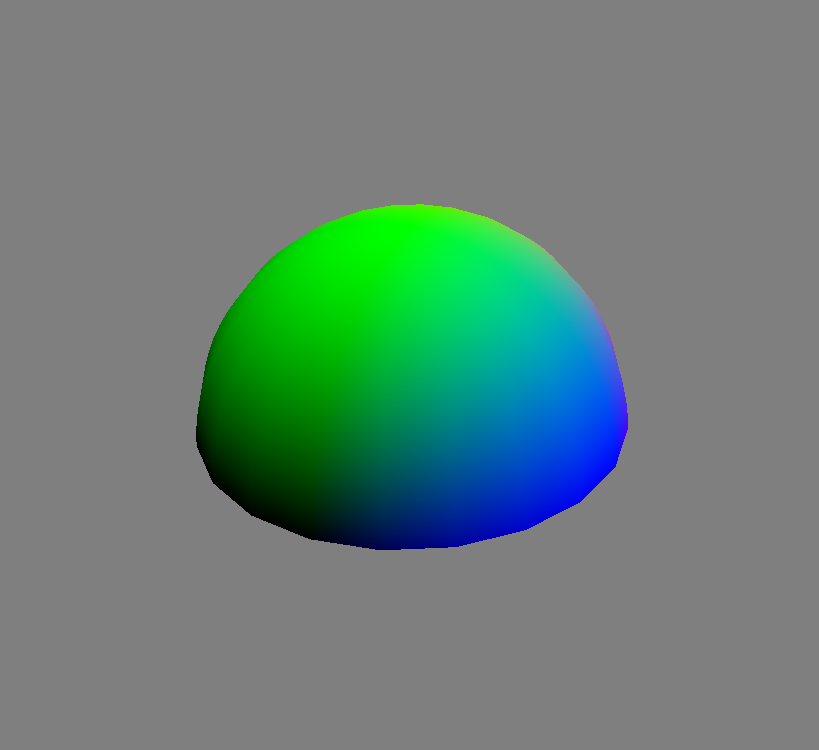
\includegraphics[width=0.245\linewidth]{obrazky-figures/HSH1.png}
    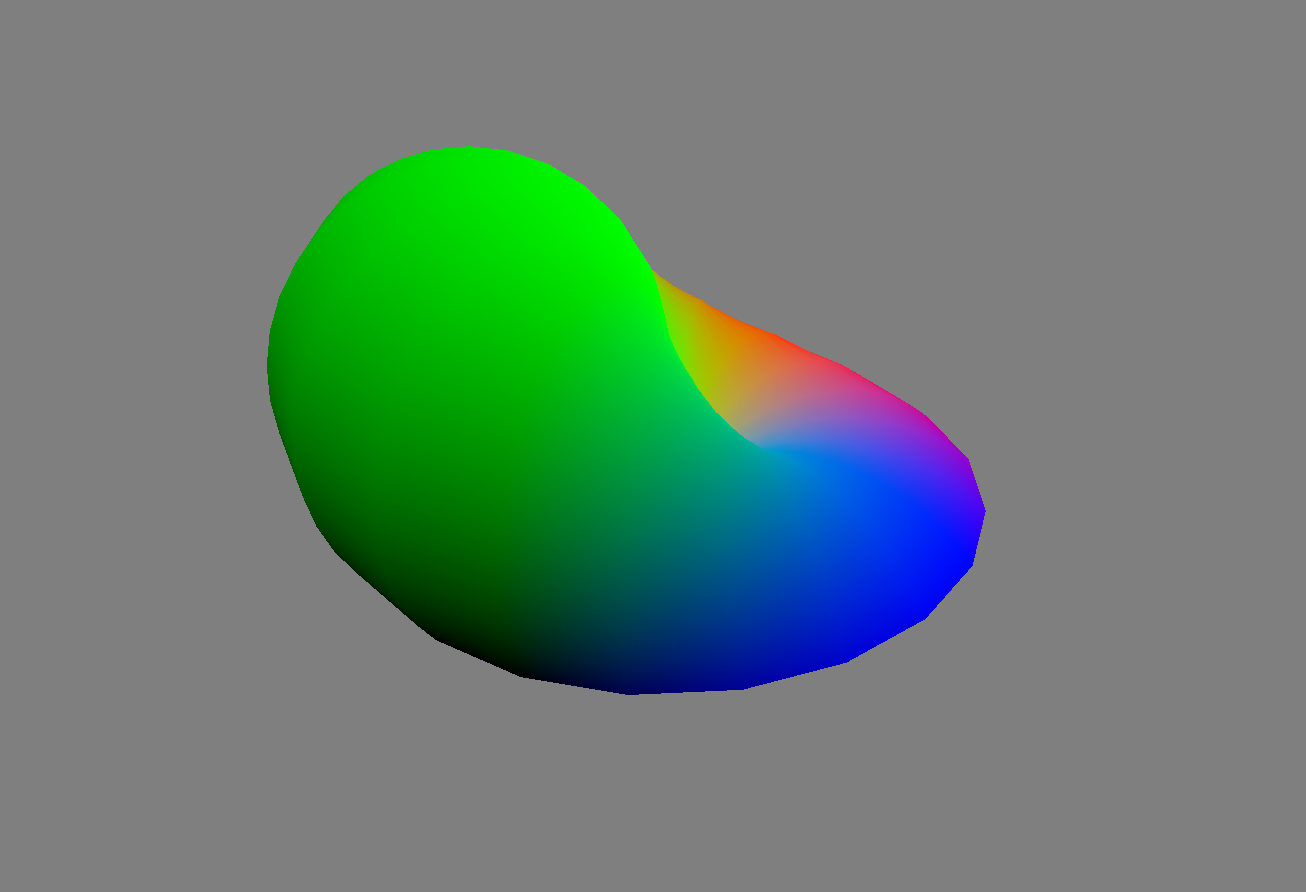
\includegraphics[width=0.33\linewidth]{obrazky-figures/HSH2.png}
    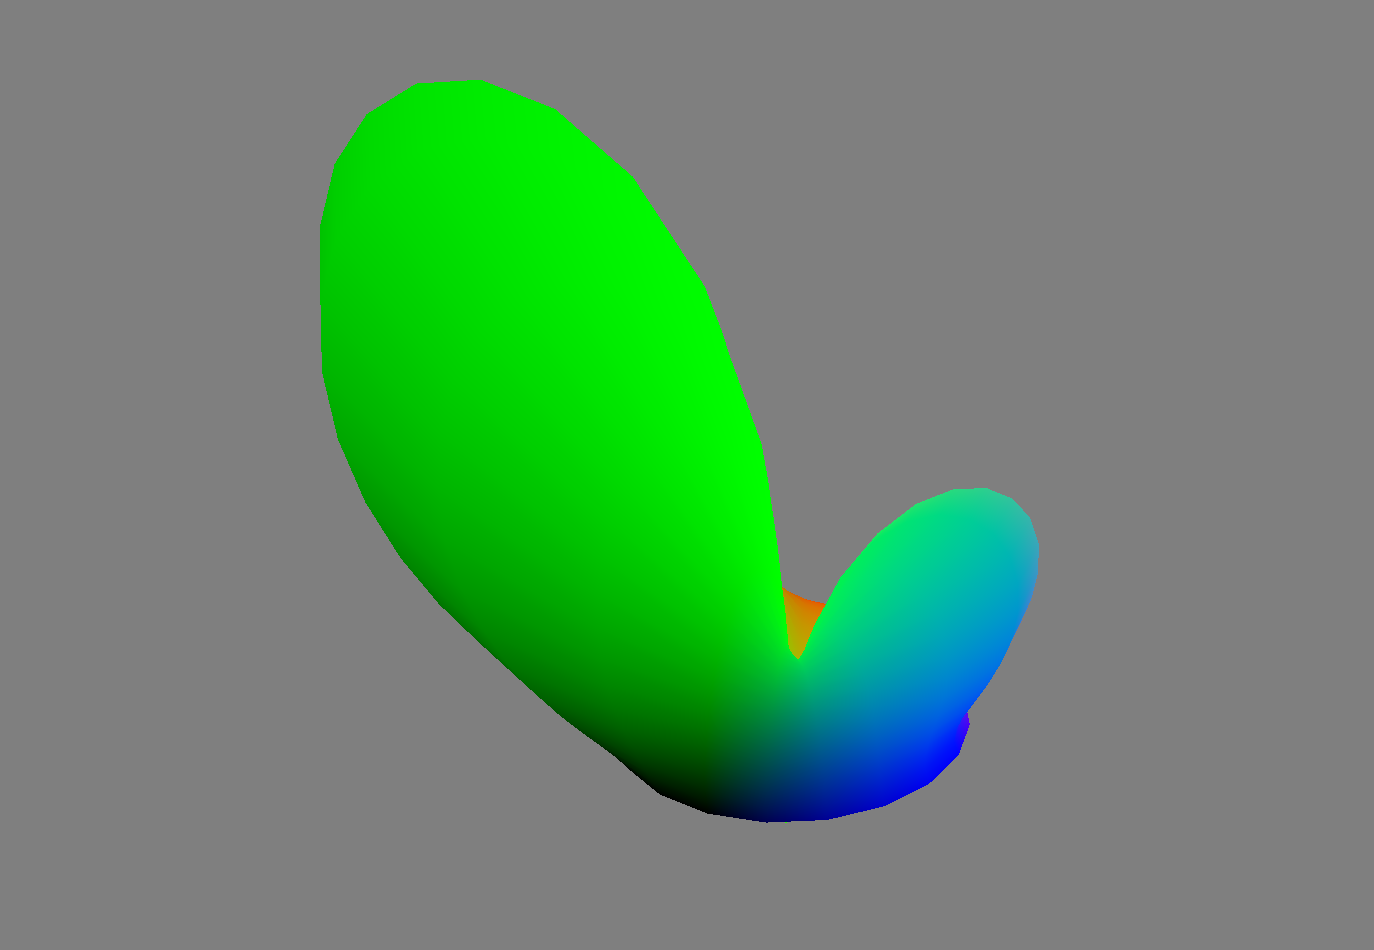
\includegraphics[width=0.325\linewidth]{obrazky-figures/HSH3.png}
    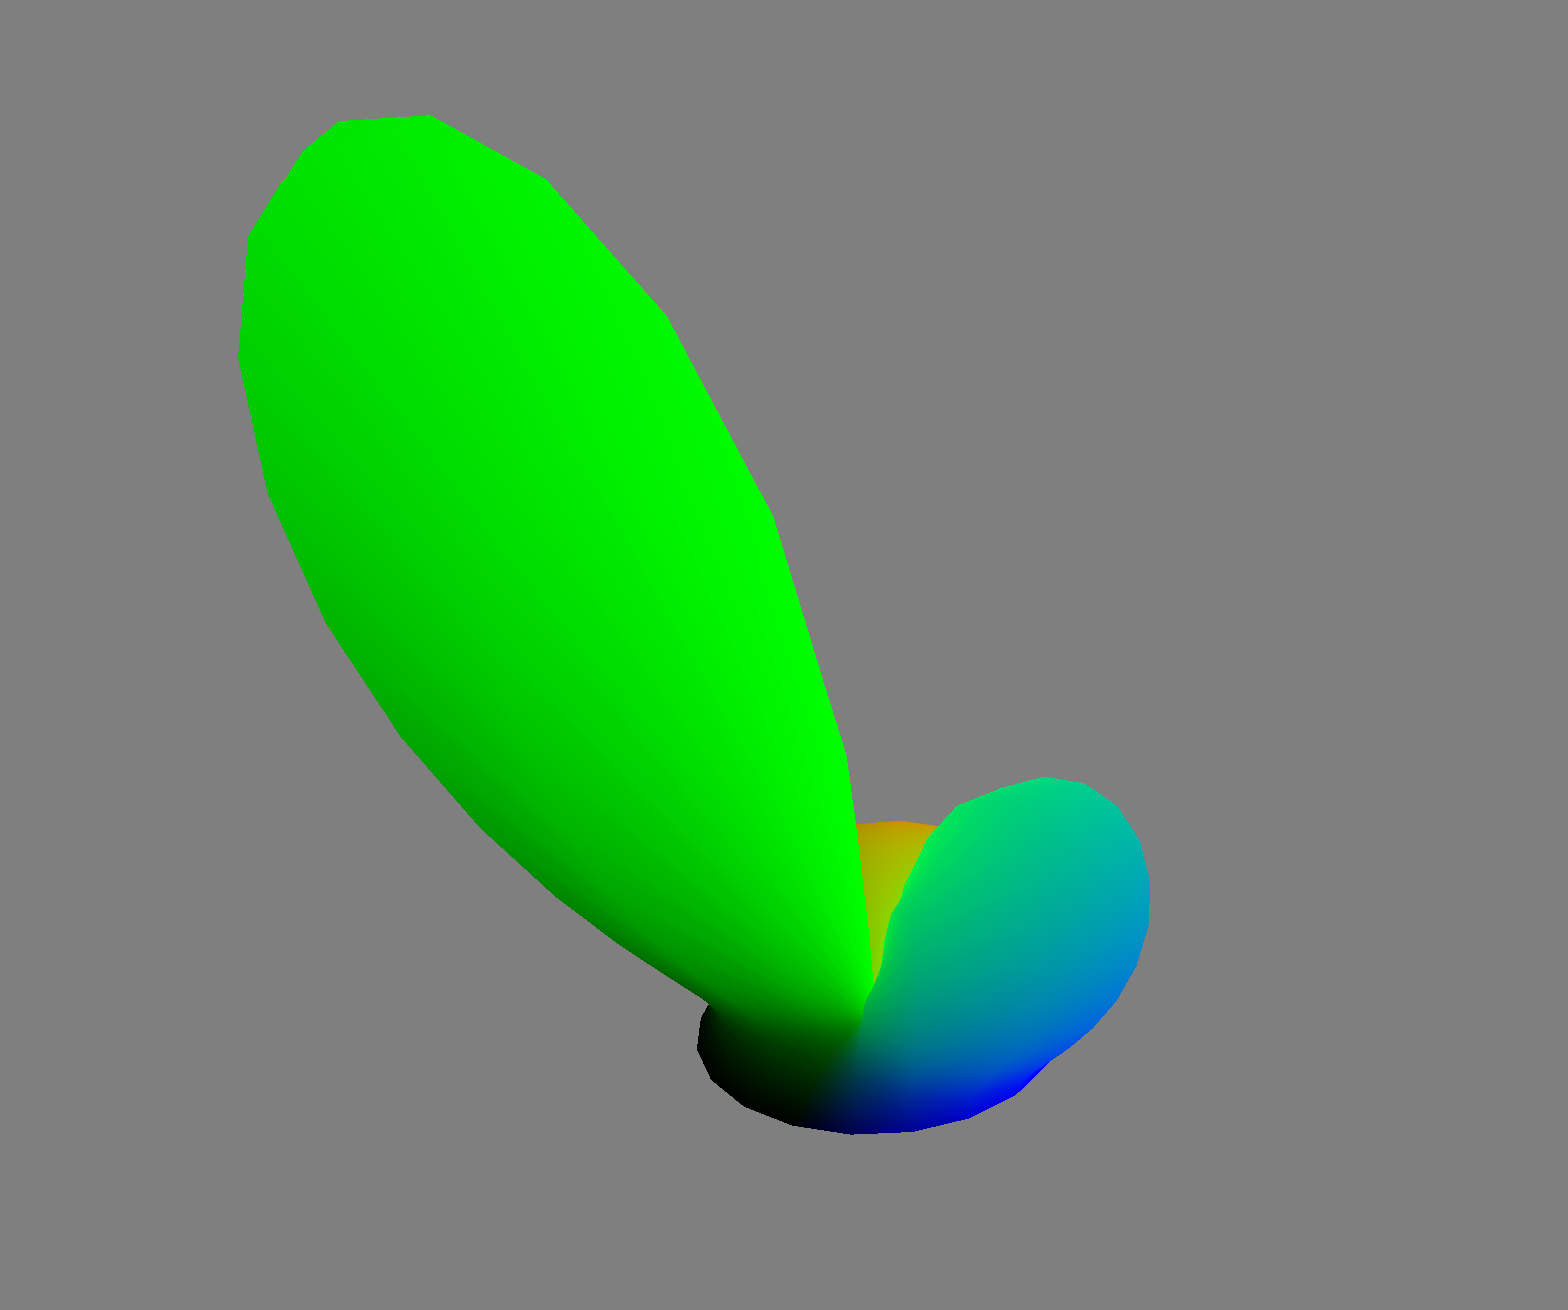
\includegraphics[width=0.358\linewidth]{obrazky-figures/HSH4.png}
    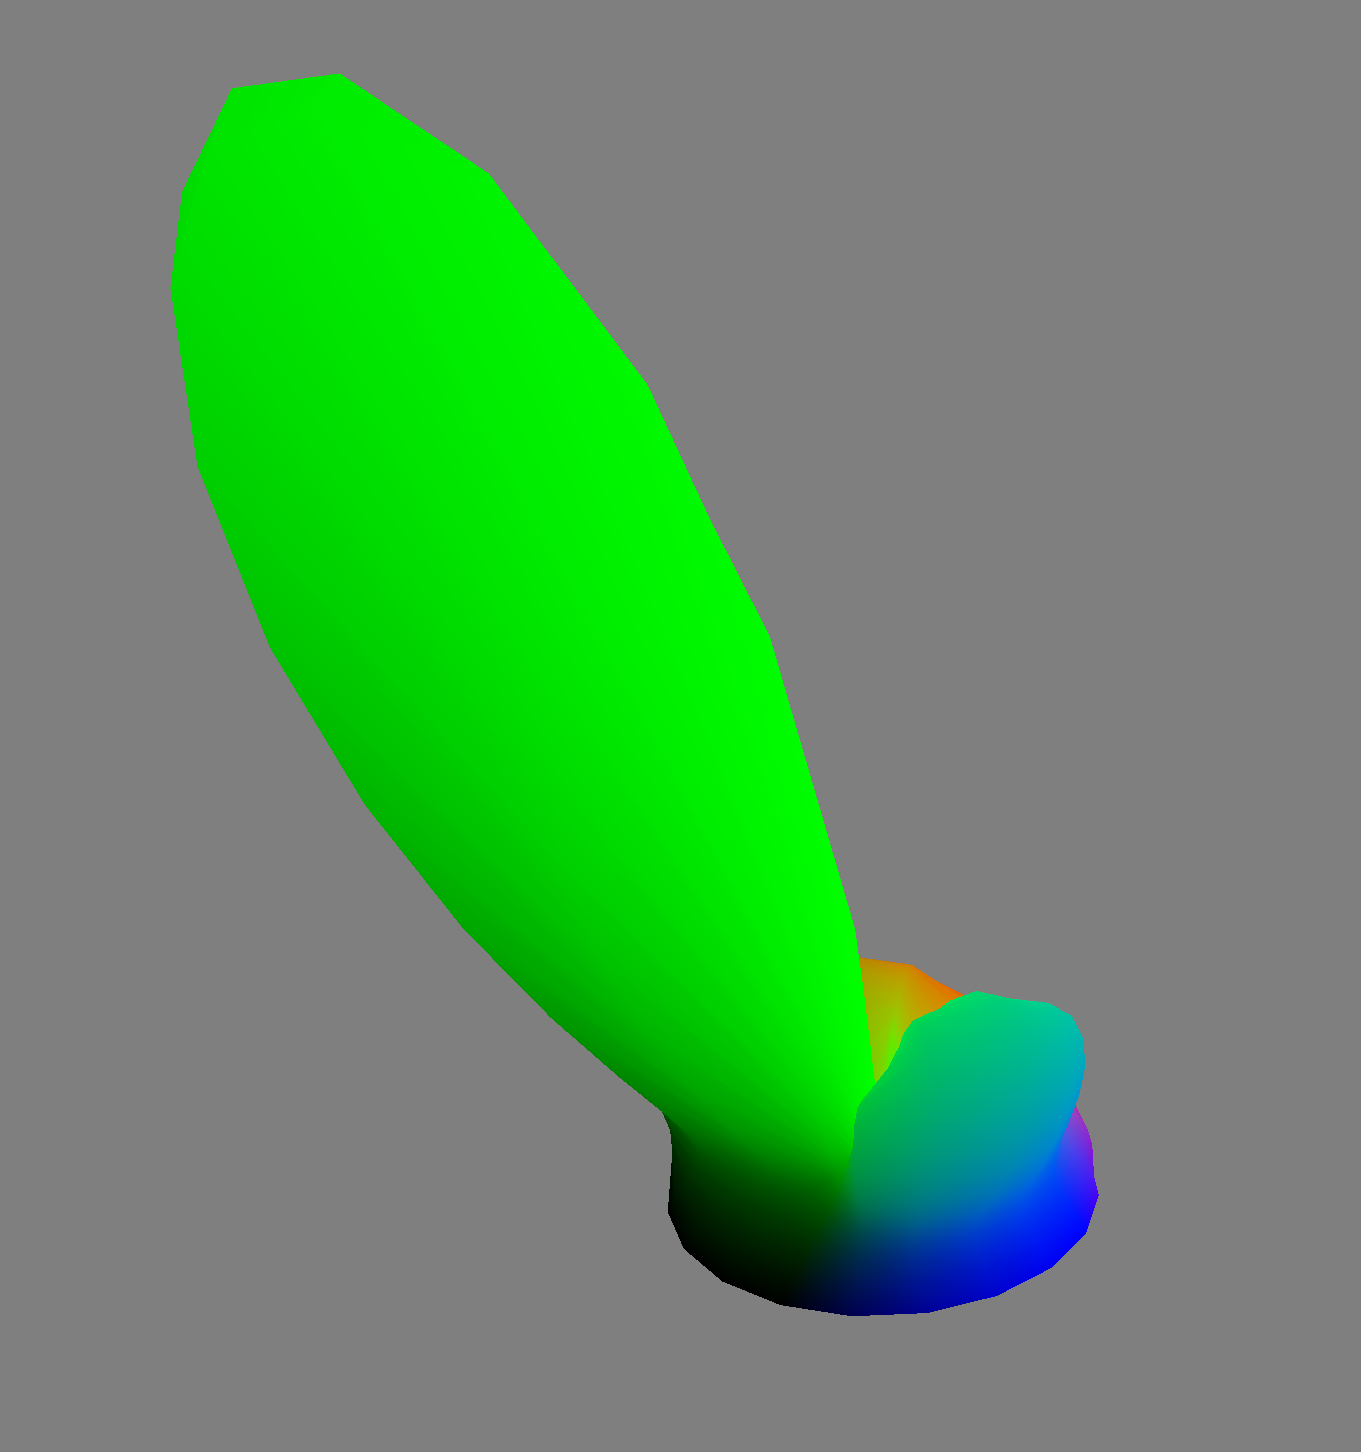
\includegraphics[width=0.282\linewidth]{obrazky-figures/HSH5.png}
    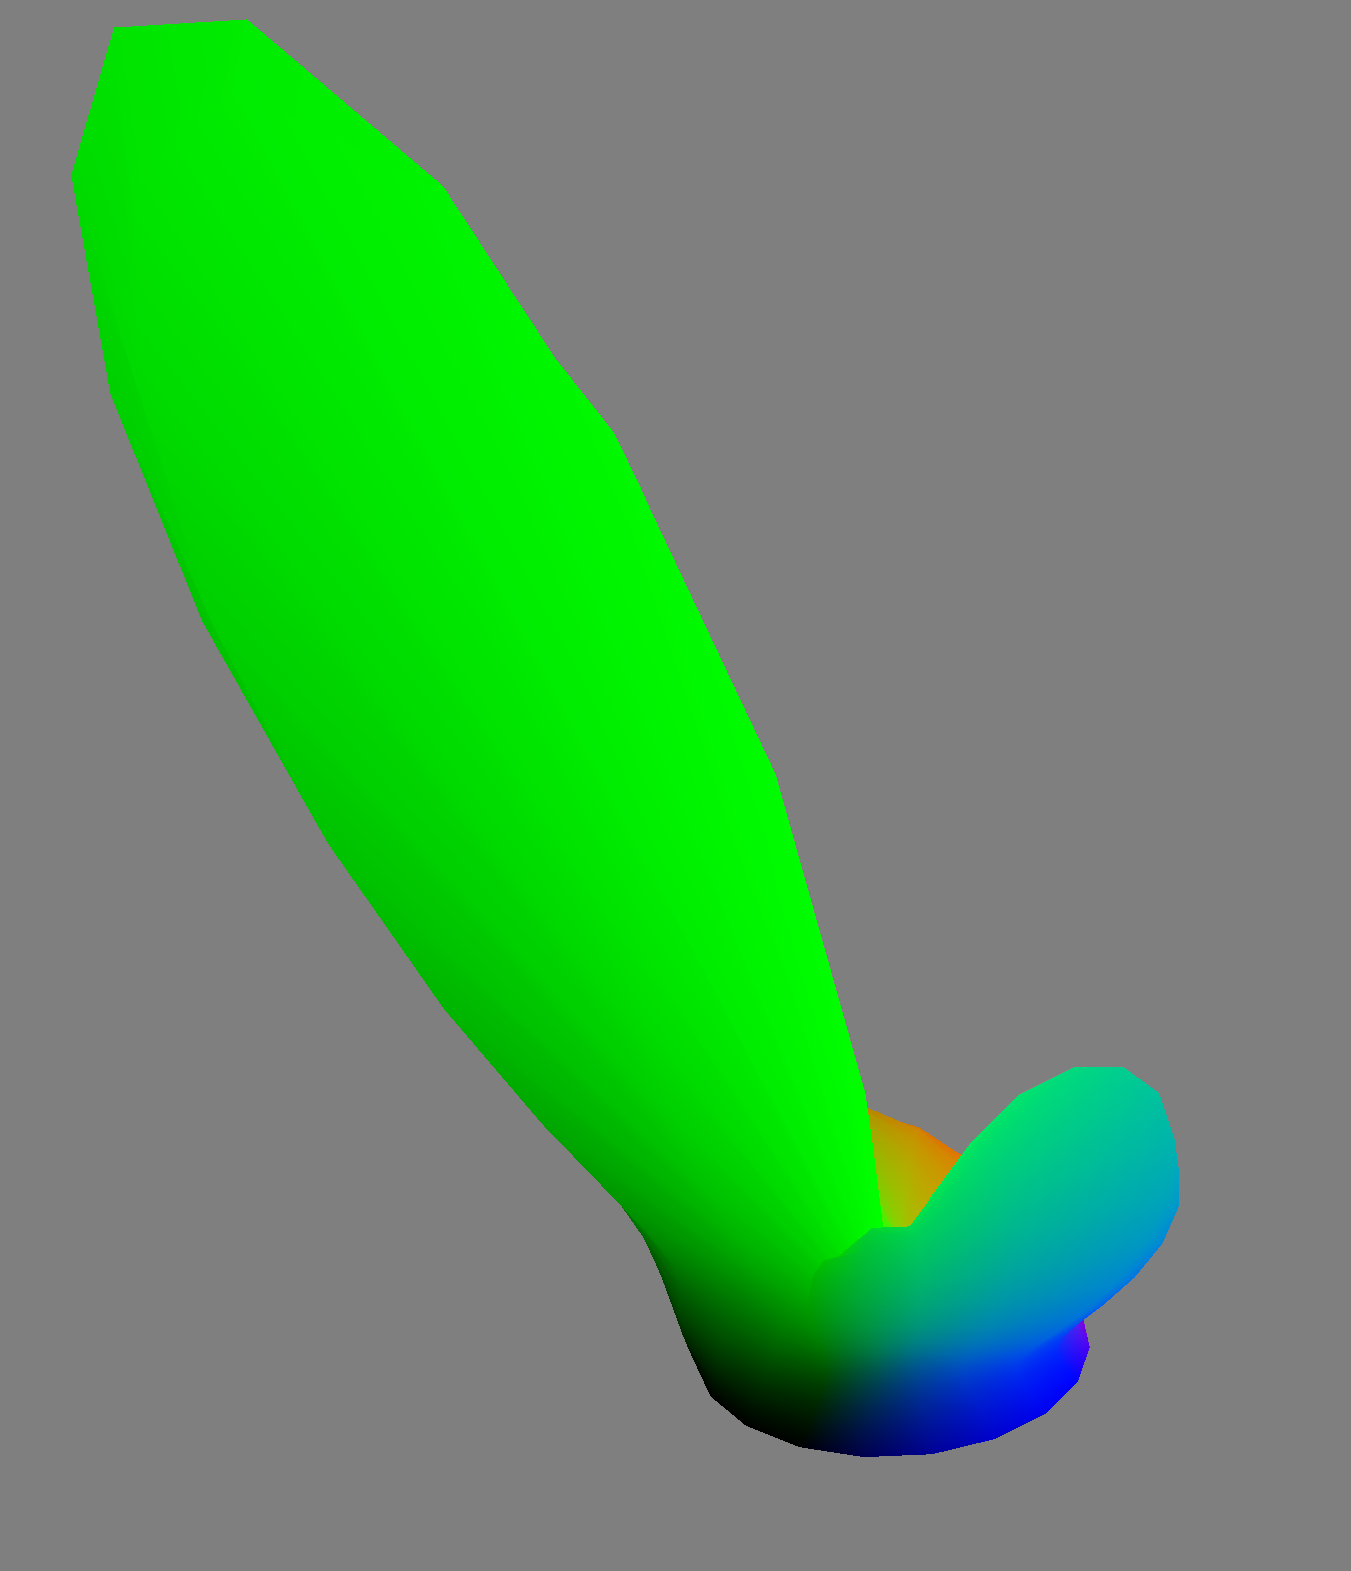
\includegraphics[width=0.258\linewidth]{obrazky-figures/HSH6.png}
    \caption{Úrovne zanorenia HSH funkcií}
\end{figure*}

\begin{figure*}[b!]\label{HSGPorovnanie}
    \centering
    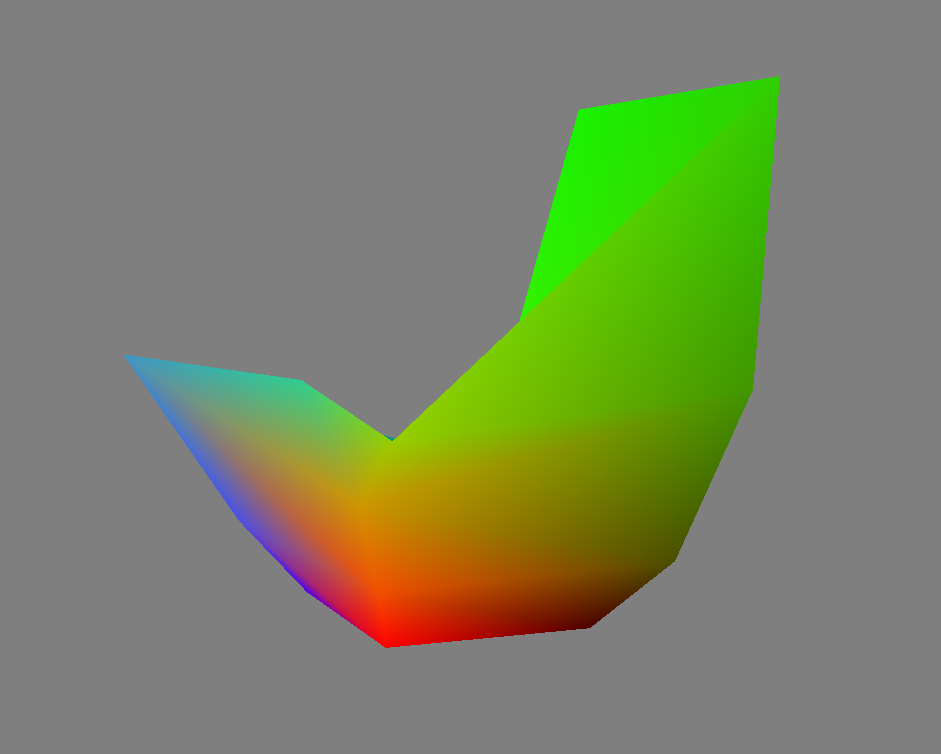
\includegraphics[width=0.45\linewidth]{obrazky-figures/5x5.png}
    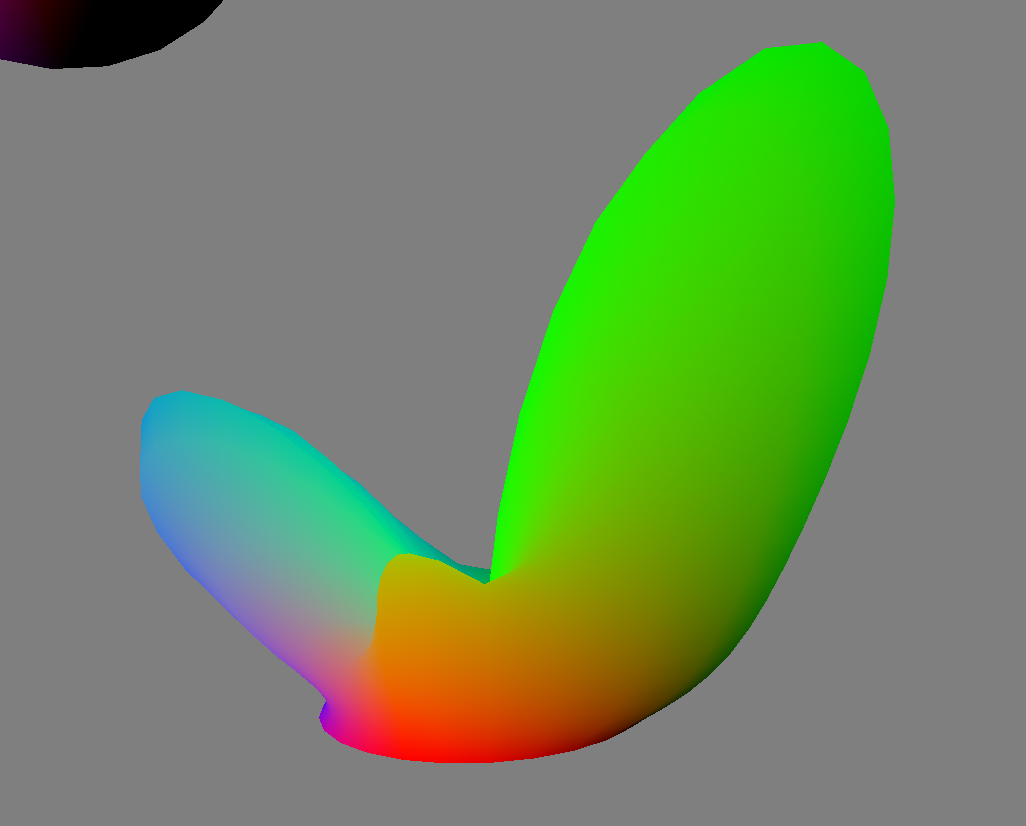
\includegraphics[width=0.45\linewidth]{obrazky-figures/25x25.png}
    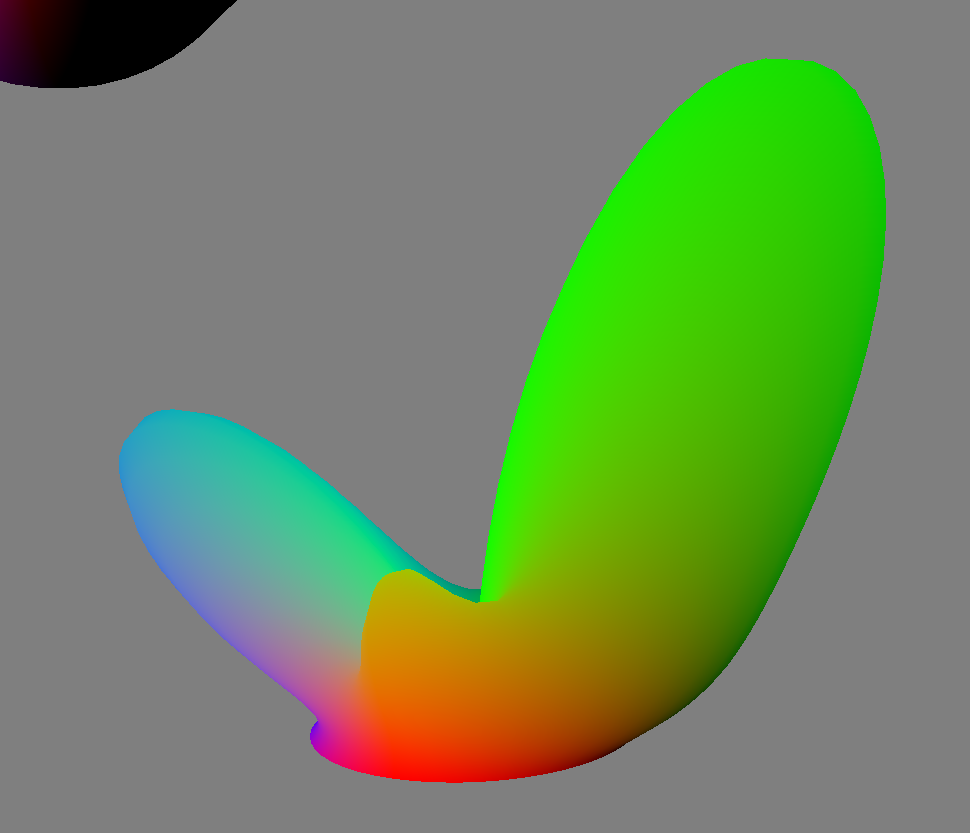
\includegraphics[width=0.45\linewidth]{obrazky-figures/50x50.png}
    \caption{Rozdiely medzi kvalitou hemisférového objektu}
\end{figure*}

\chapter{Záver}
Cieľom práce bolo načítať grafické dáta používané vo vedeckej oblasti ako mračná bodov alebo hemisférické harmonické funkcie a zobraziť ich nad scénami zo vstupných súborov pre Mitsuba renderer. Následne bolo cieľom zobraziť závislosť medzi mračnom bodov a~objektami v~scéne pomocou tepelných máp. Tento cieľ bol splnený.

Teoretické vedomosti ohľadom dátových typov a operácií nad nimi boli naštudované a~opísané v~kapitole \ref{Teoria}. Následný spôsob vizualizácie týchto dát a operácií bol navrhnutý v~sekciách \ref{DataNavrh} a \ref{OperationsNavrh}. Implementácia návrhov bola detailne popísaná v~kapitole \ref{Implementacia}.

Aplikácia dokáže načítať a zobraziť mračno bodov z~vysoko konkrétneho formátu súboru, ktorý nieje verejne používaný, Následne vie načítať scénu zo vstupného formátu pre~Mitsuba renderer a uložiť a zobraziť objekty formátu Wavefront .obj. Aplikácia vie zobraziť hemisférické harmonické funkcie nad bodmi z~mračna. Takisto vie zobraziť tepelné mapy nad objektami podľa počtu bodov v~blízkosti objektu. Tieto operácie sú ovládané a~upravovateľné používateľom vďaka užívateľskému rozhraniu.

Počas práce som sa naučil spôsoby ukladania a renderovania objektov na grafickej karte. Následne som sa naučil o~mračnách bodov a o~shadovacích technikách pri farbení tepelných máp. Veľa som sa naučil aj o~hemisférických harmonických funkciách a o~ich použití v~grafickom odbore.

Rozšírenia práce by mohli zahrňovať viaceré funkcie, napríklad analýzu paprskov svetla v~scéne. Takisto by sa mohlo optimalizovať vykresľovanie tepelných máp. Upraviť by sa~moh\-lo aj filtrovanie bodov pre jednotlivé objekty, ktoré by mohlo lepšie určovať body v~blízkosti vrcholov objektu a tým znížiť zaťaženie grafických kariet pri renderovaní tepelných máp. Ďalším vylepšením by mohlo byť pridanie možností nastavenia operácií v~užívateľskom rozhraní, alebo optimalizácia načítania bodov v~mračne pri mračnách s~väčším objemom dát.

%===============================================================================

% Pro kompilaci po částech (viz projekt.tex) nutno odkomentovat
%\end{document}

  \fi
  
  % Kompilace po částech (viz výše, nutno odkomentovat a zakomentovat input výše)
  % Compilation piecewise (see above, it is necessary to uncomment it and comment out input above)
  %\subfile{chapters/projekt-01-uvod-introduction}
  % ...
  %\subfile{chapters/projekt-05-zaver-conclusion}

  % Pouzita literatura / Bibliography
  % ----------------------------------------------
\ifslovak
  \makeatletter
  \def\@openbib@code{\addcontentsline{toc}{chapter}{Literatúra}}
  \makeatother
  \bibliographystyle{bib-styles/Pysny/skplain}
\else
  \ifczech
    \makeatletter
    \def\@openbib@code{\addcontentsline{toc}{chapter}{Literatura}}
    \makeatother
    \bibliographystyle{bib-styles/Pysny/czplain}
  \else 
    \makeatletter
    \def\@openbib@code{\addcontentsline{toc}{chapter}{Bibliography}}
    \makeatother
    \bibliographystyle{bib-styles/Pysny/enplain}
  %  \bibliographystyle{alpha}
  \fi
\fi
  \begin{flushleft}
  \bibliography{projekt-20-literatura-bibliography}
  \end{flushleft}

  % vynechani stranky v oboustrannem rezimu
  % Skip the page in the two-sided mode
  \iftwoside
    \cleardoublepage
  \fi

  % Prilohy / Appendices
  % ---------------------------------------------
  \appendix
\ifczech
  \renewcommand{\appendixpagename}{Přílohy}
  \renewcommand{\appendixtocname}{Přílohy}
  \renewcommand{\appendixname}{Příloha}
\fi
\ifslovak
  \renewcommand{\appendixpagename}{Prílohy}
  \renewcommand{\appendixtocname}{Prílohy}
  \renewcommand{\appendixname}{Príloha}
\fi
%  \appendixpage

% vynechani stranky v oboustrannem rezimu
% Skip the page in the two-sided mode
%\iftwoside
%  \cleardoublepage
%\fi
  
\ifslovak
%  \section*{Zoznam príloh}
%  \addcontentsline{toc}{section}{Zoznam príloh}
\else
  \ifczech
%    \section*{Seznam příloh}
%    \addcontentsline{toc}{section}{Seznam příloh}
  \else
%    \section*{List of Appendices}
%    \addcontentsline{toc}{section}{List of Appendices}
  \fi
\fi
  \startcontents[chapters]
  \setlength{\parskip}{0pt} 
  % seznam příloh / list of appendices
  % \printcontents[chapters]{l}{0}{\setcounter{tocdepth}{2}}
  
  \ifODSAZ
    \setlength{\parskip}{0.5\bigskipamount}
  \else
    \setlength{\parskip}{0pt}
  \fi
  
  % vynechani stranky v oboustrannem rezimu
  \iftwoside
    \cleardoublepage
  \fi
  
  % Přílohy / Appendices
  \ifenglish
    \input{projekt-30-prilohy-appendices-en}
  \else
    % Tento soubor nahraďte vlastním souborem s přílohami (nadpisy níže jsou pouze pro příklad)

% Pro kompilaci po částech (viz projekt.tex), nutno odkomentovat a upravit
%\documentclass[../projekt.tex]{subfiles}
%\begin{document}

% Umístění obsahu paměťového média do příloh je vhodné konzultovat s vedoucím
%\chapter{Obsah přiloženého paměťového média}

\chapter{Obsah priloženého média}
Príloha obsahuje dátovú štruktúru priloženého média a informácie o jeho súboroch a priečinkoch.
\begin{itemize}
    \item \verb|xduric05.pdf| -- PDF verzia bakalárskej prace
    \item \verb|xduric05/| -- Zdrojové kódy pre textovú časť bakalárskej práce
    \item \verb|obj/| -- .obj súbory pre predom určené tvary objektov
    \item \verb|shaders/| -- Shadery pre aplikáciu
    \item \verb|scenes/| -- Demo scény pre program
    \item \verb|camera.py| -- Kamerový modul
    \item \verb|FileDialog.py| -- Modul na vizuálny výber vstupných súborov
    \item \verb|objLoader.py| -- Modul na čítanie .obj súborov
    \item \verb|read_point_cloud.py| -- Modul na parsovanie súborov s mračnom bodov
    \item \verb|read_xml_scene.py| -- Modul na parsovanie XML súborov
    \item \verb|main.py| -- Hlavný kód aplikácie
    \item \verb|README.txt| -- Informácie o aplikácii, inštalácii a spustení
    \item \verb|requirements.txt| -- Prerekvizity programu použité pri inštalácii
    \item \verb|video.mp4| -- Demonštračné video
\end{itemize}

%\chapter{Konfigurační soubor}

%\chapter{RelaxNG Schéma konfiguračního souboru}

%\chapter{Plakát}



% Pro kompilaci po částech (viz projekt.tex) nutno odkomentovat
%\end{document}

  \fi
  
  % Kompilace po částech (viz výše, nutno odkomentovat)
  % Compilation piecewise (see above, it is necessary to uncomment it)
  %\subfile{projekt-30-prilohy-appendices}
  
\end{document}
